%!TeX spellcheck=en_US
\documentclass[11pt,
               a4paper,
               bibtotoc,
               idxtotoc,
               headsepline,
               footsepline,
               footexclude,
               BCOR12mm,
               DIV13,
               openany,   % using this removes blank pages around part / chapter starts.
%               oneside    % include this if you have to print only one page per sheet of paper.
               ]
               {scrbook}

%%% SETTINGS

% no word wrapping
%\righthyphenmin=62
%\lefthyphenmin=62
% fewer hyphens
\usepackage{microtype}

% german symbols
\usepackage[utf8]{inputenc}

% strikethrough by \sout
\usepackage[normalem]{ulem}

% insert graphics
\usepackage{graphicx}
% more flexible figures e.g. graphics with captions beside them
\usepackage{floatrow}
% more flexible captions.
% Use \captionsetup{options} to configure,
% use it in an environment for local setup
\usepackage{caption}
% subfigures (see template):
\usepackage{subcaption}

% more control of enumerations and itemizations
\usepackage{enumitem}
% less space between items
\setlist[itemize]{itemsep=0cm}
\setlist[enumerate]{itemsep=0cm}
% more customizeable tables (e.g. multiple lines per cell)
\usepackage{tabularx}
% fix for vertical centering
\usepackage{ragged2e}
\renewcommand\tabularxcolumn[1]{>{\Centering}m{#1}}
% column types with multiple lines and formatting
\usepackage{array}
\newcolumntype{C}{>{\centering\arraybackslash}X}
\newcolumntype{R}{>{\raggedleft\arraybackslash}X}
\newcolumntype{L}{>{\raggedright\arraybackslash}X}
% merge multiple rows \multirow{2}{*}{bla} & \\ &
\usepackage{multirow}
% activate for tables with page breaking
%\usepackage{ltablex}
% fix for table movement and itemizations
%\keepXColumns

% fix for dynamics spaces after custom commands
\usepackage{xspace}

% tabbing: use with \tab
\usepackage{tabto}
\TabPositions{4cm}

%% fancy math
% propper matrices, underbrace text
%\usepackage{amsmath}
\usepackage{mathtools}
% special symbols e.g. squares
\usepackage{amssymb}

%% plotting
\usepackage{pgfplots}
\usepgfplotslibrary{fillbetween}

%%Settings for code
% code placement right there
\usepackage{float}
% code coloring
\usepackage{xcolor}
% code listing
\usepackage{listings}

% flexible multi column style
\usepackage{multicol}

% graphs
\usepackage{tikz}
\usetikzlibrary{shapes.geometric, arrows}
% define some elements
\tikzstyle{startstop} = [rectangle, rounded corners, minimum width=3cm, minimum height=1cm,text centered, draw=black, fill=blue!30]
\tikzstyle{arrow} = [thick,->,>=stealth]

% Some code highlighting styles you can use with lstlistings
% C++ code style similar to default eclipse
\lstdefinestyle{eclipse-cpp} {
    captionpos=b,
    language=C++,
    otherkeywords={final},
    basicstyle=\footnotesize,
    numbers=left,
    numberstyle=\small,
    showstringspaces=false,
    tabsize=2,
    frame=single,
    breaklines=true,
    keywordstyle=\bfseries\color[RGB]{127,0,85},
    identifierstyle=\color[RGB]{0,0,192},
    stringstyle=\color[RGB]{42,0,255},
    commentstyle=\color[RGB]{63,127,95},
}

% If no highlighting is intended
\lstdefinestyle{plain}{
}

% fancy algorithms (see template)
\usepackage[ruled, vlined, linesnumbered]{algorithm2e}
\DontPrintSemicolon
\SetKw{KwBy}{by}
\SetKw{KwAnd}{and}

% clickable links and clickable table of content <3
% Options: links with linebreaks
\PassOptionsToPackage{hyphens}{url}\usepackage[bookmarks=false]{hyperref}
\hypersetup{
    colorlinks,
    citecolor=black,
    filecolor=black,
    linkcolor=black,
    urlcolor=black
}
% Alterations to labels used by \autoref{}: Capitalize everyything
\def\chapterautorefname{Chapter}
\def\sectionautorefname{Section}
\def\subsectionautorefname{Subsection}
\def\algorithmautorefname{Algorithm}
\def\subfigureautorefname{Figure}
% for fully custon stuff use:
% \hyperref[custom:foo]{Custom~\ref*{custom:foo}}


\usepackage{lipsum} % for filling pages with stuff
\usepackage{algpseudocode}

% -------------------------------------------------------------------------------
% --------------------------------- Thesis Info ---------------------------------
% -------------------------------------------------------------------------------

% set title, authors and stuff for the cover
% docytype needs xspace because it is used within text.
\def\doctype{Bachelor's Thesis\xspace}
%\def\doctype{Master's Thesis\xspace}
%\def\doctype{Guided Research\xspace}
%\def\doctype{Interdisciplinary Project\xspace}
\def\studyProgram{Informatics}
\def\title{Efficient Bayesian Inference of Hydrological Model Parameters: Implementation of a Parallel Markov Chain Monte Carlo Approach}
% don't try translate every technical term if it would sound off
\def\titleGer{Effiziente Bayesschen Inferenz der Parameter von der hydrologischen Modelle: Implementierung eines Markov-Chain-Monte-Carlo-Verfahrens im parallelen Modus}
\def\author{Chengjie Zhou}
% Prof
\def\supervisor{Univ.-Prof. Dr. Hans-Joachim Bungartz}
% PhD Candidate
\def\advisor{Ivana Jovanovic Buha, M.Sc. (hons)}
\def\date{09.08.2024}

\begin{document}
\frontmatter
% -------------------------------------------------------------------------------
% ---------------------------------- COVERPAGE ----------------------------------
% -------------------------------------------------------------------------------

% correct BCOR - undo at the end !!!
\def\bcorcor{0.15cm}
\addtolength{\hoffset}{\bcorcor}
\thispagestyle{empty}
\vspace{4cm}
\begin{center}
    
\includegraphics[width=4cm]{templateStuff/tumlogo.pdf}\\[5mm]
    \huge SCHOOL OF COMPUTATION, INFORMATION AND TECHNOLOGY\\[5mm]
    \large DER TECHNISCHEN UNIVERSITÄT MÜNCHEN\\[24mm]

    {\Large \doctype in \studyProgram}\\[20mm]
    {\huge\bf \title\par}
    \vspace{15mm}
    {\LARGE  \author}
\end{center}

\cleardoubleemptypage

% -------------------------------------------------------------------------------
% ---------------------------------- TITLEPAGE ----------------------------------
% -------------------------------------------------------------------------------

\def\bcorcor{0.15cm}
\addtolength{\hoffset}{\bcorcor}
\thispagestyle{empty}
\vspace{10mm}
\begin{center}
    
\includegraphics[width=4cm]{templateStuff/tumlogo.pdf}\\[5mm]
	\huge SCHOOL OF COMPUTATION, INFORMATION AND TECHNOLOGY\\[5mm]
	\large DER TECHNISCHEN UNIVERSITÄT MÜNCHEN\\[24mm]
	{\Large \doctype in \studyProgram}\\[20mm]
	{\LARGE\bf \title}\\[10mm]
	{\LARGE\bf \titleGer}\\[10mm]
	\begin{tabular}{ll}
		\Large Author:      	& \Large \author \\[2mm]
		\Large Supervisor:  	& \Large \supervisor\\[2mm]
		\Large Advisor:			& \Large \advisor\\[2mm]
		\Large Date:       		& \Large \date
	\end{tabular}
\end{center}

% undo BCOR correction
\addtolength{\hoffset}{\bcorcor}
\newpage

% -------------------------------------------------------------------------------
% ---------------------------------- DISCLAIMER ---------------------------------
% -------------------------------------------------------------------------------

\cleardoubleemptypage

\thispagestyle{empty}
\vspace*{0.7\textheight}
\noindent
I confirm that this \MakeLowercase{\doctype} is my own work and I have documented all sources and material used.\\

\vspace{15mm}
\noindent
Munich, \date \hspace{5cm} \author
\cleardoubleemptypage

% -------------------------------------------------------------------------------
% ------------------------------- ACKNOWLEDGEMENTS ------------------------------
% -------------------------------------------------------------------------------

\phantomsection
\addcontentsline{toc}{chapter}{Acknowledgements}
\vspace*{2cm}
\begin{center}
    {\Large \bf Acknowledgements}
\end{center}
\vspace{1cm}

\lipsum[1]

\cleardoublepage

% -------------------------------------------------------------------------------
% ---------------------------------- ABSTRACT -----------------------------------
% -------------------------------------------------------------------------------

\phantomsection
\addcontentsline{toc}{chapter}{Abstract}
\vspace*{2cm}
\begin{center}
    {\Large \bf Abstract}
\end{center}
\vspace{1cm}
Bayesian inference of hydrological model parameters is crucial for improving the accuracy and reliability of hydrological model executions. This thesis presents the implementation of the Markov Chain Monte Carlo (MCMC) approach to enhance the accuracy and the efficiency of Bayesian parameter estimation, with a predominant focus on the parallel version of the algorithms. Results regarding the accuracy and efficiency of the Bayesian inference are analyzed through comparison metrics and displayed using detailed visualizations so that the relationship between algorithm implementation variants and the results can be comprehended. Besides, the relationship between the training time series for the Markov chain Monte Carlo algorithms is also considered. By investigating these aspects of the algorithms and the data set, more insights regarding the performance and the result of Bayesian inference can be gained, enabling more practical and scalable applications in hydrological modeling.
\cleardoublepage

\phantomsection
\addcontentsline{toc}{chapter}{Zusammenfassung}
\vspace*{2cm}
\begin{center}
    {\Large \bf Zusammenfassung}
\end{center}
\vspace{1cm}
Das Verfahren der Bayesschen Inferenz für die Parameter der hydrologischen Modelle spielt eine bedeutende Rolle bei der Ausführung der hydrologischen Modelle, vor allem bezüglich der Genauigkeit und der Zuverlässigkeit. Dieses Thema wird in dieser Arbeit auseinandergesetzt, indem man das Verfahren die Algorithmen zum Markov-Chain-Monte-Carlo-Verfahren implementiert, vor allem mit der Eigenschaft von dem Parallelrechner, damit sich die Genauigkeit und die Effizienz von der Bayesschen Schätzung der Parameter verbessern. Die Ergebnisse bezüglich der Genauigkeit und der Effizienz der Bayesschen Inferenz werden mithilfe der Vergleichsmetriken analysiert, wodurch sie ausführlich visualisiert werden, sodass die Beziehungen zwischen den verschiedenen Implementierungsvarianten und den Ergebnissen klar dargestellt werden können. Außerdem wird die Beziehung zwischen der Wahl der Trainingsdatensätze in Form einer Zeitreihe und die Ergebnisse einer Bayesschen Inferenz beobachtet. Durch die Analyse dieser Aspekte von den spezifischen Implementierungen der Algorithmen und den Datensätzen erwirbt man Kenntnisse über die Leistung und die Ergebnisse der Bayesschen Inferenz, sodass praktische und skalierbare Anwendung bei der hydrologischen Modellierung angewendet werden können.
\cleardoublepage

% -------------------------------------------------------------------------------
% ------------------------------ TABLE OF CONTENTS ------------------------------
% -------------------------------------------------------------------------------

\tableofcontents
\thispagestyle{empty}
\cleardoubleemptypage

% -------------------------------------------------------------------------------
% --------------------------------- MAIN MATTER ---------------------------------
% -------------------------------------------------------------------------------

\mainmatter
\part{Introduction and Background}
\chapter{Introduction}
\chapter{Introduction to Markov Chain Monte Carlo and Bayesian Inference}

In this chapter, the basic theory of Markov chain Monte Carlo algorithms will be introduced, with an example provided alongside visualizations. Afterwards, the idea of Bayesian inference will be explained, including the instantiation of this problem using the Markov chain Monte Carlo algorithm.

\section{The Idea of Markov Chain Monte Carlo}
Markov chain Monte Carlo (abbr. MCMC) is an algorithm that performs sampling. General usage of the Markov chain Monte Carlo algorithm started in the fields of chemistry, biochemistry, and physics up until after 1990 when it was also adopted by the field of statistics and scientific computing~\cite{mcmc_handbook}. The general idea of the Markov chain Monte Carlo includes, as its name suggests, a combination of the Monte Carlo methods and the usage of Markov chains. The Monte Carlo methods solve numerical problems by repeatedly generating random numbers~\cite{monte_carlo_methods}, whereas the Markov chains provide this algorithm a property so that each sample that is generated depends on the sample that is generated before~\cite{mcmc_wang}.

The Markov chain Monte Carlo tries to sample an unknown target distribution using a proposal distribution that completely lies above the target distribution. The selection proposal distribution is crucial to the success of the algorithm, since it may lead to different behaviors of convergence and acceptance probability~\cite{mcmc_handbook}. The core of the Markov chain Monte Carlo is the application of a Markov chain, where the Monte Carlo integration is used. Given a distribution $\pi(\cdot)$ and its probability function $f(\cdot)$, a typical Monte Carlo simulation would perform the following mathematical approximation:
\begin{align}
\mathbb{E}[f(X)] \approx \frac{1}{n}\sum_{i=1}^{n}f(X_i)
\end{align}
where $\{X_i | i\in[1, n]\}$ is the sample space that is drawn from the distribution $\pi(\cdot)$~\cite{mcmc_practice}. Since this approximation is used on a Markov chain, each sample from the sample space is dependent on the sample before. In Markov chain Monte Carlo, this dependence is given by a transition kernel that is essentially a conditional distribution $\Pr[X_{i+1}|X_i]$~\cite{mcmc_practice}. In other words: After the last sample was generated, a distribution that takes this generated sample as a parameter is created. The next sample is then generated based on this newly created sample, which creates a dependence between both samples. Markov chains Monte Carlo functions thanks to a property called ergodicity that is shared by all Markov chains. The ergodic theorem states that the distribution of the states on the chain converges to a certain stationary distribution regardless of the starting state, as time approaches infinity~\cite{ergodicity}. This property could be applied in the case of Markov chain Monte Carlo as well. The starting states that do not sample from the stationary distribution before the ergodic states can be regarded as "burn-in states" and should be discarded. Thus, the approximation of the Monte Carlo simulation can be altered to
\begin{align}
\mathbb{E}[f(X)] \approx \frac{1}{n-b}\sum_{i=b + 1}^{n}f(X_i)
\end{align}
where $b$ denotes the position of the last state in the burn-in phase that should be discarded~\cite{mcmc_practice}. The determination of the burn in phase plays an important part in terms of the sample space accuracy and will be discussed later in this thesis in a more detailed manner.

A crucial prerequisite of the Markov chain Monte Carlo algorithm is the detailed balance condition. The ergodicity property after the burn-in period for every Markov chain can be mathematically defined as:
\begin{align}
\forall X, Y\in S. \ \pi(X) \Pr[Y|X] = \pi(Y) \Pr[X|Y]
\end{align}
\cite{mcmc_practice} where $S$ is the set of the state of a Markov chain. From this equation, we can derive the following property:
\begin{align}
\int \pi(X) \Pr[Y|X] dX= \int \pi(Y) \Pr[X|Y] dX =\pi(X_j)
\end{align}
What this equation essentially points out is that if $X$ is sampled from the stationary distribution $\pi(\cdot)$, $Y$ will also be from this stationary distribution~\cite{mcmc_practice}. This corresponds to the idea of ergodicity and proves that using the detailed balance equation, all of the subsequent samples will eventually connect stationary and target distribution from the very beginning.

\section{The Metropolis-Hastings Algorithm}
Metropolis-Hastings is a widely used algorithm that performs Markov chain Monte Carlo sampling. It is extremely versatile and often used to sample multivariate distribution. It was extensively used in the physics field, but later on also in the statistics field~\cite{understanding_mh}.

As mentioned before, the Markov chain Monte Carlo algorithms use a transition kernel to create dependence between two states.

The main idea is that for each iteration, a sample is drawn from the target distribution. For the generation of the next state, a distribution that takes the last sampled data point as a parameter will be created so that the new sample can be drawn from the newly created distribution~\cite{mcmc_practice}. An acceptance probability is then calculated using the following formula:

\begin{align}
\alpha(X, Y) = \min (\frac{\pi(Y)q[Y|X]}{\pi(X)q[X|Y]}, 1)
\end{align}
where $q[X|Y]$ denotes the proposal density from $X$ to $Y$. With the proposal density multiplied by the acceptance probability, the transition probability is derived:

\begin{align}
\Pr[X|Y] = q(X|Y) A(Y, X)
\end{align}
Due to the detailed balance equation~\cite{mcmc_practice}:
\begin{align}
\pi(X) q(Y|X) A(X, Y) = \pi(Y) q(X|Y) A(Y, X)
\end{align}
Bringing the ratio of the acceptance probability to the left
\begin{align}
\frac{A(Y, X)}{A(X, Y)} = \frac{\pi(Y)q[Y|X]}{\pi(X)q[X|Y]} := \alpha(X, Y)
\end{align} 
As we can see, the acceptance probability of the Metropolis-Hastings algorithm is calculated based on the ratio of the acceptance density from the old to the newly generated sample point to the acceptance density from the newly to the old generated sample point. However, since the probability space adds up to one, the maximum acceptance probability can not exceed one. Therefore, a minimum condition must be added.

A special case of the Metropolis-Hastings algorithm is the Metropolis algorithm. The Metropolis algorithm applies a symmetric distribution as the transition kernel, such as a normal distribution~\cite{metropolis}. Due to the symmetry, the proposal density $q[Y|X]$ equals to $q[X|Y]$. The idea is that the position of the density of the newly generated sample in the normal distribution centering the last generated sample is at the same altitude as the density of the last generated sample in the normal distribution centering the newly generated sample, as the visualization in Figure 2.1 suggests. 
\begin{figure}[H]
    \centering
    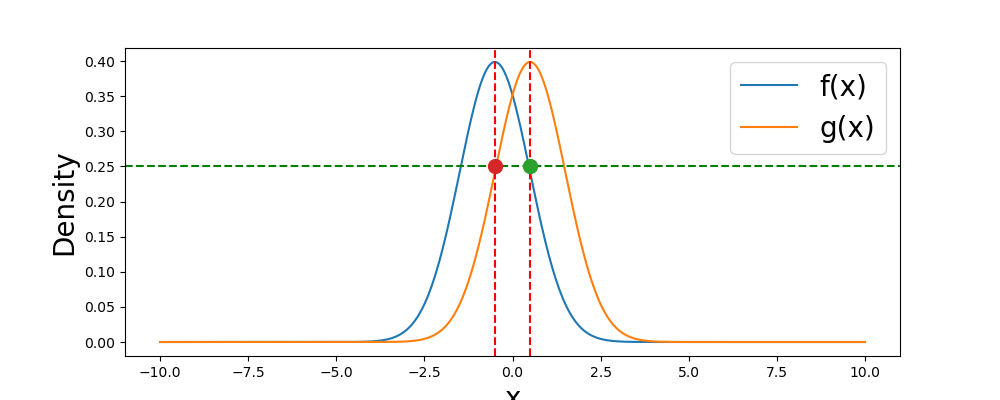
\includegraphics[width=0.8\textwidth]{figures/mcmc_example/proof.png}
    \captionsetup{width=.8\textwidth}
    \caption{Metropolis-Hastings algorithm with symmetric distribution as transition kernel}
    \label{fig:enter-label}
\end{figure}

In this graph, we can see that the green point is the newly sampled point conditioned on the distribution drawn by the last generated point. The red point denotes, on the contrary, the last generated point conditioned on the distribution drawn by the newly generated sample. These two points lie on the same level and share the equivalent value. Thus, the term $\frac{q[Y|X]}{q[X|Y]}$ cancels out to $1$. In this case, the acceptance probability becomes
\begin{align}
\alpha(X, Y) = \min (\frac{\pi(Y)}{\pi(X)}, 1)
\end{align}
which is virtually the ratio of the probability density of the newly generated sample to the probability density of the last generated sample. An illustration of this equation would be as follows: if $\pi(Y) > \pi(X)$, which means that the probability density of the newly generated sample is greater than its of the last generated sample, $\frac{\pi(Y)}{\pi(X)}$ is greater than $1$ and the acceptance of the newly generated point is guaranteed. Over time, the samples that are generated will have greater and greater probability density, and eventually, the peak will be reached. If $\pi(X) > \pi(Y)$, which means that the probability density of the newly generated sample is less than it's of the last generated sample, $\frac{\pi(Y)}{\pi(X)}$ is greater than $1$ and it is still probable to accept the newly generated point, however a less probability that is calculated equation~\cite{understanding_mh}.
\raggedbottom

\section{An example of the Metropolis-Hastings Algorithm}
In this section, an example of the Metropolis-Hastings algorithm will be given and visualized to provide an illustrative comprehension of the different steps of the algorithm. In this example, we want to sample an Erlang distribution from a normal distribution. We are set to generate 100,000 samples to compare how the generated samples fit the Erlang distribution. The Erlang distribution $f(x)$ has a shape of 3 and a scale of 2, whereas the normal distribution $g(x)$ has a mean of 10 and a standard deviation of 1.

\begin{figure}[H]
    \centering
    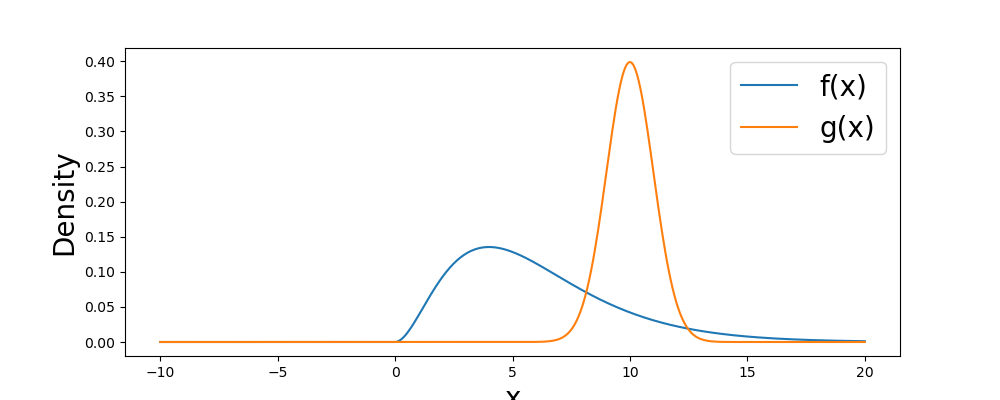
\includegraphics[width=0.8\textwidth]{figures/mcmc_example/first_step.png}
    \captionsetup{width=.8\textwidth}
    \caption{Scaling of the proposal distribution in the Metropolis-Hastings algorithm}
    \label{fig:enter-label}
\end{figure}


As we can see from Figure 2.2, the normal distribution that is sampled does not lie above the Erlang distribution. Therefore, we need to scale up the normal distribution. The scaled up graph is then shown in the Figure 2.3.

\begin{figure}[H]
    \centering
    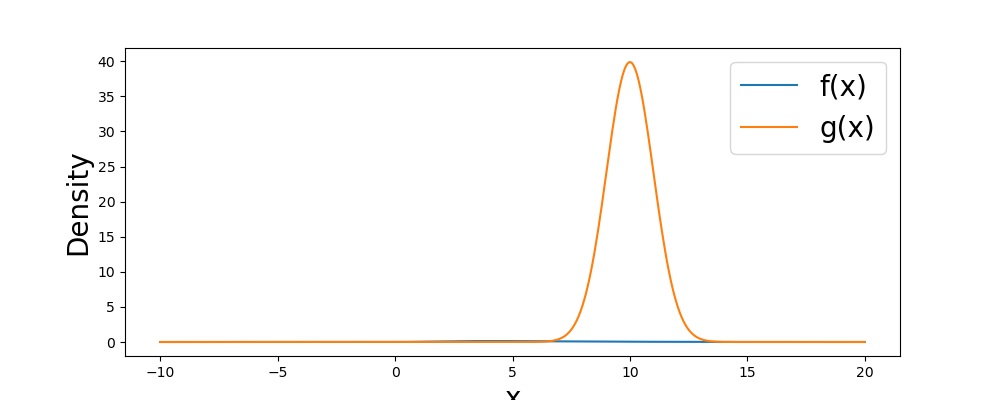
\includegraphics[width=0.8\textwidth]{figures/mcmc_example/second_step.png}
    \captionsetup{width=.8\textwidth}
    \caption{Scaling of the proposal distribution}
    \label{fig:enter-label}
\end{figure}



The transition kernel is set to be a normal distribution that sets the mean as the last generated sample and the standard deviation of 4. Since the normal distribution is symmetric, the acceptance probability could be set to $\alpha(X, Y) = \min (\frac{\pi(Y)}{\pi(X)}, 1)$, as mentioned above. The probability density function of the sampling distribution, $\pi(\cdot)$, is defined as follows:
\begin{align}
\pi(x) = \frac{1}{\sqrt{2\pi} \cdot \sigma}\exp(-\frac{(x-\mu)^2}{2\sigma^2})
\end{align}

where $\mu$ denotes the mean and $\sigma$ denotes the standard deviation of the normal distribution~\cite{densityFunction}.

We select 0 as our starting point and start the iterations from there on. In the first iteration, we acquire the random sample with the value of 1.5437347713886516. The acceptance probability is then $\alpha(X, Y) = \min (\frac{\pi(Y)}{\pi(X)}, 1) = 1$. In this case, since the acceptance probability is 1, it is guaranteed that this sample is accepted. We append this sample to the sample array and move on to the next iteration.

In the next iteration, we sample the value -1.802047900190033. The acceptance probability is then $\alpha(X, Y) = \min (\frac{\pi(Y)}{\pi(X)}, 1) = 0$. This means that this generated sample should by no means be sampled and we should carry on with the last sample. In this case, we repeat our old sample append it to the sample array, and continue.

We continue the rest of the iterations and draw a set of samples. If we plot the samples out and compare them with the target Erlang distribution, it would look something that the graph shown in Figure 2.4. As we can see, the samples that we generate resemble the targeted Erlang distribution. We can conclude that Markov chain Monte Carlo works perfectly in this specific example.

\begin{figure}[H]
    \centering
    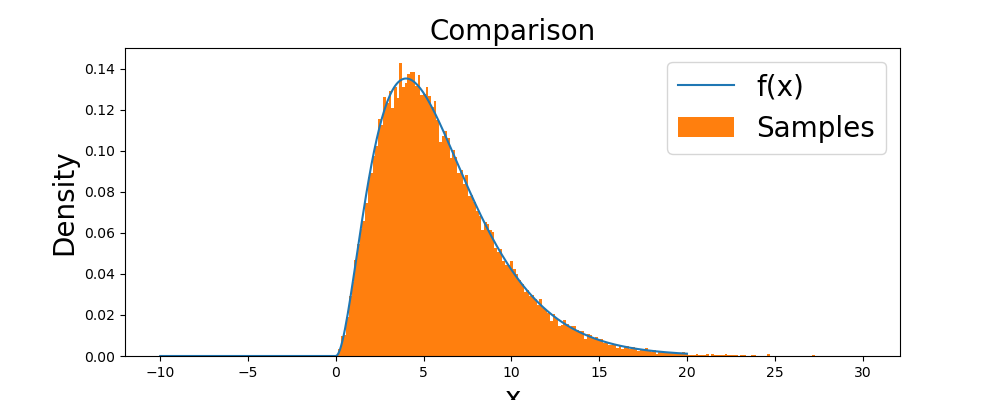
\includegraphics[width=0.8\textwidth]{figures/mcmc_example/result.png}
    \captionsetup{width=.8\textwidth}
    \caption{Posterior distribution derived from the Erlang distribution as proposal distribution}
    \label{fig:enter-label}
\end{figure}

\section{Advantages of Markov Chain Monte Carlo Methods over Other Commonly-Used Sampling Methods}
Markov chain Monte Carlo methods differ from other popular sampling methods and have specific advantages over them. In this section, the rejection sampling and the importance sampling are discussed and are compared to Markov chain Monte Carlo sampling.

Rejection sampling, also known as acceptance-rejection sampling, is a sampling method that generates samples that are independent from one another. Instead of generating the next sample from a newly created distribution that takes the last generated sample as input, the samples are generated from a sampling distribution that lies above the target distribution. The acceptance probability is than the ratio of the density of the target distribution over the sampling distribution~\cite{mcmc_practice}. However, if the target distribution is complicated, especially in multivariate cases, the ratio might be very low, causing the acceptance probability to be low as well, which leads to inefficiency. By creating a dependency between samples, Markov chain Monte Carlo methods avoid this inefficiency~\cite{ComparisonSampling}.

Importance sampling is a sampling method that is based on the calculation of weights. A typical implementation includes the generation of samples, calculating the weights of all of these samples, and calculating the expected value by summing them up together by the weights~\cite{ImportanceSampling}. The process of importance sampling is rather easy to implement. However, a disadvantage is that the samples that have higher weights dominate the calculation of the expected value, which essentially reduces the sample space since the samples that have lower weights play almost no role in the calculation. Markov chain Monte Carlo methods, on the other hand, eventually samples from the stationary distribution after the burn-in period, resulting in consistency of the sampling~\cite{ComparisonSampling}.

\section{The Idea of Parallel Implementation of Markov Chain Monte Carlo}
The objective of this thesis is to implement parallel versions of Markov chain Monte Carlo algorithms for the Bayesian inverse problem. Therefore, paralleling Markov chain Monte Carlo is a significant part of the thesis. The base idea is that instead of one single chain, several chains are run simultaneously~\cite{base_parallel}. Since after the burn-in period, every single state from each chain samples from the stationary distribution due to the ergodic property of the Markov chains~\cite{ergodicity}, all of the samples from different chains could be merged to present the target stationary distribution. However, other variations involve generating multiple points at the same time conditioned on the last generated sample and then evaluating the forward model~\cite{gpmh_broshure}. Since this chapter only provides an overview of the Markov chain Monte Carlo algorithm, a following chapter that is specifically dedicated to the parallel of the algorithm will be given.

\section{Introduction to Bayesian Inference}
The Bayesian inference problem is a method of statistical inference that is used to calculate the probability estimate based on evidence and the likelihood of the set of parameters~\cite{bayesian_inference}. Given a prior distribution that provides information on the preexisting data, the Bayesian inference problem uses the Bayes theorem to update the prior distribution using a likelihood function and derives the actual possibility.

Given the Bayes theorem~\cite{SatzBayes}:
\begin{align}
    \Pr[B|A] = \frac{\Pr[B]\cdot\Pr[A|B]}{\Pr[A]}
\end{align}
where $A$ and $B$ are two different incidents. This equation can than be formed into
\begin{align}
    \Pr[B|A] = \frac{\Pr[B]\cdot\Pr[A|B]}{\int\Pr[B]\cdot\Pr[A|B]dB}
\end{align}
$\Pr[A|B]$ is called the likelihood function, which is generated by a set of data to interpret how likely a particular set of observations is~\cite{likelihood_idea}. The $\Pr[B]$ is called prior, since this is the preexisting knowledge that is given~\cite{prior}. The denominator of the equation is called evidence, which is a constant that depicts the probability of observing the data across all values of the model parameters~\cite{mcmc_practice}. The result of the above equation is the posterior, which is the object of the Bayesian inference problem~\cite{mcmc_practice}.

The different implementations of the Bayesian inference problem are versatile and vary from one another. In this thesis, we implement the Bayesian inference problem using the Metropolis-Hastings algorithm with a normal distribution transition kernel. The idea is that we calculate the acceptance probability based on the posterior calculation. For revision, the acceptance probability of the Metropolis-Hastings algorithm with a normal distribution transition kernel is given by~\cite{mcmc_practice}:
\begin{align}
    \alpha(X, Y) = \min (\frac{\pi(Y)}{\pi(X)}, 1)
\end{align}
Replacing $\pi(\cdot)$ with the posterior distribution, we derive:
\begin{align}
    \alpha(X, Y) = \min (\frac{\Pr[Y]\Pr[X|Y]}{\Pr[X]\Pr[Y|X]}, 1)
\end{align}
In plain language: The acceptance probability is calculated by the ratio of the prior and likelihood of the newly proposed point over the prior and likelihood of the last generated point. Since the evidence is a constant, they cancel each other out and will therefore not be taken into account.

Different variants of implementations are used throughout this thesis to perform Bayesian inference of the hydrological model. They will be discussed in later chapters. For now, we will take a look at the hydrological model.






\chapter{Bayesian Inference and its Use Case in Hydrological Model}

In this chapter, the idea of Bayesian inference will be introduced, including the instantiation of this problem using the Markov chain Monte Carlo algorithm. Afterward, the hydrological model that is used in this paper will be discussed.

\section{Bayesian Inference}
The Bayesian inference problem is a method of statistical inference that is used to calculate the probability estimate based on evidence and the likelihood of the set of parameters.\cite{bayesian_inference} Given a prior distribution that provides information on the preexisting data, the Bayesian inference problem uses the Bayes theorem to update the prior distribution using a likelihood function and derives the actual possibility.

Given the Bayes theorem:\cite{SatzBayes}
\begin{align}
    \Pr[B|A] = \frac{\Pr[B]\cdot\Pr[A|B]}{\Pr[A]}
\end{align}
where $A$ and $B$ are two different incidents. This equation can than be formed into
\begin{align}
    \Pr[B|A] = \frac{\Pr[B]\cdot\Pr[A|B]}{\int\Pr[B]\cdot\Pr[A|B]dB}
\end{align}
$\Pr[A|B]$ is called the likelihood function, which is generated by a set of data to interpret how likely a particular set of observations is.\cite{likelihood_idea} The $\Pr[B]$ is called prior, since this is the preexisting knowledge that is given. The denominator of the equation is called evidence, which is a constant that depicts the probability of observing the data across all values of the model parameters. The result of the above equation is the posterior, which is the object of the Bayesian inference problem.

The different implementations of the Bayesian inference problem are versatile and vary from one another. In this paper, we implement the Bayesian inference problem using the Metropolis-Hastings algorithm with a normal distribution transition kernel. The idea is that we calculate the acceptance rate based on the posterior calculation. For revision, the acceptance rate of the Metropolis-Hastings algorithm with a normal distribution transition kernel is given by:
\begin{align}
    \alpha(X, Y) = \min (\frac{\pi(Y)}{\pi(X)}, 1)
\end{align}
Replacing $\pi(\cdot)$ with the posterior distribution, we derive:
\begin{align}
    \alpha(X, Y) = \min (\frac{\Pr[Y]\Pr[X|Y]}{\Pr[X]\Pr[Y|X]}, 1)
\end{align}
In plain language: The acceptance probability is calculated by the ratio of the prior and likelihood of the newly proposed point over the prior and likelihood of the last generated point. Since the evidence is a constant, they cancel each other out and will therefore not be taken into account.

Different variants of implementations are used throughout this paper to perform Bayesian inference of the hydrological model. They will be discussed in later chapters. For now, we will take a look at the hydrological model.

\section{Overview of the Hydrological Model}
The HBV-SASK conceptual model is a renowned mathematical model that is commonly used in the field of hydrology. HBV is a model that describes the subroutines for snow accumulation and melts, for soil moisture accounting and river routing.\cite{hbv} SASK stands for the province of Saskatchewan, the province in Canada in which the model is developed. The creation of the HBV-SASK model is therefore based on the HBV model but involves local data calibration and integration with local water management needs.\cite{sask}

The HBV-SASK model has twelve different hyperparameters, of which seven are relevant to this thesis. All of these These include:\cite{hydrology}

\begin{itemize}
  \item TT: ranges from -4 to 4, stands for the air temperature threshold in °C for melting/freezing and separating rain and snow
  \item C0: ranges from 0 to 10, describes the base melt factor in mm/°C per day
  \item $\beta$ (beta): ranges from 0 to 3, depicts the shape parameter (exponent) for the soil release equation
  \item ETF: ranges from 0 to 1, describes the temperature anomaly correction in 1/°C of potential evapotranspiration
  \item FC: ranges from 50 to 500, depicts the field capacity of soil in mm.
  \item FRAC: ranges from 0.1 to 0.9, stands for the fraction of soil release entering the fast reservoir
  \item K2: the slow reservoir coefficient ranges from 0 to 0.05, which determines what proportion of the storage is released per day
\end{itemize}

To run this model, these hyperparameters need to be determined. Since the only prior information given is the lowest and the highest bound of each hyperparameter, uncertainty quantification of these hyperparameters is, therefore, necessary to gain posterior information. Apart from these hyperparameters, the starting and the end date of the period that is used for uncertainty quantification are also required to be specified. However, the very first phase at the start is used for the spin-up phase, in which the model runs for some time using historical data. This phase stabilizes internal model states such as soil moisture and groundwater levels, which are important for accurate simulation.
TODO: states

\section{Overview of the Data Set}
There are two existing data sets to the hydrological model, which are respectively called Oldman Basin and Banff Basin, since they are each measured at the Oldman River and in the town of Banff in Alberta, Canada.\cite{hydrology_dataset} The value that is measured is called streamflow. It describes the movement of water within a river or stream channel and is the combined result of all climatological and geographical factors that operate in a drainage basin.\cite{streamflow} Both of these data sets are presented in the format of a time series, in which the value of each measurement is collected against the dates over a long period. The Oldman basin data set is available from 1979 to 2008, whereas the Banff basin data set is available from 1950 to 2011.\cite{hydrology}

Since the data is presented in a format of time series, a time series decomposition is required to present more information on trends, and seasonal and regression effects.\cite{time_series} After the decomposition, the trend, seasonal, and residue of the dataset over the whole period can be observed. For the time series decomposition in this section, the function TSA.seasonal.seasonal\_decompose from the python framework stats models is used.\cite{stat_models_decompose}

First, we take a look at the result of the decomposition of the Oldman basin data set.
\begin{center}
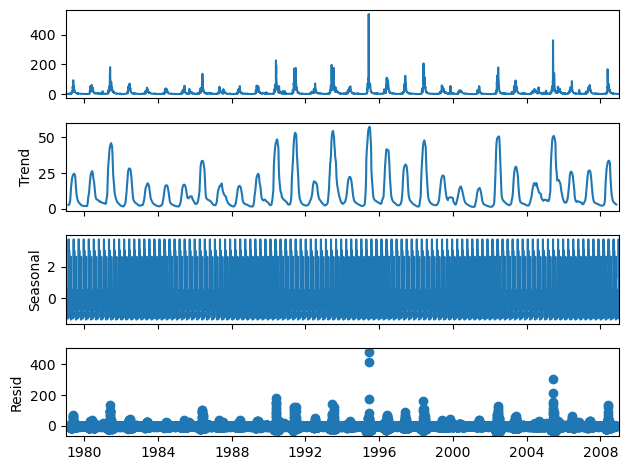
\includegraphics[width=0.8\textwidth]{figures/dataset_time_series/Oldman.png}
\end{center}
The seasonal component of this time series is regular over the years. However, there were significant peaks around the early 1980s, mid-1990s, and around 2005. The streamflow in these periods is higher than anytime else, which indicates that there might be possible heavy rainfalls, floods\cite{hydrology}, or even ecologic disasters. Anomalies in this period can be also found in the residue component, which confirms that there might be odd behaviors happening in these periods. Therefore, quantifying the uncertainty of these three periods would be a challenging task.

We then take a look at the result of the decomposition of the Banff basin data set.
\begin{center}
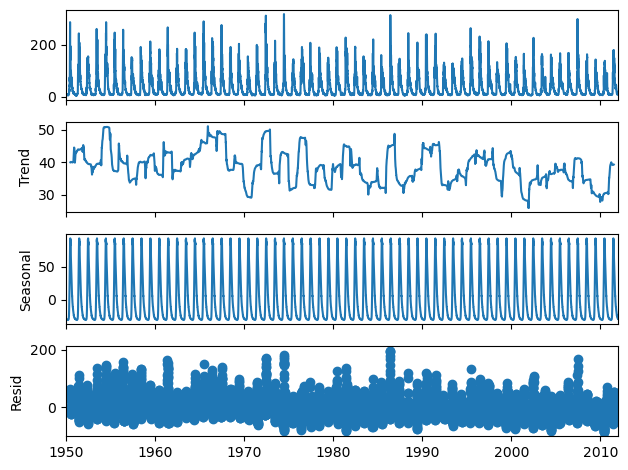
\includegraphics[width=0.8\textwidth]{figures/dataset_time_series/Banff.png}
\end{center}
Similar to the case of Oldman Basin, it shows a regular seasonal component. The trend, on the other hand, fluctuates across the entire measured period but does not show a general upward or downward direction. This means, that the whole measurement is indeed relatively stable. However, the fluctuation might still impose an influence on the accuracy and stability of uncertainty quantification. The residuals of the Banff basin data set are much more varied than the Oldman basin data set. There are obvious clusters of high activity and anomalies, which confirms that the uncertainty quantification of this data set might be a hard task to deal with.


\section{Task}
Since the task of this paper is to quantify the uncertainty of the input parameters of the hydrology model, the process is therefore as follows: First, the model is created with the configuration of the period and target distributions being given. Then, we select an appropriate Markov chain Monte Carlo algorithm and perform sampling to solve the Bayesian inference. In this process, the output of each generated set of parameter arrays will be calculated by the model. The output will be later compared to the measured data points, which will provide the algorithm with an acceptance rate. In each iteration, the algorithm decides whether to accept or reject this sample. Last but not least, we collect all the samples and perform analysis.

To test the generalized application of the algorithm, we select three challenging yet representative periods for testing, with one being long (5 years), another being medium long (around 2 years) and the other being short (1 year). Due to the constant fluctuation of the Banff basin data set, we could select a long period within it to perform uncertainty quantification. Since the residue in the early 1970s seems to show extreme anomalies, we select 1970 to 1975. The other two periods are both picked from the Oldman Basin data set. The period from 1994 to 1996 is chosen, since there are apparent anomalies of the residue in this period. Another period is the year 2005, since there are also anomalies being showcased in this year.

\chapter{Fundamental Implementation}
In this chapter, a basic version of Metropolis-Hastings is implemented. Complications including the parallel aspect, more complicated algorithms, and further enhancement are not considered in this chapter. A general idea of the implementation is explained, with specific sections contributing to possible issues with the general algorithm and the choice of the likelihood function.

\section{Hardware Specification and Required Frameworks}
All of the code that is run and tested in this paper is run on a single computation machine, namely the MacBook Pro 2021 by Apple Inc. It has an Apple M1 Pro chip, which has an ARM architecture. It has 10 CPU cores, 8 of which are for performance and the rest are for efficiency. It has a RAM of 32 GB and also 16 GPUs available\footnote{https://support.apple.com/en-us/111902}. The entire code is run on macOS Sonama 14.4.1.

The software implementation of the fundamental Metropolis-Hastings algorithm is rather basic. Since the sample space is multivariate, the calculation involves operation between vectors. To ease the process of these calculations, the popular software package of Numpy is used.\cite{numpy} Additionally, the Tensorflow Probability package is used. It does not only offer implemented probability distribution functions, but also randomness and sampling functions.\cite{tfp} To use the Tensorflow Probability framework, the software package Tensorflow is required to be installed\footnote{https://www.tensorflow.org/probability}. For the visualization part, standard data visualization libraries including Matplotlib and Seaborn are used for the creation of histograms, kernel density estimation, and boxplots.\cite{plt}

\section{Basic Metropolis Hastings and Evaluation Metrics}
First of all, we take a look at the basic implementation of the Metropolis-Hastings algorithm. This implementation applies the idea of the algorithm mentioned in the chapter above. It takes the following required input parameters: the proposal distribution that data points are sampled from, the sampling kernel for transition, the likelihood kernel for calculation of the likelihood and acceptance rate, the initial state where the algorithm starts, and the number of iterations. Since the prior distributions of the parameters that are going to be calibrated are normal, the boundaries need to be given as input parameters, so that the algorithm can examine whether the generated samples are out of bounds, which should be ignored. The sampling kernel that is used throughout this paper is the Gaussian normal distribution since it provides symmetry and simplicity.\cite{gaussian_distribution_property} The concrete algorithm goes as follows.

\begin{algorithm}[H]
\SetKwFunction{BasicMetropolisHastings}{MH}
\SetKwProg{Fn}{Function}{:}{}
\KwIn{\tabto{2cm}proposal distribution, sampling kernel, likelihood kernel, initial state, iterations}
\KwOut{\tabto{2cm} sampled data points}
\BlankLine

\Fn{\BasicMetropolisHastings{arr}}{
    \tcp{Extract parameters}
    [proposal\_dist, sampl\_kernel, likel\_kernel, init\_state, iterations] = arr\\
    samples \leftarrow [init\_state]
        
    \For{i $\leftarrow$ 0 \KwTo iterations - 1}{
        \tcp{Calculate probability}
        old \leftarrow samples[-1]\\
        new \leftarrow sampl\_kernel(old)\\
        p \leftarrow proposal\_dist(new) * likel\_kernel(new) / (proposal\_dist(old) * likel\_kernel(old))\\
        \tcp{Decide to accept or reject the sample}
        \If{random $>$ min(1, p)}{
            samples.add(samples[-1])
        } \Else {
            samples.add(new)
        }
    }
    \Return samples
}

\caption[Metropolis Hastings]{Basic Metropolis Hastings}
\end{algorithm}

There are two required kernels for the input parameters, namely the sampling kernel and the likelihood kernel. The sampling kernel, as mentioned above, acts like the transition of the Markov chain between two consecutive samples. It plays a critical role in the performance and results of a Markov chain Monte Carlo simulation.\cite{mcmc_practice} Due to the ease and efficiency of calculation that is discussed above, symmetric distribution, notably normal distribution, is used in this paper.\cite{gaussian_distribution_property} However, the shape of the kernel is left unknown and is to be determined by the standard deviation.\cite{normal} The choice of the standard deviation is crucial. If the standard deviation is too wide, the generated samples will keep getting out of bounds. If the standard deviation is too narrow, it will take too long time to explore the whole distribution range, because it is more likely that the new sample generated is near the mean. 

The likelihood kernel also plays a crucial role in the Markov chain Monte Carlo. It measures the probability of observing the data given the set of the generated parameters under the model.\cite{likelihood_general} In this paper, the likelihood function for the kernel is implemented as a normal distribution probability function due to the Central Limit Theorem, which suggests that the mean of a large amount of independent random variables will be approximately normally distributed regardless of the underlying distribution.\cite{central_limit_theorem} In other words, the normal distribution describes the noise of the data points around the mean, which is the sampled value. The likelihood function of the Gaussian normal distribution is given by the product of all of the probability densities of each point:\cite{gaussian_likelihood}
\begin{align}
    L(\mu, \sigma^2; x_1, ..., x_n) = \prod_{j=1}^n \frac{1}{\sqrt{2\pi}\sigma} e^{-\frac{(x_j-\mu)^2}{2\sigma^2}}
\end{align}

Given that the calculation process is numerically hard to solve, the log-likelihood function is commonly used.\cite{log_likelihood} The log-likelihood function of the Gaussian normal distribution is given by:\cite{log_gaussian_likelihood}
\begin{align}
    \log[L(\mu, \sigma^2; x_1, ..., x_n)] = -\frac n 2\ln(2\pi\sigma^2) - \frac 1 {2\sigma^2}\sum_{j=1}^n (x_j - \mu)^2
\end{align}
 
Both of these above equations are implemented as help functions in this thesis for easier further applications. However, an easier way of implementation is to use a probability modeling framework to create a multivariate normal distribution centered around the given value, calculate the likelihood for each pair of points, and sum them up together. This version is also implemented using the TensorFlow probability library and is mainly used throughout this thesis. The only unknown thing is the standard deviation of the distribution. Similar to the sampling distribution, the standard deviation is a left-to-be-determined variable that describes the shape of the distribution. In the context of the likelihood function, the standard deviation implies how concentrated the data are expected to be around the mean value.\cite{standard_deviation_estimation} A smaller standard deviation suggests that the data points are expected to cluster tightly around the mean and have less tolerance, whereas a larger standard deviation implies a broader spread of data points and more tolerance. 

Using the above-listed algorithm, we can perform Bayesian inference on the HBV-SASK model. Because the calibrated parameters in the HBV-SASK model are seven-dimensional instead of one-dimensional, the acceptance rate is, therefore, a seven-dimensional array. In this case, to represent the generality of the acceptance rates given by each parameter, the mean of the entire array is taken as the final acceptance rate. There is also an option of taking the maximum value from the array, but the selection will be discussed later in the section of "Input Parameter Exploration".

To quantify the accuracy mathematically, we need to introduce metrics that can calculate the accuracy of the Bayesian inference results. First, we calculate the mean of the absolute difference between the calculated time series run by the model and the measured time series. By calculating the absolute difference, the similarity of the times series could be well quantified. Afterward, two metrics that are used to test the goodness of fit are calculated, namely root mean square error (RMSE) and mean absolute error (MAE). The RMSE is a metric that is often used to evaluate the model performance in climate research studies and ecology. The calculation is as follows: 

\begin{align}
\text{RMSE} = \sqrt{\frac 1 n \sum_{i=1}^n (y_i - \hat{y_i})^2}
\end{align}

The square root in RMSE plays an important role. On the one hand, RMSE penalizes larger discrepancies more severely by squaring the errors.\cite{RMSE_discrepency_penalty} Moreover, it helps to stabilize the variance of the error terms, making it particularly useful in the use case of this paper, since the usage of standard deviation and variances are present in the implementation.\cite{RMSE_MAE}

The MAE is another widely used metric for model performance evaluation.\cite{RMSE_MAE} 

\begin{align}
\text{MAE} = \frac 1 n \sum_{i=1}^n |y_i - \hat{y_i}|
\end{align}

Calculating the average of absolute errors means that it is easier to understand and interpret the calculation directly. Besides, due to the less impact of anomalies on the metric,\cite{RMSE_MAE} MAE can offer a more robust estimate in contexts when extreme values are expected to be anomalies.

The whole process of evaluation of the results is going to look like this. 
To collect this result, we first randomly generate 1000 samples from the given posterior using the Monte Carlo simulation \cite{monte_carlo_simulation} and take the mean. The results of the calculation are saved as "posterior mean". Calculating the mean value, which generalizes the entire results, would allow us to observe the actual accuracy of the result since every single individual time series contributes to the calculation process. Next, the maximum value of each timestamp is also found, so that we can observe how extreme the posterior samples could be. The result is then saved as "posterior max", which would indicate how stable the sampling process is. If the posterior max does not differ much from the posterior mean, then the entire sampling space is stable. Otherwise, the individual samples vary too much from each other, causing destabilization. These two time series are then compared to the "prior mean" time series, which is the mean of all the calculated time series of the model that takes samples from prior as input, to observe how much the prior distribution influences the result. After calculating all of the above, a visualization is going to be done so that these results can be compared to each other. 

For simplicity, we only use the Oldman Basin dataset for training purposes in this paper. For the exploration phase, the model will be run and evaluated on the same training dataset, so that we can observe how well the trained posterior fits the data on which it is trained. For the actual evaluation, the model will be run on the training dataset, whereas the accuracy score will be evaluated from a testing data set, which is a year 2005 of the Oldman Basin dataset.

Apart from the accuracy test, efficiency also plays an important role in the MCMC algorithms.\cite{MCMC_efficiency} To test the efficiency, the run times of different implementations are going to be recorded, so that a comparison can be done later and we can infer which factors have impacts on the computation time.

Another thing that needs to be done is to select meaningful values or instances to be input parameters. In the following sections, we are going to discuss the choices of input parameters based on two methods. First, the input parameters are going to be selected using existing knowledge. Afterward, the input parameters are going to be explored, in which models with different input values are going to be run multiple times. Afterward, the accuracy tests that are mentioned above are going to be carried, out so that an overview of the relation between different input parameters and the accuracy and efficiency result can be visualized. An overview of which set of input parameters delivers the best overall accuracy and efficiency is also going to be shown later on. To test how well the posterior fits the data on which it is trained, the evaluation part is going to be carried on the training data as well. In the end, the sets of input parameters from both methods are going to be used for another run of the algorithm, so that the results of the Bayesian inference problems can be compared with each other. The evaluation, however, is going to be carried on on the testing data, so that we can observe how well the posterior would perform in actual cases.

\section{Visualization}
After deriving the results, visualization helps us to understand the data well, regardless of posterior distributions or relations between input parameter configurations and accuracy. 

For the use case of the Bayesian inference problem, two types of visualizations are necessary. First, we need to know how the individual parameter distributes in the posterior probability. The result of the Metropolis-Hastings is a multidimensional list of values, representing the calculated posterior. For each parameter, a separate histogram is generated. Alongside the histogram is the Kernel Density Estimation (KDE) graph. It is used to estimate the probability density function of a random variable based on a data sample by averaging contributions from specific kernel functions that are centered at each data point.\cite{kde} By combining the histogram and the KDE graph, an overview of the general distribution of the posterior can be understood.

However, if the histogram and the KDE plot resemble the prior distribution, little or no useful information can be retrieved. Therefore, we can visualize the data using boxplots to get specific information on the distributions of the posterior of each parameter. The data we can read from the boxplot are the locations of different samples so that we can know how many samples are located under the first quantile, above the third quantile, or the median. It provides us with an easier understanding by explaining the locations of all of the samples in the posterior distribution.

After considering these parameters individually, we regard all of the parameters as a whole. In this case, we investigate whether specific parameters create dependency on each other. To deal with this, a heatmap is plotted, which shows the correlation of each pair of parameters. If the two parameters are too highly correlated, it would be possible that the samples of one parameter are dependent on another parameter. In this case, decoupling is needed to prevent entanglement, so that each parameter can sample on its own without the influence of other parameters.

At the very end of the parameters visualization, the calculated results are going to be compared. The four times series including posterior mean, posterior max, prior mean and measured data, which are mentioned before, are going to be plotted on the same graph so that the results can be visually compared.

The other type of visualization is presented during the exploration phase of the input parameters. The charts present the relations between the input parameter configurations and the metrics results. If the configuration is the form of numeric values, the line plot is drawn, so that a possible existing trend could be detected. If the configuration contains categorical values, then a bar chart is drawn instead. By plotting the metrics against the configuration, a clear comparison of the results calculated by different sets of input parameters is provided.

\section{Knowledge-Based Input Parameter Selection}

Before exploring the model's input parameters, we can determine the input parameters by logic previous knowledge, and logical thinking. In this section, the Bayesian inference problem will be directly executed, as well as the visualization part. First, all different input parameters are going to be individually discussed.

The proposal distribution is, for the use case of the hydrological data set, relatively straightforward. Since there is no further information regarding the shape and look of the distribution other than the upper and the lower bound, a multivariate uniform distribution that ranges from the lower and the upper bound could be modeled and used as the proposal distribution.

The determination of the standard deviation of the sampling kernel is crucial to the result of the algorithm. Since the standard deviation should generally not be a bigger value than $\frac 1 4$ of the range,\cite{good_standard_deviation} we start to find a maximum value of the factor going down from there so that the transition kernel of the algorithm does not go out of bounds too often, which causes numerical errors. After several test runs of the model, we found out that the first appropriate sampling kernel is a normal distribution with the standard deviation set as $\frac 1 6$ of the range, since it is neither too wide nor too narrow, which allows the algorithm to run smoothly and effectively reduce the amount of sampling out of bounds. This value is thus set as the default standard deviation.

The default standard deviation value is set to $1$. The intention of setting the standard deviation to a relatively low value is to expect better precision. Since normal distributions with narrow standard deviations give out lower probabilities if the value is away from the mean, the samples that are far away from the mean will receive more penalties, if the standard deviation is set low. This results in a lower likelihood value, which might lead to a lower acceptance probability.

For the rest of the attributes: The initial state does not affect the accuracy of the result\cite{mcmc_practice}. Therefore, it is set as a random set of values within the uniform distribution for now. To increase the random effect, we generate 1000 random samples and take the mean as the random result. Optimization for efficiency is going to be performed later in this paper. For now, we simulate the Bayesian inference problem using Markov chain Monte Carlo for 10.000 iterations. As suggested, $20$ percent of the data are discarded due to the burn-in phase.\cite{20per_burnin}


We execute the algorithm with the above-suggested input parameters. The execution was successful and produced decent results. Several graphs are produced to provide a great visualization of the result. 

First, we take a look into the posterior distribution of individual parameters. The graph is shown in Figure 4.1. As we can see from the histogram and the KDE plot, the calculated posterior does not resemble specific distributions. They share a similarity, that is the probability of samples near the boundaries are relatively lower than the samples near the center. All of these parameters also have several peak values, which are sampled in the posterior distribution more than other values. All of the values are relatively widespread and evenly distributed. 

Since little information is gathered from the above plot, we can visualize the data using boxplots to get specific information on the distributions of the posterior of each parameter. As we can see from the boxplots that are shown in Figure 4.2, the boundaries of the posterior distributions are retained. They share the same boundaries as the prior distribution. However, the first and third quantile as well as the median of the posterior distribution. This gives us a general idea of how the posterior would look like. For further application of Markov chain Monte Carlo algorithms, the starting values could potentially be altered based on this information to improve efficiency. This aspect will be discussed later in this chapter.


\begin{figure}
    \centering
    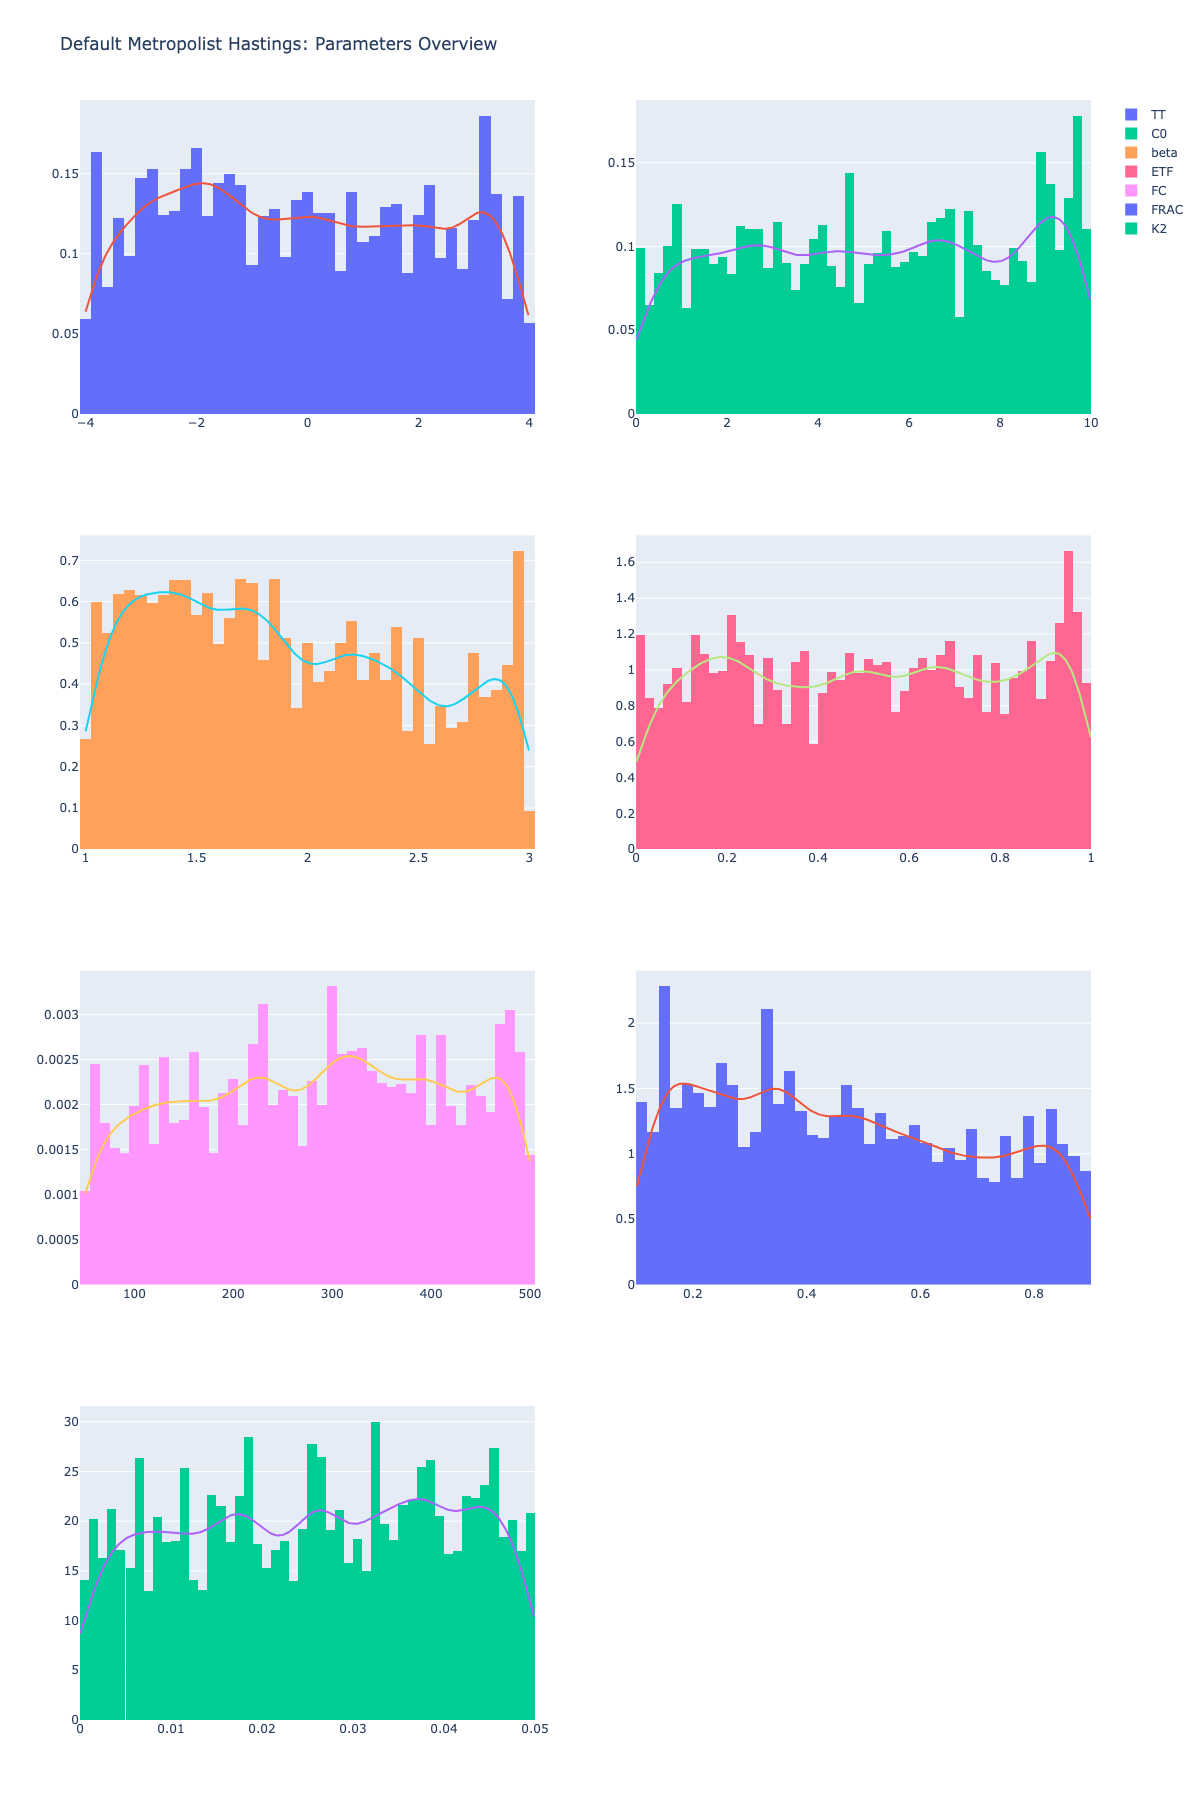
\includegraphics[width=1\textwidth]{figures/basic_mh/default_mh/default_mh_parameters_overview.png}
    \captionsetup{width=.8\textwidth}
    \caption{Overview of the posterior distribution of the parameters calibrated by the default Metropolis Hastings algorithm}
    \label{fig:enter-label}
\end{figure}



\begin{figure}
    \centering
    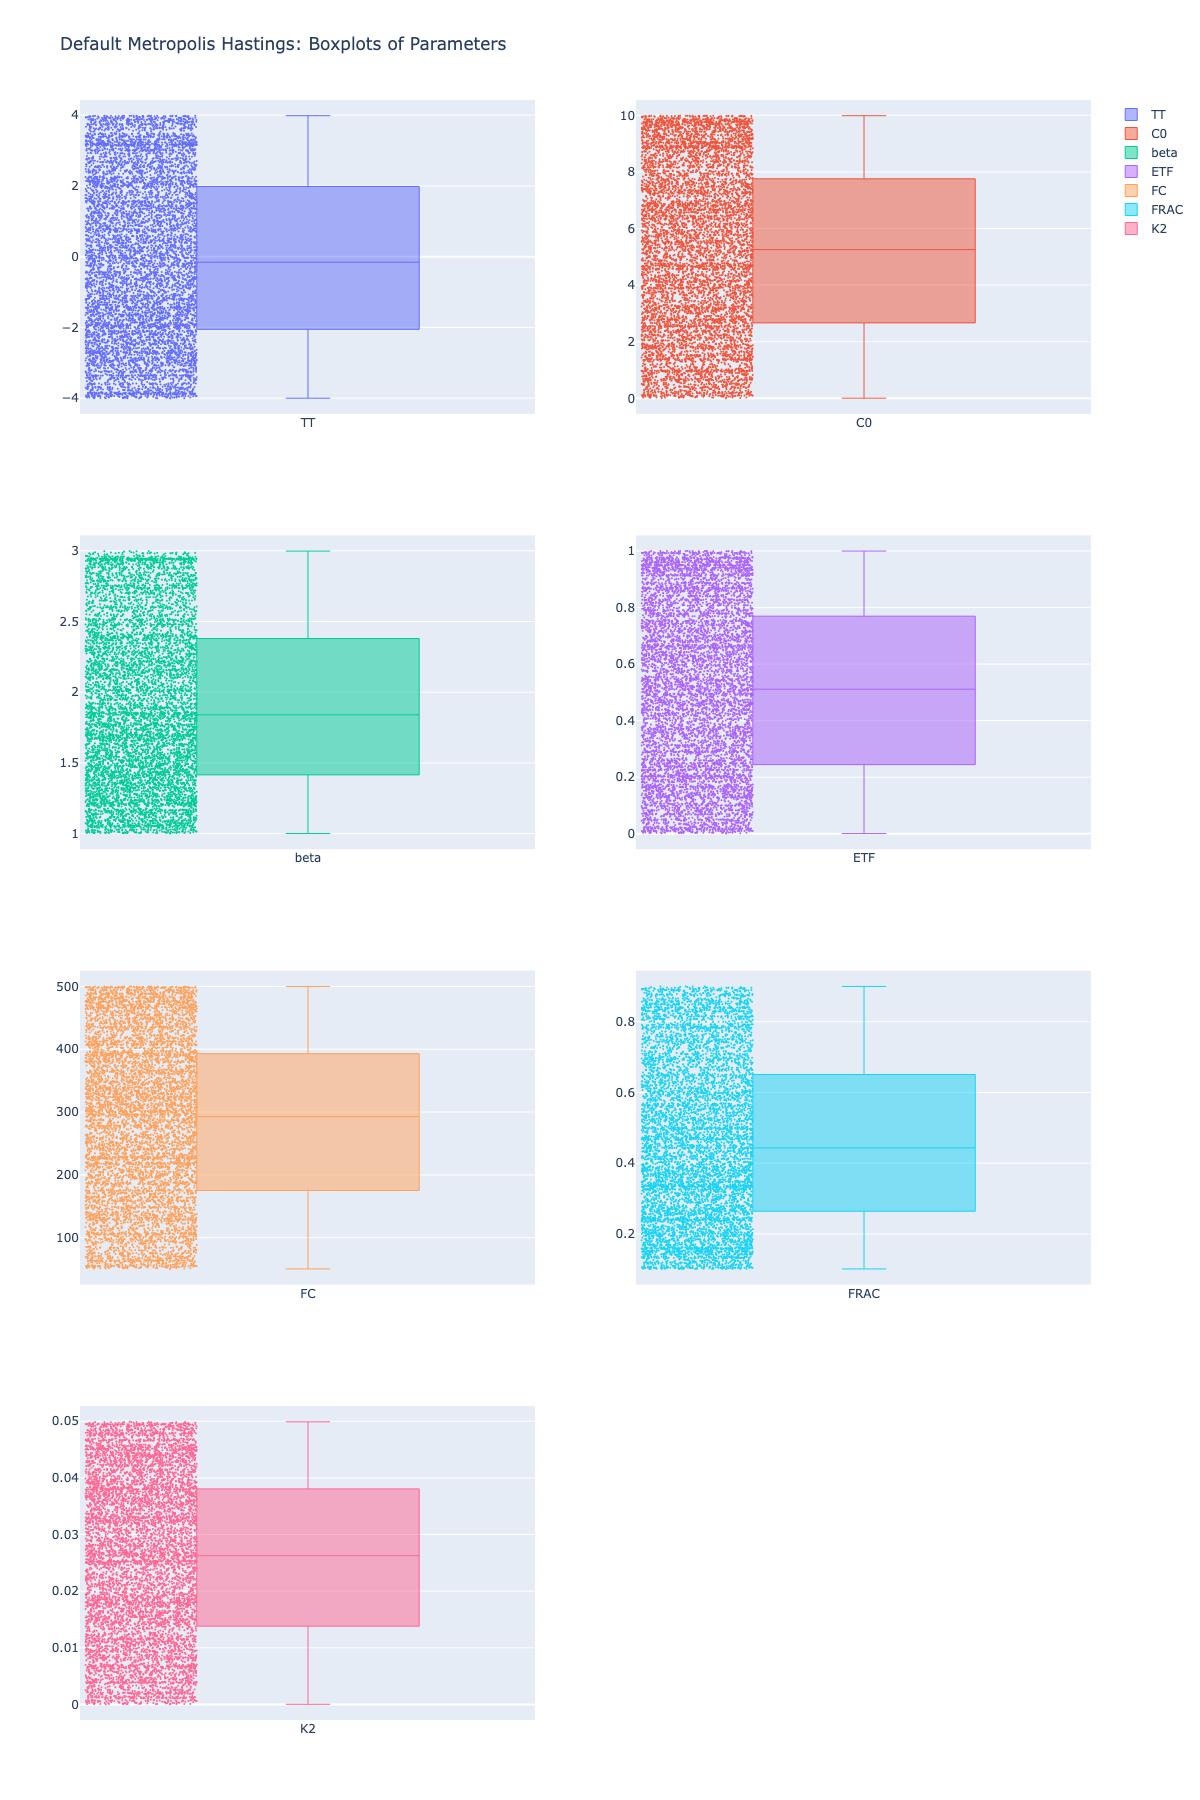
\includegraphics[width=1\textwidth]{figures/basic_mh/default_mh/default_mh_boxplot.png}
    \captionsetup{width=.8\textwidth}
    \caption{Boxplots of the generated posterior samples of each parameter calibrated by the default Metropolis Hastings algorithm}
    \label{fig:enter-label}
\end{figure}



After considering these parameters individually, we regard all of the parameters as a whole. In this case, we investigate whether specific parameters create dependency together using the heatmap. From the heatmap shown in Figure 4.3, we can see that none of the parameters are strictly dependent on each other. Specific pairs of parameters such as TT and FC do share more or less level of dependency, nevertheless, these are extremely low so this factor can be neglected. In this case, no specific changes to the likelihood functions need to be made.


\begin{figure}
    \centering
    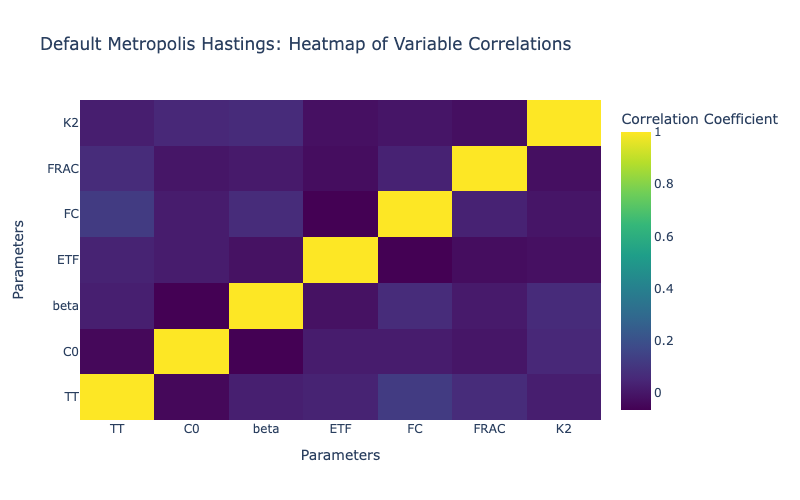
\includegraphics[width=1\textwidth]{figures/basic_mh/default_mh/default_mh_heatmap.png}
    \captionsetup{width=.8\textwidth}
    \caption{Heatmap between parameters that are calibrated by the default Metropolis Hastings algorithm}
    \label{fig:enter-label}
\end{figure}


After analyzing the parameters individually and as a group, the result that is computed by the posterior of the Bayesian inference is revealed in Figure 4.4 and compared to the observed data. The calculated result resembles the actual measured data, particularly the posterior mean. It reaches its peak in the same period as the measured data, whereas it shows stable behavior for the rest of the time, just like the the measured data. The posterior max shows slightly more extreme behaviors at certain points. Both of the posterior time series show significant improvement based on the prior mean. 


\begin{figure}
    \centering
    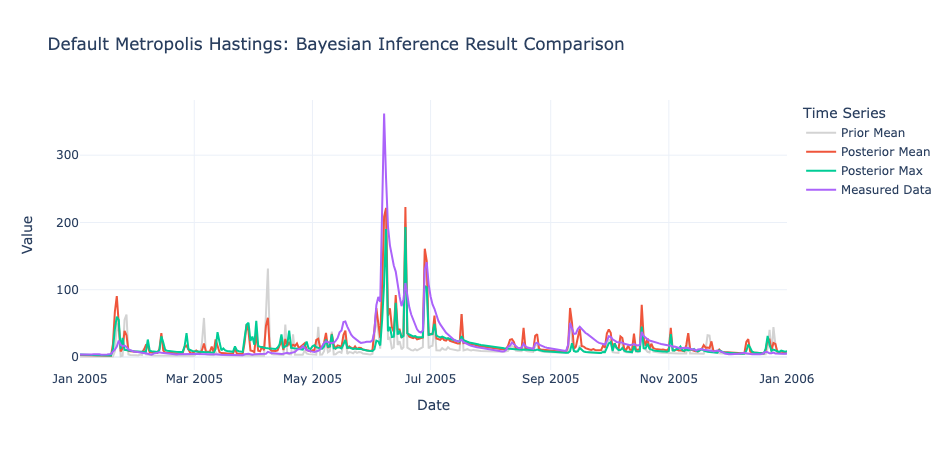
\includegraphics[width=1\textwidth]{figures/basic_mh/default_mh/default_mh_bayes.png}
    \captionsetup{width=.8\textwidth}
    \caption{Comparison of Bayesian inference results of the default Metropolis Hastings}
    \label{fig:enter-label}
\end{figure}

After visualizing the parameters, we take a look at the accuracy of the data. For this part, the RMSEs and MAEs are calculated. The RMSE of the posterior mean is 22.14475485613421 and the MAE of the posterior mean is 11.399487080387862. From the graph, we can see that a significant difference in the results is shown around the peak, which might contribute to the relatively high MAE and a decent value of RMSE. The RMSE of the posterior max is 26.72454579307846 and the MAE of the posterior max is 13.196081237340492. They do not show too many differences from the posterior means, which means that the posterior distribution is relatively stable. 

However, these values currently mean nothing, as they will be compared later to the results after the input parameters exploration. In the following sections, we are going to explore specific parameters of the Metropolis-Hastings algorithm to achieve maximum accuracy. Besides, the efficiency will also be taken into account, where the run time of the algorithm will be observed and compared.


\section{Input Parameters Exploration}
After finding the appropriate values by knowledge-based selection, all of the input parameters will be explored in this section. By trying out different reasonable values as input and interpreting the accuracy and efficiency results, we might be able to figure out a specific relation between the different input values against the accuracy or the efficiency score. Later on, the algorithm will be run using the set of input parameters which delivers the best performance by accuracy and efficiency metrics and be compared with the input parameters by knowledge-based selection on the testing data.

\subsection{Sampling Out of Bounds}
While executing this algorithm for the hydrological model, however, there is a certain issue. Since no specific information regarding the distribution is given, we are required to use the uniform distribution to describe the parameters that need to be calibrated. Since the uniform distribution ranges from a certain lower bound to a certain upper bound, it does not have an unlimited range. In this case, there is a possibility that the newly generated samples are out of bounds, which is not helpful for the calibration. For example, if a generated point, which is accepted, is out of bounds, the $p$ variable in the algorithm will be set to 0, which causes invalid values like negative infinity to occur in the calculation. If these values are sampled and carried on, values that are further from the bounds may be going to be sampled, which leads to mistakes in the result. Therefore, measures need to be taken to avoid these errors from happening. Three implementation variants against this issue have come up. These are ignoring, boundary aggregation, and reflecting boundary.

The ignoring method is the default method and the most straightforward: Any points that are generated outside of the bound are going to be eliminated since they are seemingly useless for the sake of uncertainty quantification. It is extremely important to mention that instead of taking another sample from the iteration, the last generated sample needs to be carried on. Since the sample out of bounds is supposed to be an impossible case, the acceptance rate in that point needs to be treated as 0, which means that this point is directly rejected. For multivariate distribution, a set of data points needs to be rejected entirely at once if one single data point is out of bounds since the acceptance rate otherwise would be different. Otherwise, the detailed balanced condition could be violated, as the transition probabilities would not be symmetric anymore for every single parameter.

The boundary aggregation method is different in treating the out-of-bounds samples, in which it transforms the sampled data that are out of bounds. Instead of reflecting the data that is out of bounds, we simply sample the upper bound or the lower bound and carry on from there. If a new sample is generated based on the normal distribution that is centered around the out-of-bounds sample, there is less or equal to fifty percent chance that the newly generated point is inside the range.\cite{gaussian_distribution_property} The main benefit of this method is that there is still a minimum of fifty percent chance that the next sample is kept inside the bound in cases where the samples are out of bounds. For multivariate distribution, a single data point in each dimension can be handled individually, however, the acceptance rate needs to be calculated based on the transformed sample points. 

The posterior that is derived from the boundary aggregation method is shown in Figure 4.5.  A few samples are getting aggregated on both sides of the boundaries. If we ignore these two bars on both sides, the distributions of the rest of the samples of each parameter still resemble uniform distributions, which does not provide a lot of information regarding the actual distribution of the parameter. 

The boxplot of these samples is shown in the Figure 4.6. An obvious takeaway from this chart is that all of the boxplots have a lower first quantile and a higher third quantile, whereas the median is retained almost at the same place. The disposition of both of these quantiles is the result of the aggregation of samples on both sides of the boundaries.


\begin{figure}
    \centering
    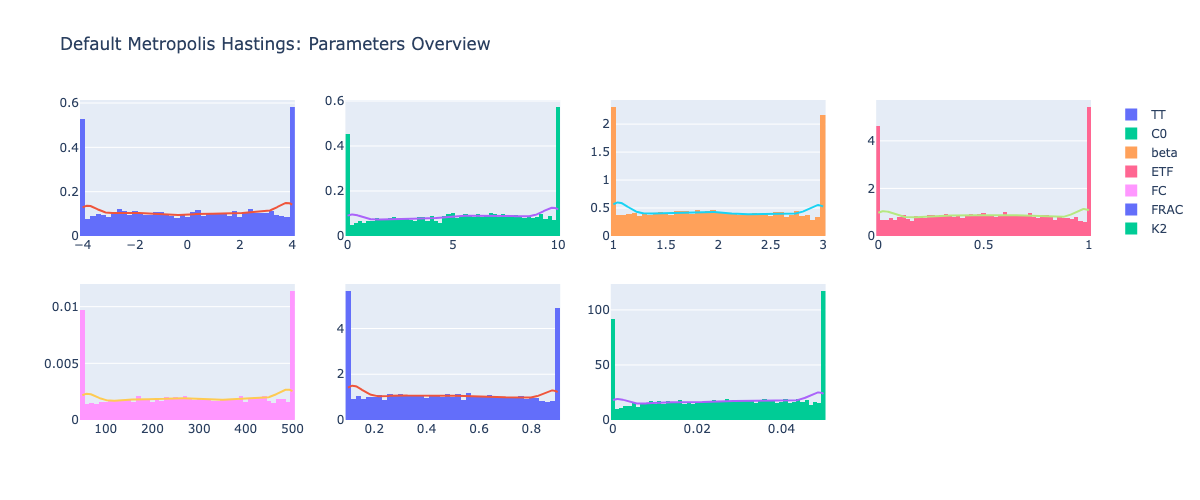
\includegraphics[width=1\textwidth]{figures/basic_mh/aggr_mh/aggr_mh_parameters_overview.png}
    \captionsetup{width=.8\textwidth}
    \caption{Overview of the posterior distribution of the parameters calibrated by the Metropolis Hastings algorithm that samples the bound value if the sample is out of bounds}
    \label{fig:enter-label}
\end{figure}

\begin{figure}
    \centering
    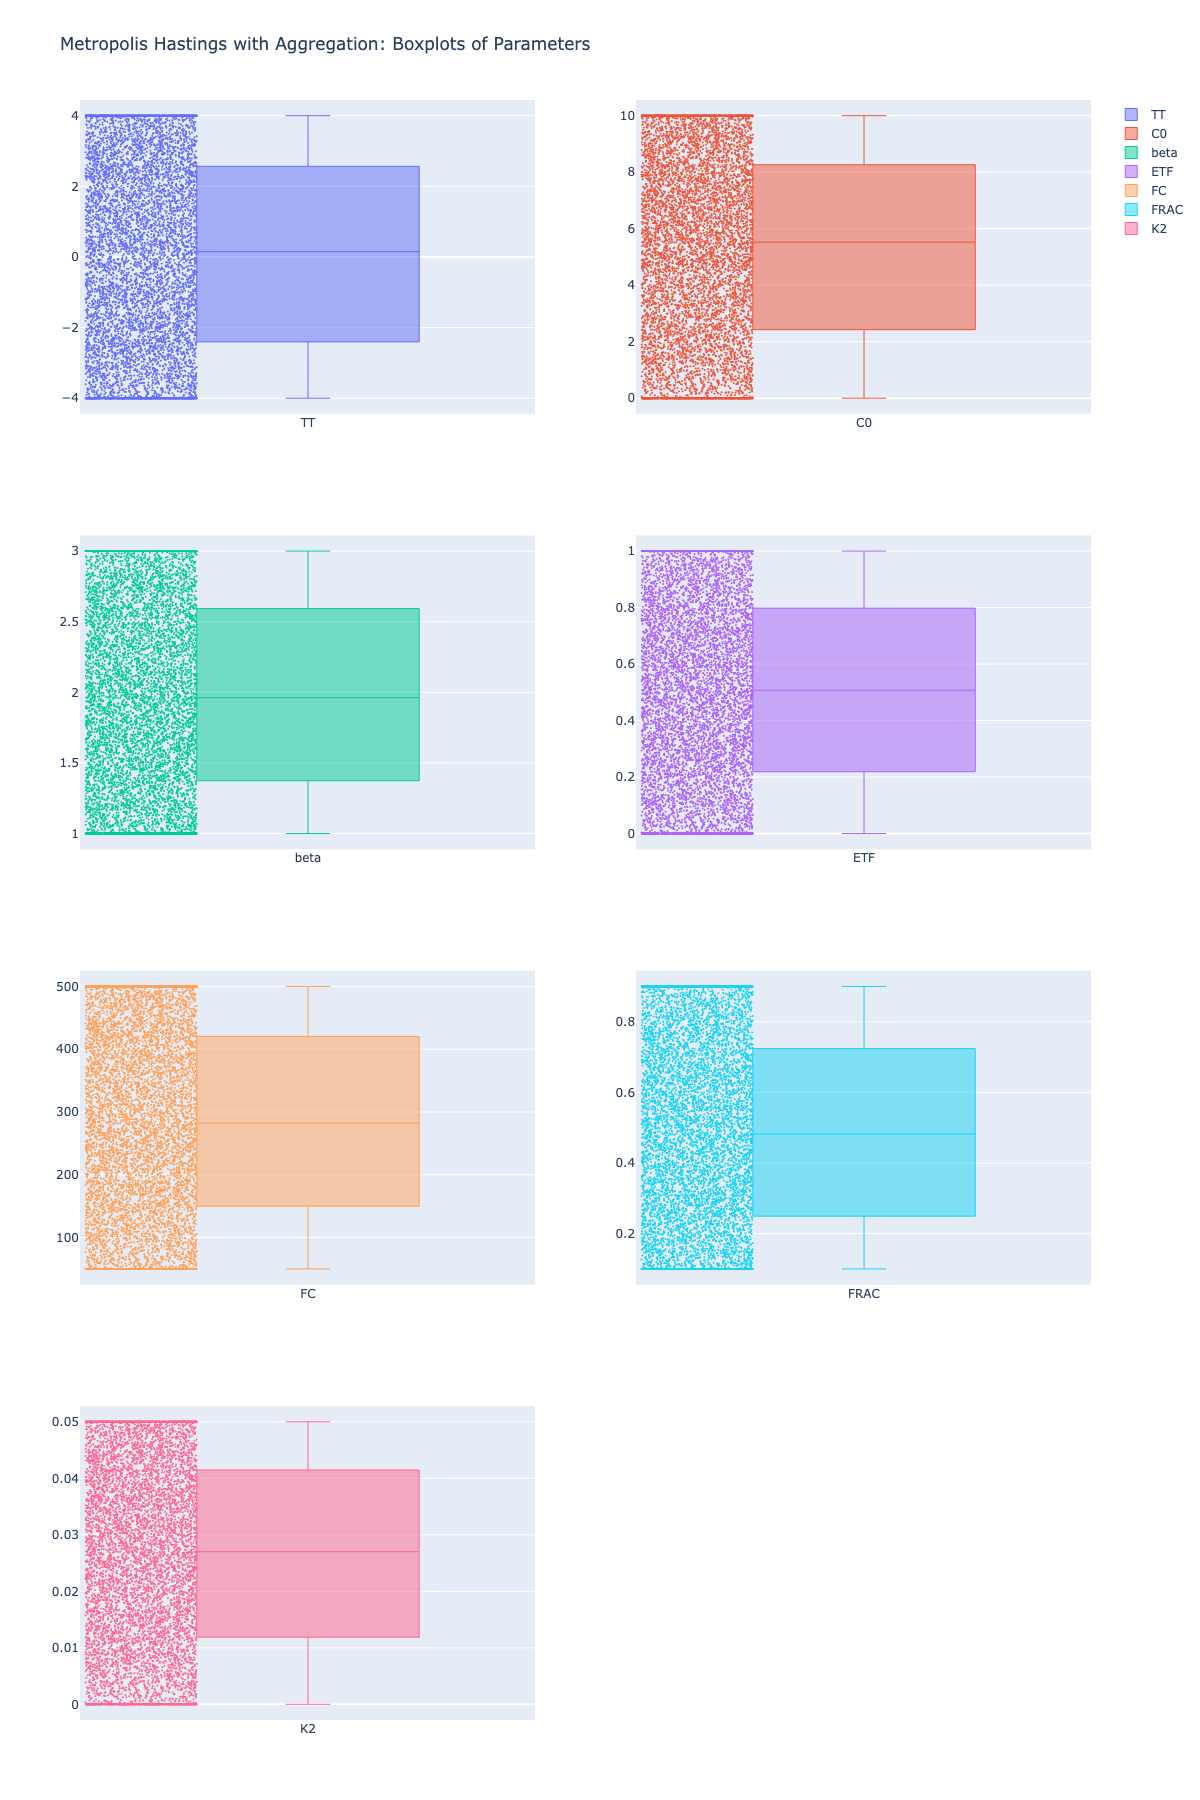
\includegraphics[width=1\textwidth]{figures/basic_mh/aggr_mh/aggr_mh_boxplot.png}
    \captionsetup{width=.8\textwidth}
    \caption{Boxplots of the generated posterior samples of each parameter
calibrated by the Metropolis Hastings algorithm that samples the bound value if the sample is out of bounds}
    \label{fig:enter-label}
\end{figure}



The reflect boundary method also transforms the data instead of ignoring it but in a different way than the aggregation method. Due to the symmetry of the transition kernel, the possibility of sampling an out-of-bounds sample is the same as the possibility of sampling the point symmetric over the mean of the Gaussian normal transition kernel.\cite{gaussian_distribution_property} In this case, the acceptance rate of the transformed sample point is not changed, which has no interference with the algorithm itself and future samples. For multivariate distribution, a single data point in each dimension can be handled individually and the acceptance rate does not need to be recalculated due to the symmetry of the transition kernel distribution. 

We now take a look at the posterior distribution of the samples. It is shown in Figure 4.7. From the graph, we can see that the posterior distributions sampled from this version of Metropolis-Hastings look very much different from the others. All of these posterior distributions resemble normal distributions, with one peak somewhere in the middle. For some parameters like C0, beta, ETF, and TT, the boundary is shifted, which means that no samples from the region near the boundaries are generated. Since all of the samples that are out of bounds are reflected, the reflected samples compensate the holes of the nonreflected samples, so that it gives rise to a normal distribution like posterior.

\begin{figure}
    \centering
    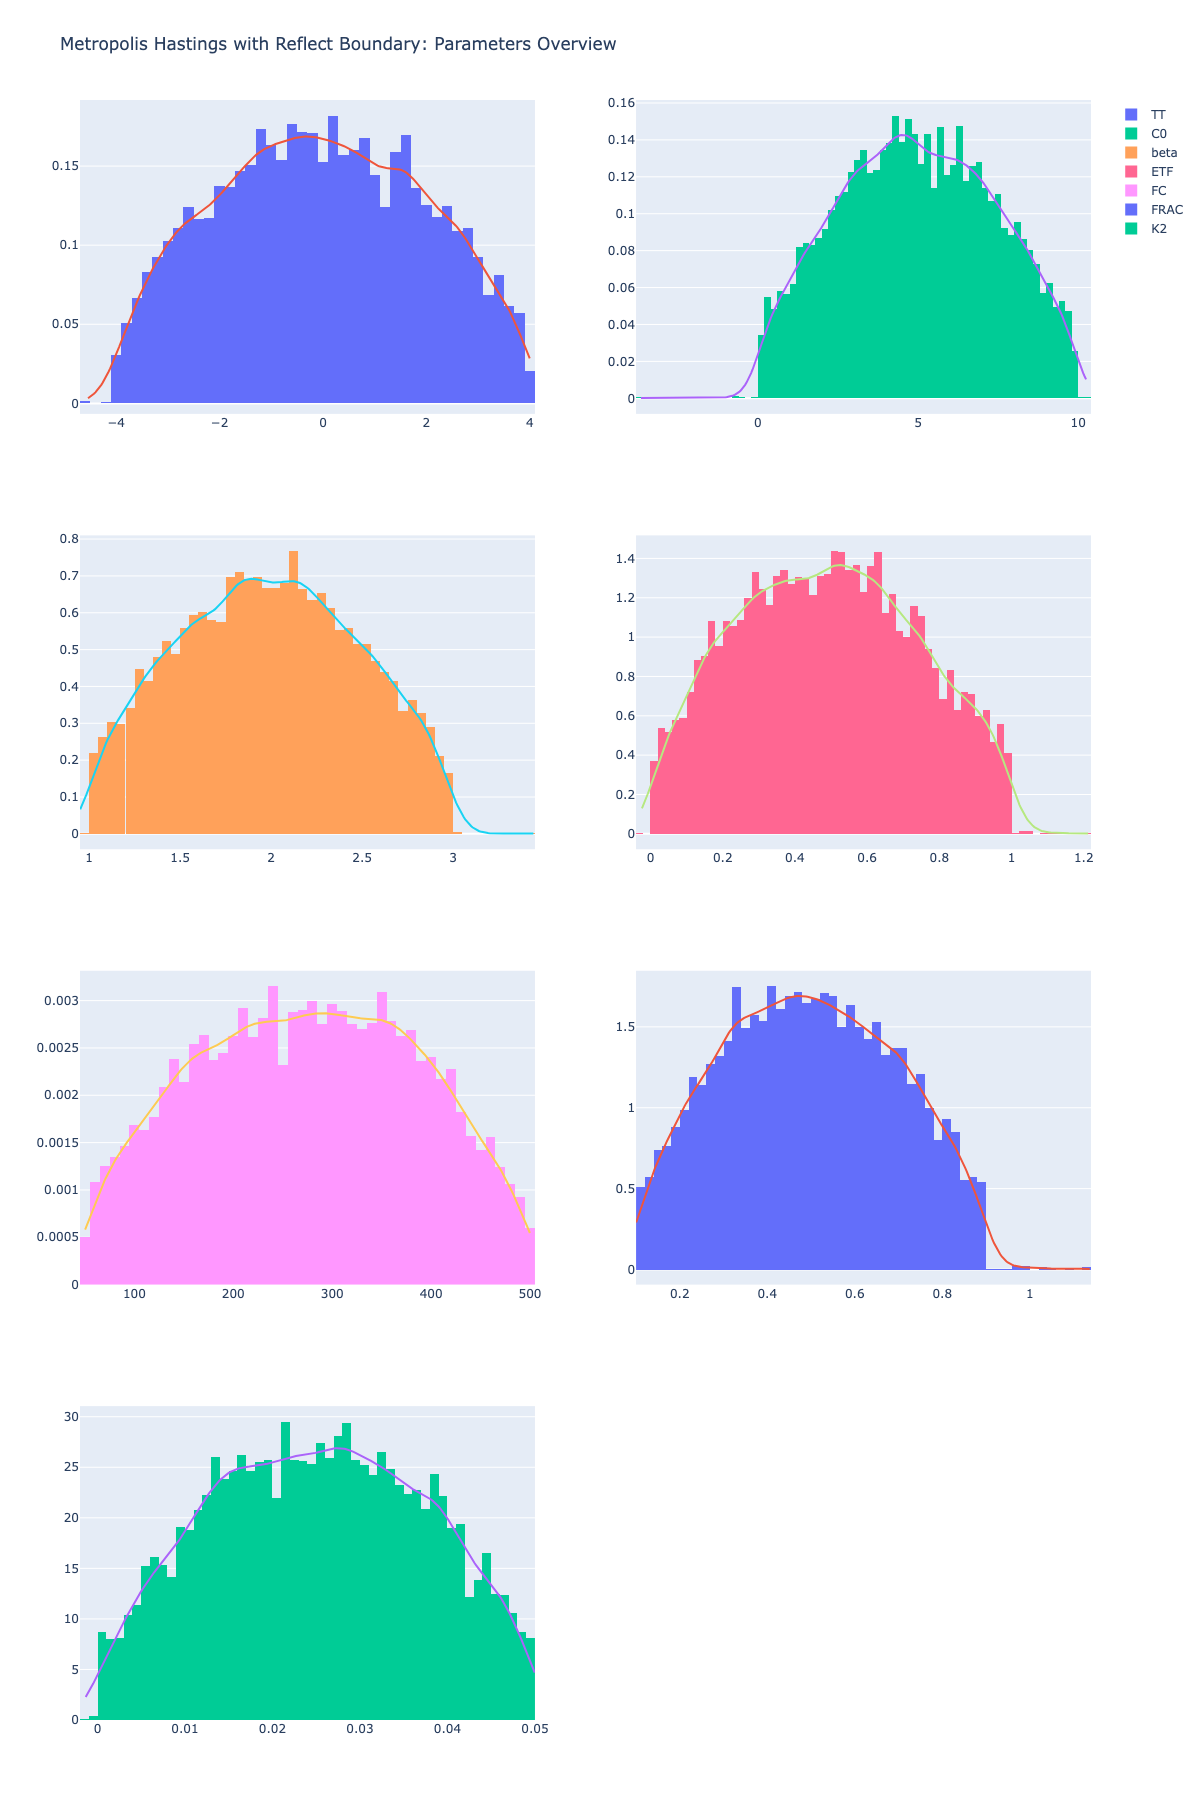
\includegraphics[width=1\textwidth]{figures/basic_mh/rb_mh/rb_mh_parameters_overview.png}
    \captionsetup{width=.8\textwidth}
    \caption{Overview of the posterior distribution of the parameters calibrated by the Metropolis Hastings algorithm that reflect the samples into the inside of the range if the they are out of bounds}
    \label{fig:enter-label}
\end{figure}

The boxplots of the parameters are shown in Figure 4.8. Due to the normal distribution like posterior, all of the boxplots shrink by a certain amount, with some having lower upper bounds or upper lower bounds. This is an apparent result, since the shape of the normal distribution focuses on the mean, whereas the sampling probabilities of samples that are further from the mean are lower. This property can be presented by the boxplots.

\begin{figure}
    \centering
    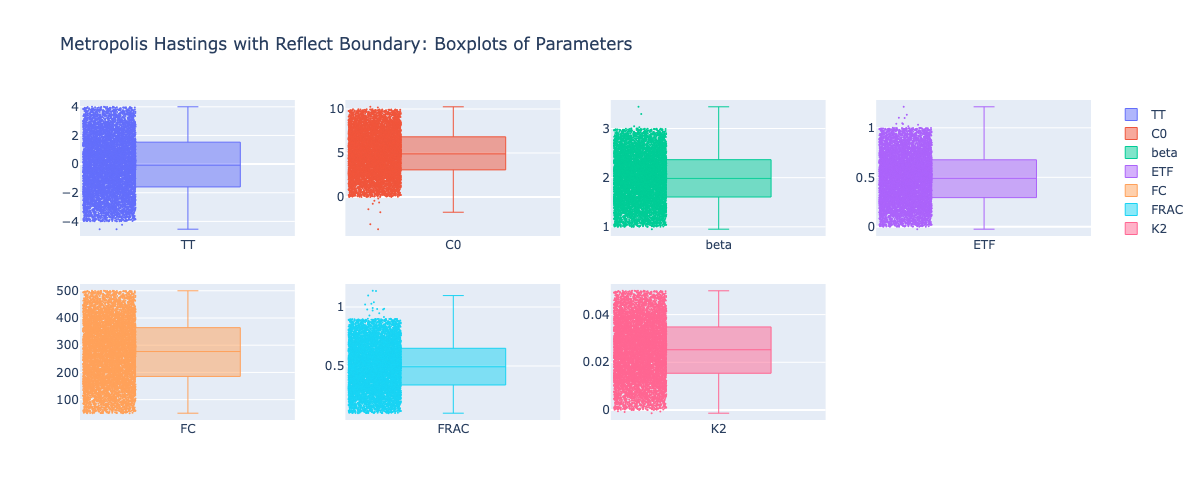
\includegraphics[width=1\textwidth]{figures/basic_mh/rb_mh/rb_mh_boxplot.png}
    \captionsetup{width=.8\textwidth}
    \caption{Boxplots of the parameters calibrated by the Metropolis Hastings algorithm that reflect the samples into the inside of the range if the they are out of bounds}
    \label{fig:enter-label}
\end{figure}



To find out which of these three variants delivers the best result, each of these three versions is separately executed, while all of the rest input parameters are set to the same value or instance. The different metrics that are mentioned in the section above are then calculated and visualized using a bar chart so that the values can be compared. 

The result is shown in Figure 4.9. The first impression of the bar chart is that the accuracy of the actual inferred results is pretty similar among all three versions, with the ignoring and the aggregate methods performing only slightly better. For efficiency, however, the ignoring performs better than both of the other methods by a huge margin. The reason behind it is obvious: the ignoring operation is way more efficient than the reflecting boundary and aggregation, which involves mathematical operations. Therefore, the default ignoring method is the clear winner here and should be retained for further model executions.


\begin{figure}
    \centering
    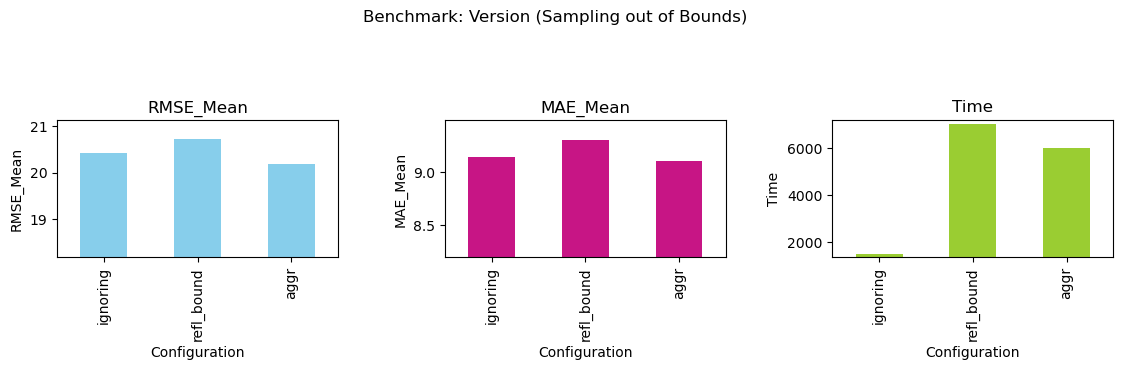
\includegraphics[width=0.8\textwidth]{figures/basic_mh/benchmark/sampling_otb.png}
    \captionsetup{width=.8\textwidth}
    \caption{Comparison of the accuracy and the efficiency of different Metropolis Hastings algorithms}
    \label{fig:enter-label}
\end{figure}



\subsection{Sampling Kernel}
The sampling kernel plays a crucial role in the accuracy and efficiency of the performance. Since we stick to the normal distribution in this paper, the standard deviation is the only value that needs to be explored. As suggested, the default value of the standard deviation is set to $6$ because it is the largest possible number that fits in the use case of the hydrology model. However, the final result would also be different if the standard deviation is less than the optimal one. In this case, the movement of the samples is going to be relatively centered local, since the points in the vicinity of the mean are more likely to be sampled. To test multiple scenarios and their behaviors, three values for the standard deviation are going to be tested in the following execution: the range interval over $8$, over $10$, over $12$, over $18$, and over $24$.

\begin{figure}
    \centering
    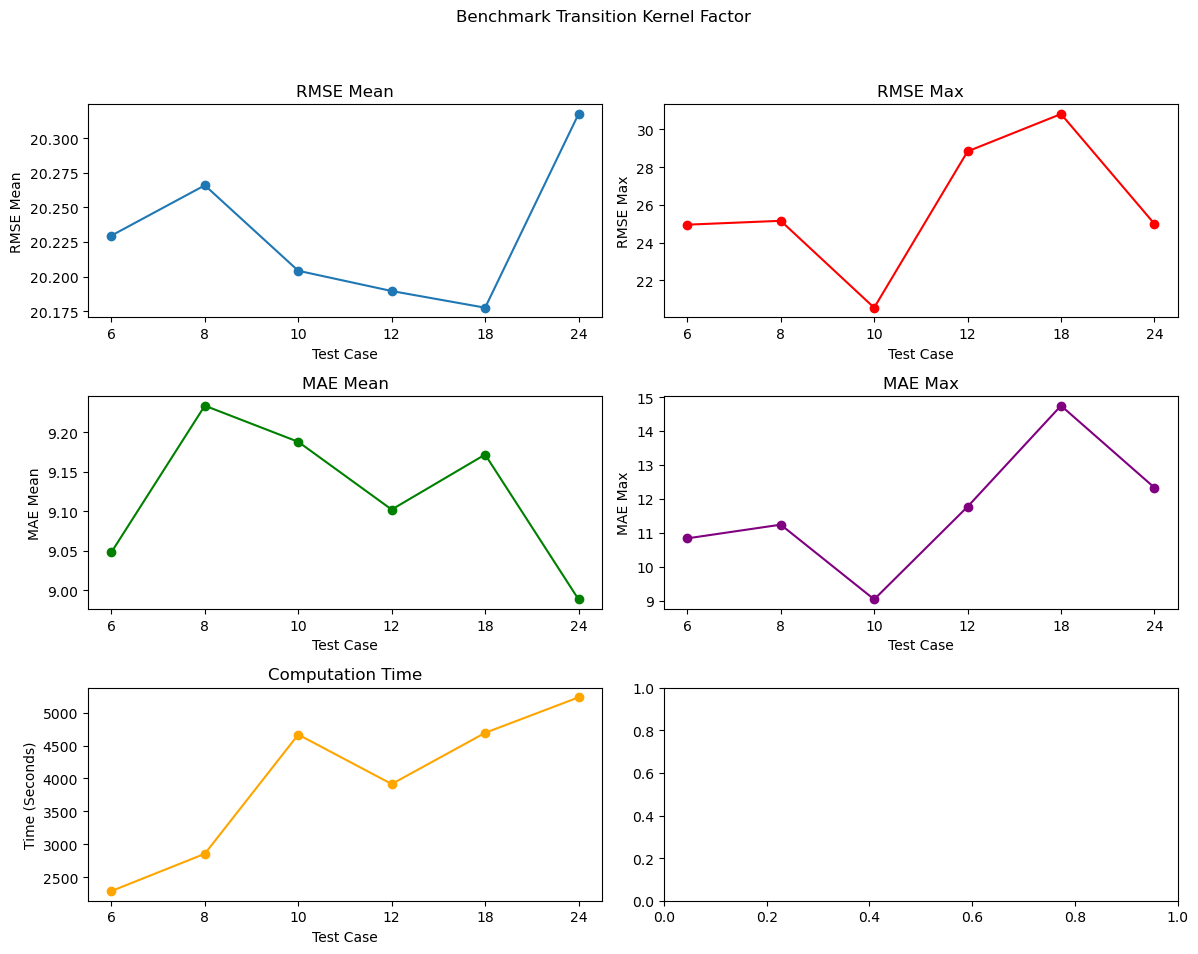
\includegraphics[width=0.8\textwidth]{figures/basic_mh/benchmark/sensitivity_transition.png}
    \captionsetup{width=.8\textwidth}
    \caption{Comparison of the accuracy and the efficiency of Metropolis Hastings algorithms based on the sampling kernel standard deviation}
    \label{fig:enter-label}
\end{figure}

TODO

\subsection{Likelihood Functions}
At the start of the chapter, we have already discussed the importance of the role played by standard deviations in the likelihood functions. As mentioned before, $1$ is selected for the default value. However, the choice of the standard deviation does impact the final result, since it exerts an influence on the sampling probability of the values based on their distance from the mean. If the standard deviation is set lower, the sample that is away from the mean will receive less probability. If the standard deviation is set higher, that sample will not receive that little probability, which allows more tolerance to be present in the calculation. However, the value cannot be too large, otherwise, the tolerance level will be too high for the likelihood function to give out a meaningful solution. Thus, for the test values, we go down from $1$ down to $8$, which is an interval of values that still might generate meaningful calculations. The selected values for testing are $1$, $3$, $5$ and $8$. 

As we can derive from Graph 4.11, the metrics for the mean also do not differ that much from each other. In this case, the conclusion could be drawn that the standard deviation does not have a huge impact on the actual inferred result. For the inferred maximum time series, the discrepancy is also not obvious, even though the test case $5$ shows the most instability throughout the posterior. Nevertheless, using the test case $5$ results in the most efficient calculation, whereas using the test cases $1$ and $2$ will require slightly more computation time.


\begin{figure}
    \centering
    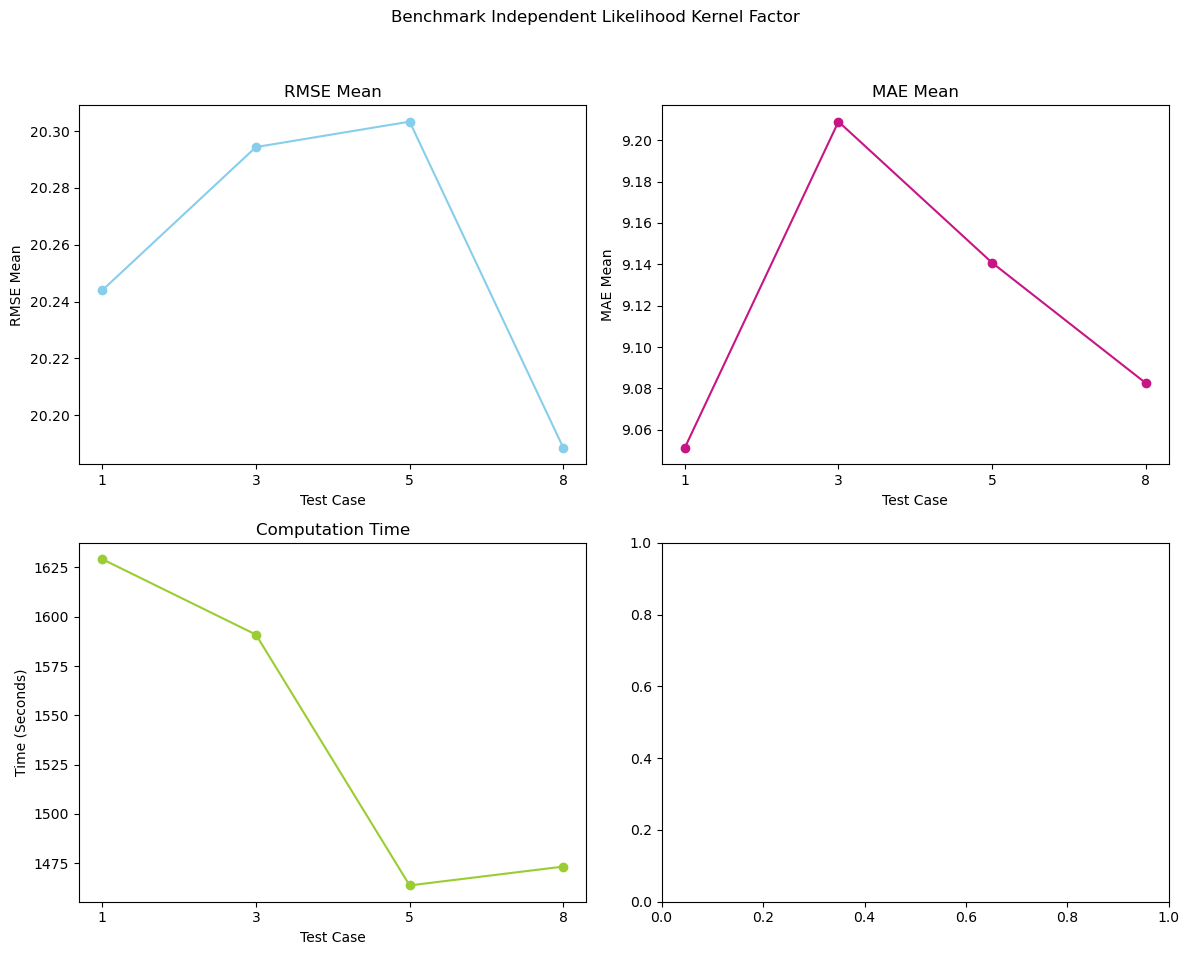
\includegraphics[width=0.8\textwidth]{figures/basic_mh/benchmark/sensitivity_likelihood_independent.png}
    \captionsetup{width=.8\textwidth}
    \caption{Comparison of the accuracy and the efficiency of Metropolis Hastings algorithms based on the likelihood function standard deviation}
    \label{fig:enter-label}
\end{figure}



The above-computed likelihood function takes in a value as the standard deviation so that each sample is independently observed from another. However, this standard deviation can potentially be even more optimized if the standard deviation is based on some value that is meaningful for the final calculation. If there is somehow a correlation between the likelihood function and the observed data, which provides an absolute exact value, we might derive the information regarding the correlation between the inferred data and the observed data, so that the calculated likelihood could be more precise. Therefore, we introduce here the dependent likelihood function, which takes in the observed data as the standard deviation. Since the observed data might be too large for the likelihood function to deliver meaningful results, an alternative way is to take a certain factor of the observed data as input. Here, several factors are going to be tested, including $0.2$, $0.4$, $0.6$ and $0.8$. The goal is to observe the correlation between the accuracy and the value as it increases.


The result is shown in Figure 4.12, where we can see a pattern: the accuracy of the inferred data decreases as the factor increases. As for the computation time, the case of $0.6$ requires the most time to perform computation, and is, however, still pretty similar to the rest. Therefore, the case $0.2$ should be the optimal choice.

\begin{figure}
    \centering
    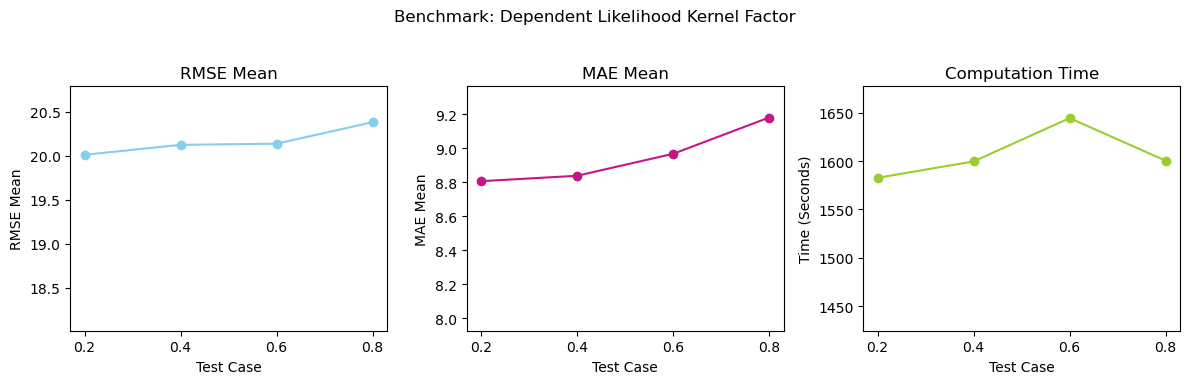
\includegraphics[width=0.8\textwidth]{figures/basic_mh/benchmark/sensitivity_likelihood_dependent.png}
    \captionsetup{width=.8\textwidth}
    \caption{Comparison of the accuracy and the efficiency of Metropolis Hastings algorithms based on the dependent likelihood function standard deviation}
    \label{fig:enter-label}
\end{figure}


Comparing the dependent and the independent version of the likelihood functions, the dependent version with a standard deviation of $0.2$ times the measured data outperforms the independent version with a standard deviation of $5$, despite a slightly longer run time, which is reasonable due to the mathematical computation of the standard deviation. The incorporation of exact data in the likelihood function does provide a more accurate result.

\subsection{Alternative Implementation of Probability Acceptance Rate}
After we explore both of the input parameters that are responsible for the calculation of the acceptance rate, we move on to the selection of the acceptance rate. Due to the multi-variate property of the HBV-SASK model, the calculated acceptance rates will be formed into an array. To transform this array into a value, there are two choices: One option is that we take the mean of all the values as an acceptance rate, so that the final acceptance rate could more generally represent all of the individual acceptance rates by parameter. Another option is to take the maximum value of the entire acceptance rate array. On the one hand, we can improve the efficiency of the algorithm, since the calculation of the mean is avoided. On the other hand, some dimensions might be easier to sample from than others due to less complexity. Using the maximum acceptance rate gives us therefore the insight of the entire parameter space, where the parameter with the best performance decides the acceptance rate. However, the maximum acceptance rate might be misleading if the distribution of the acceptance rate array is too widespread, which results in the complete opposite of efficiency and accuracy.

We execute the algorithm in both versions, with the rest of the parameters being identical. Graph 4.13 suggests that for the HBV-SASK model, the mean sampling method does not only deliver a slightly better performance in accuracy but also more stability and most importantly: better efficiency. This shows that the acceptance rate in each iteration in the array might have far different values so the max sampling method cannot deliver good enough results. Therefore, we stick to the original mean sampling method.


\begin{figure}
    \centering
    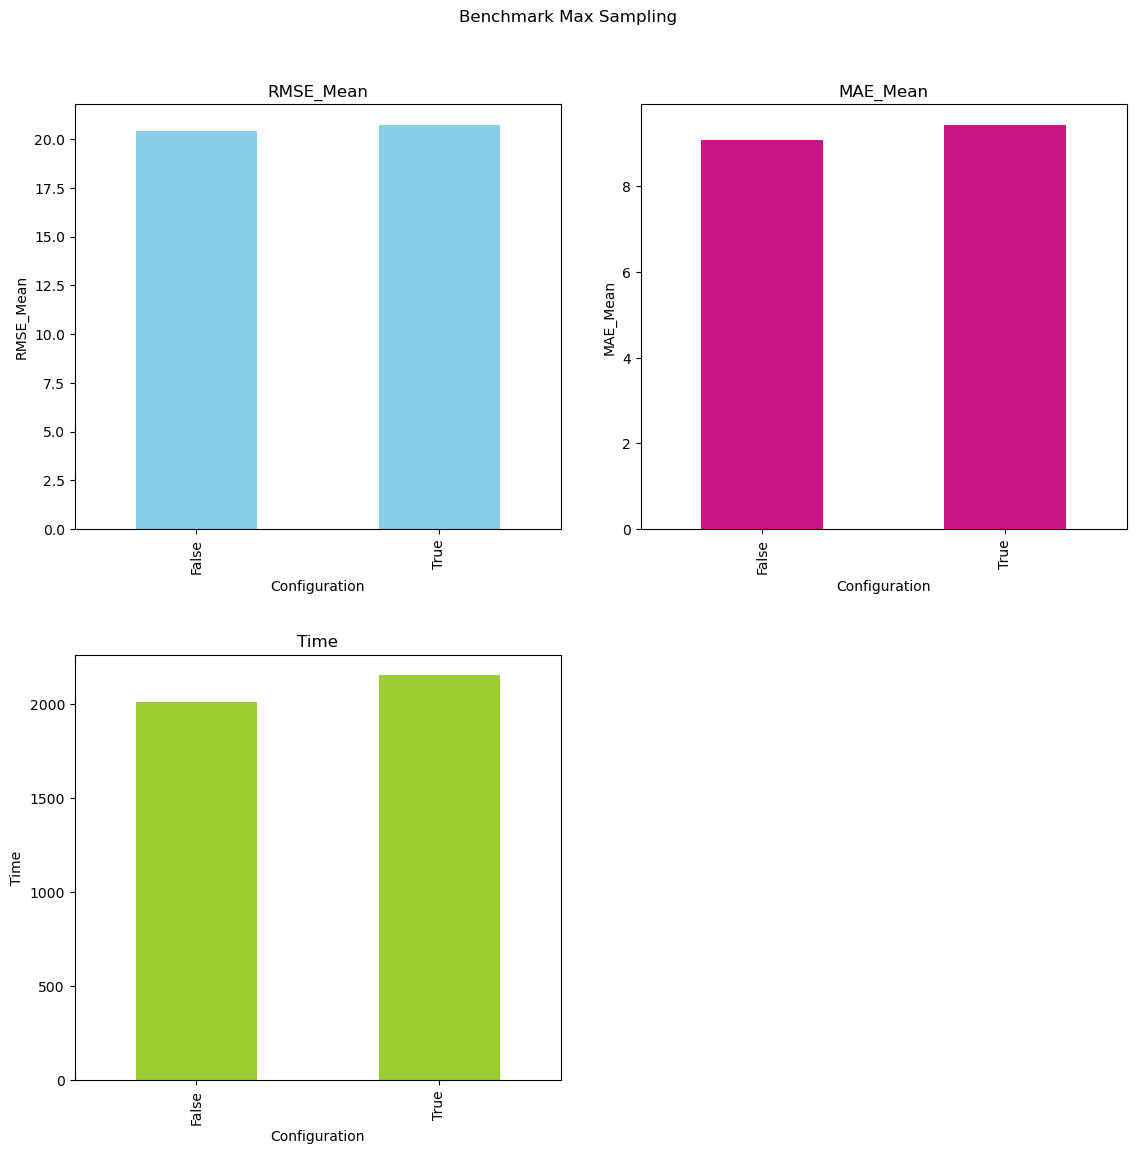
\includegraphics[width=0.8\textwidth]{figures/basic_mh/benchmark/max_sampling.png}
    \captionsetup{width=.8\textwidth}
    \caption{Comparison of the accuracy and the efficiency of Metropolis Hastings algorithms based on the implementation of probability acceptance rate calculation}
    \label{fig:enter-label}
\end{figure}



\subsection{Burn In Phase}
Another crucial part of all Markov chain Monte Carlo algorithms is the discard of the burn-in phase. For Metropolis-Hastings, it is no exception. Determining a general optimal burn in phase leads to an optimization of the result since it is the process of removing generated samples that do not follow the stationary distribution and are unstable. The algorithm was previously executed with a burn-in phase of 20 percent, which means that the first twenty percent of the generated sample data are discarded. However, a comparison to other values of the burn-in phase would give us an overview of how effective the 20 percent is and whether it is enough. The values that are used to compare are $33$ and $50$ percent. On the graph, the values $2$, $3$, and $5$ denote the denominator of the burn in phase, as they should be interpreted as $\frac 1 2$, $\frac 1 3$ and $\frac 1 5$.

Graph 4.14 infers that the case $50$ percent and the case $20$ percent show relatively similar accuracy and efficiency. However, because removing half of the samples might be a bit too much and the similarity in performance, $20$ percent is a better choice. Therefore, for the rest of the execution phase, we keep discarding the first $20$ percent of the samples as the burn-in phase.

\begin{figure}
    \centering
    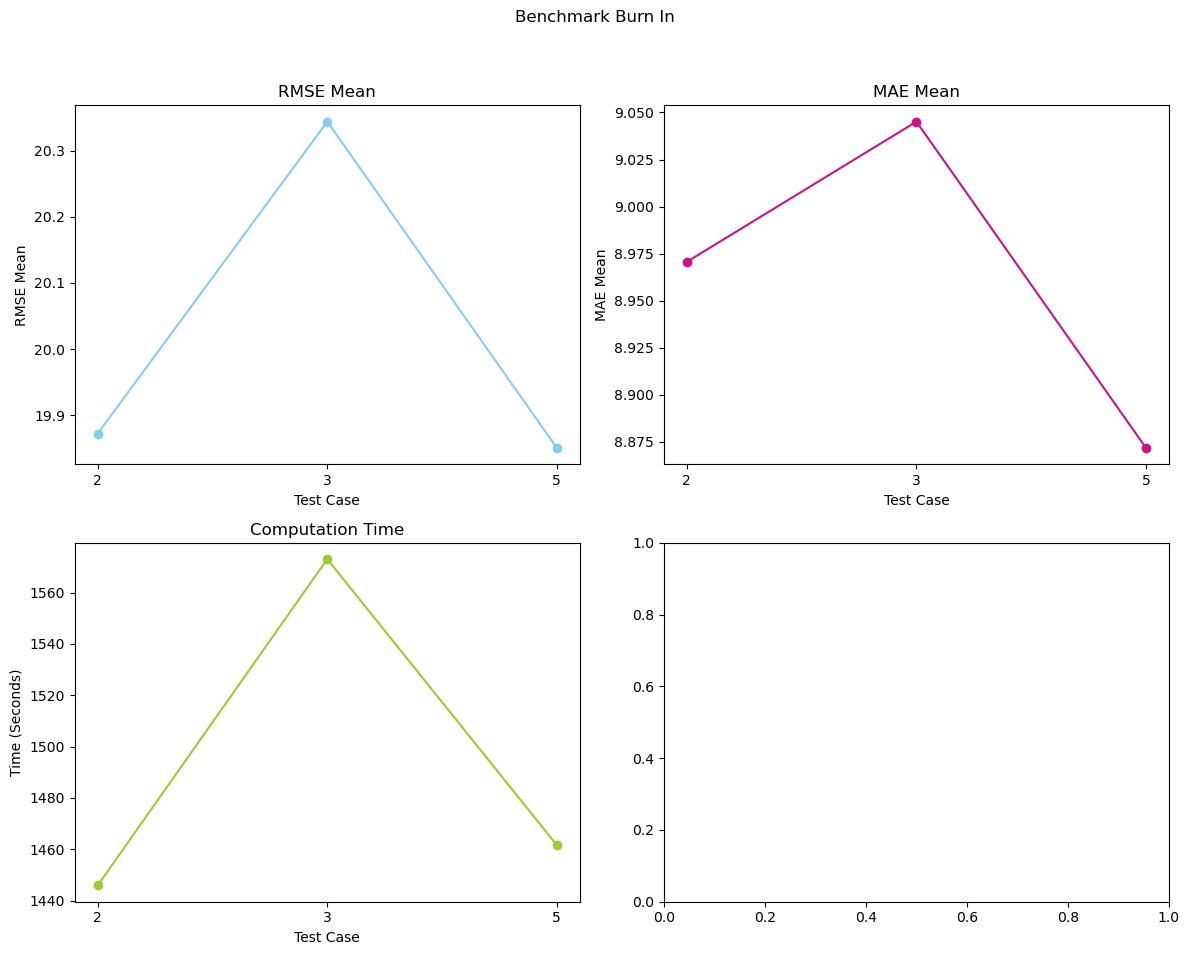
\includegraphics[width=0.8\textwidth]{figures/basic_mh/benchmark/burnin_factor.png}
    \captionsetup{width=.8\textwidth}
    \caption{Comparison of the accuracy and the efficiency of Metropolis Hastings algorithms based on length of burn in phase}
    \label{fig:enter-label}
\end{figure}

\subsection{Effective Sampling Size}
Effective sampling size is a new concept that has not been introduced in this paper until here. It generally measures the number of independent samples equivalent to the correlated samples obtained from the sampling process, which means that it provides us with the number of samples that are independent of each other.\cite{effective_samples_size} The most basic way to implement an effective sampling size in the Markov chain Monte Carlo algorithms is to skip a couple of samples and only regard every several samples in our sample space. The reason to do this is that in Markov chain Monte Carlo algorithms, every sample is dependent on the last sample generated. However, this dependency might have a higher degree of influence, for instance: the newly generated sample is most likely to lie inside of a certain range depending on the standard deviation. Therefore, not considering the sample directly after another might lead to a certain level of independence, which gives rise to more generalization of the sampling space. 

For testing purposes, we compare the algorithm that does not include the effective sampling size feature with algorithms that only consider every second, third, fourth, and fifth sample for the sampling space. The result is shown in Figure 4.15. The efficiency is proportional to the value set for the effective sample size, whereas no pattern could be found for the accuracy aspect. Even though only considering the third sample is relatively less efficient than considering every second sample or even not implementing this feature, it provides better accuracy than all the other cases and relatively better stability due to the low RMSE and MAE of the maximum time series. Therefore, it would be wise for us to keep retaining only the third value from the sample space in the later execution of the Metropolis-Hastings algorithm.

\begin{figure}
    \centering
    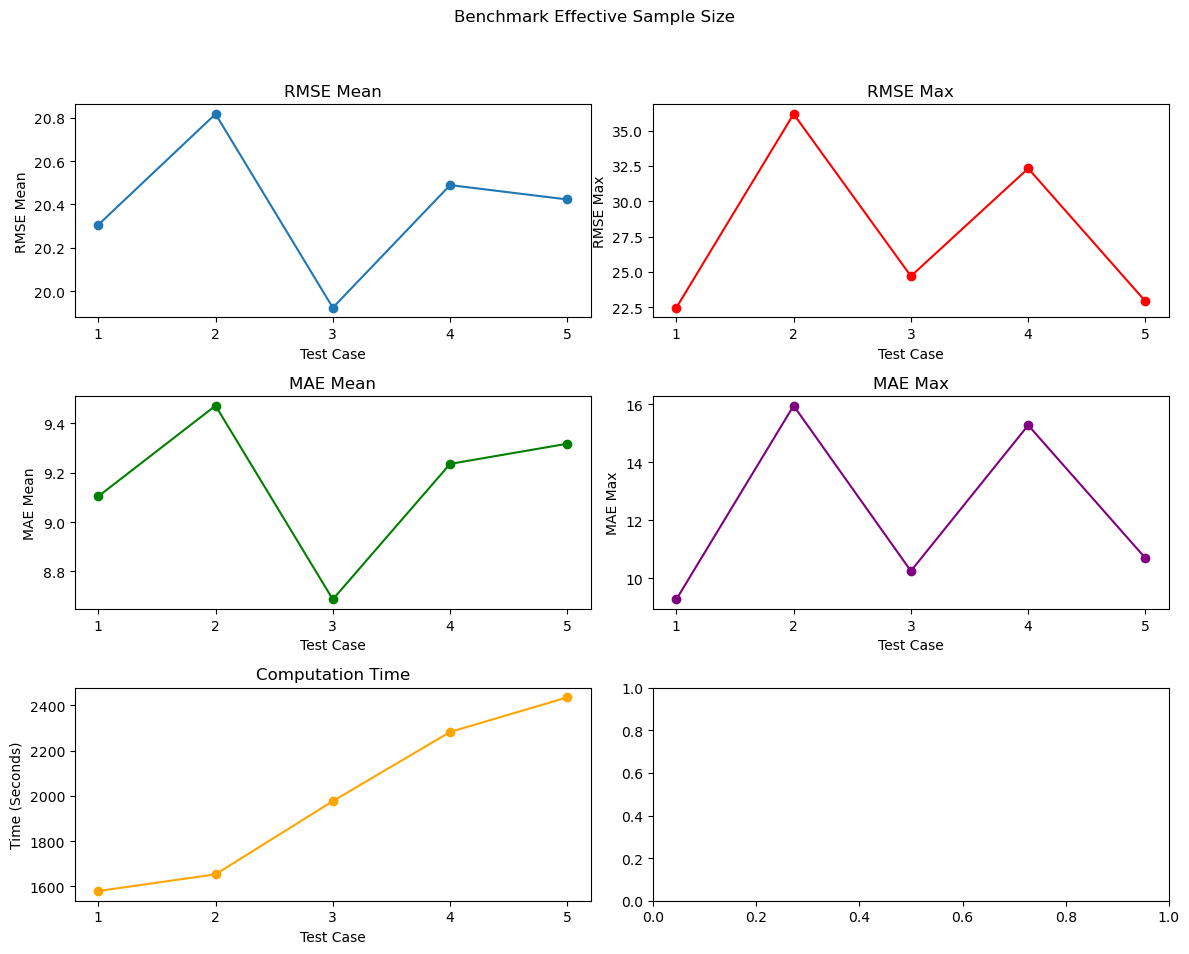
\includegraphics[width=0.8\textwidth]{figures/basic_mh/benchmark/effective_sample_size.png}
    \captionsetup{width=.8\textwidth}
    \caption{Comparison of the accuracy and the efficiency of Metropolis Hastings algorithms based on the selection of effective sample size}
    \label{fig:enter-label}
\end{figure}


\section{Iteration}
Another crucial part of the Metropolis-Hastings algorithm is the amount of iterations. More iterations mean that we can gather more samples. To understand whether the amount of samples that are gathered is enough or not, comparing the accuracy with other numbers of iterations is needed. Until now, we performed the Metropolis-Hastings algorithm with $10000$ iterations. Now we compare this number to other iterations like $5000$, $20000$, $40000$, and $80000$ to find out which number of iterations would deliver the best result and give a decent efficiency.

The result is shown in Figure 4.16, where it is clear to observe that the computation time grows proportionally to the number of iterations. The case of $5000$ delivers the best accuracy and efficiency but might lead to too small of a sample space due to the removal of the burn in period and effective sample size. Of all of the rest cases, they share a similar range of accuracy. However, due to the efficiency of run time, more than $10000$ iterations will be an overkill. Therefore, we continue to execute the algorithm with $10000$ iterations. 

\begin{figure}
    \centering
    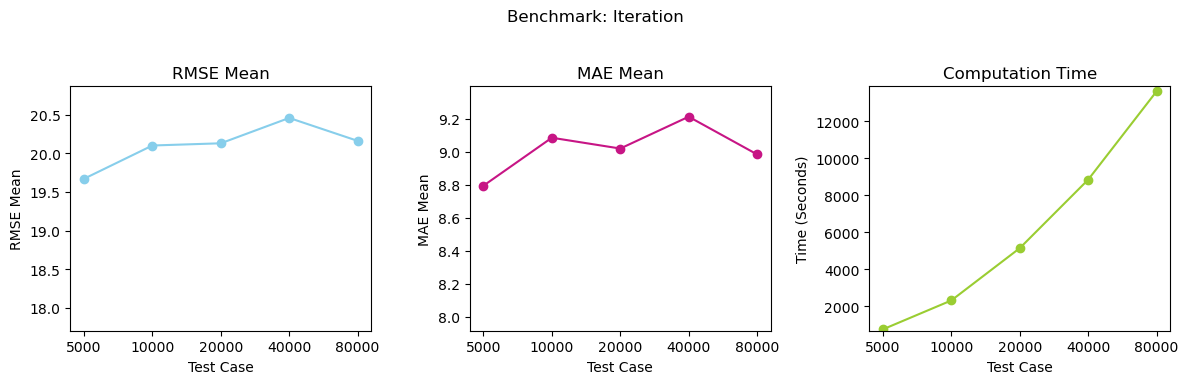
\includegraphics[width=0.8\textwidth]{figures/basic_mh/benchmark/iteration.png}
    \captionsetup{width=.8\textwidth}
    \caption{Comparison of the accuracy and the efficiency of Metropolis Hastings algorithms based on the number of iterations}
    \label{fig:enter-label}
\end{figure}


\subsection{Initial States}
The last input parameter that needs to be explored is the initial states. The initial states should not have that much of an effect on the accuracy, but rather a great influence on the efficiency.\cite{mcmc_practice} A better initial state would allow the algorithm to get rid of the burn-in phase and sample from the stationary distribution sooner, which reduces calculation burdens. It also allows the sampling kernel to discover more samples from the optimal ranges.

Several possible initial states should be taken into consideration. The most general one is the random initial state, used when there is little information regarding the distribution available. To do this, we sample a random state from the posterior and start from here. For testing purposes, however, we randomize 1000 samples and take the mean of them to maximize generalization and randomization. The lower and the upper boundary as the initial values would also work, which requires no initialization at all. Other possible values are derived from prior and posterior distributions. We try the first quantile, the mean, and the third quantile of the prior so that we can figure out whether an optimal starting value is coincidentally near these points. However, the focus point should be on the following three initial states: the first and the third quantile of the posterior distribution as well as the median of the posterior distribution. In the third section of this chapter, we generate a primary result that provides a general result of the posterior distribution. To start the entire algorithm from an inferred posterior state might result in better entry into the algorithm since the starting states are already proven to be very possible on the stationary distribution. Instead of taking the mean of the posterior, we select the median because it represents the half position of the entire posterior distribution, whereas the mean only represents the middle value. It is expected that the most desirable solution comes from one of the proposals of the posterior.

We execute the model with all these different initial states and receive the results shown in Figure 4.17. The RMSE and MAE of the mean time series over all of the test cases prove that the performance is not influenced by the initial states. However, the efficiencies of the algorithms with different initial states do have a massive difference between them. The maximum initialization performs well, as well as the third quantile of the prior, the third quantile of the posterior, and the median of the posterior. After checking the numerical statistics, the median of the posterior delivers the most efficiency as expected. Therefore, it will be set as the default initial state from now on.

\begin{figure}
    \centering
    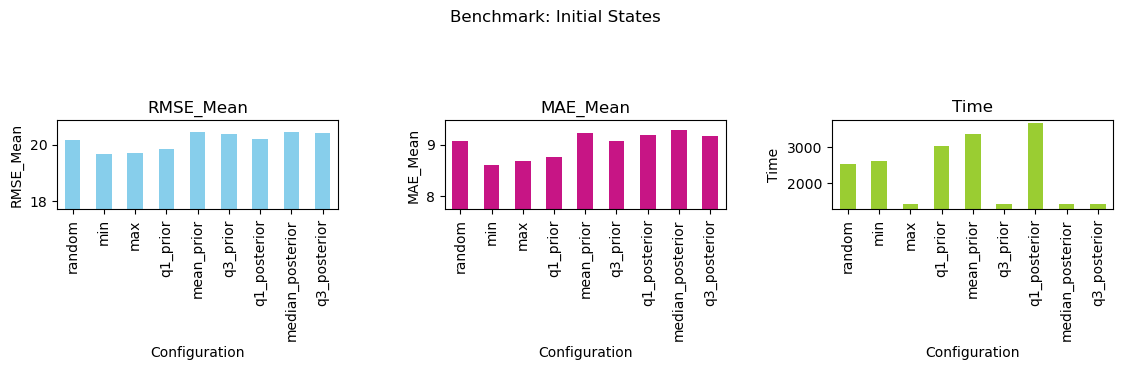
\includegraphics[width=0.8\textwidth]{figures/basic_mh/benchmark/init_method.png}
    \captionsetup{width=.8\textwidth}
    \caption{Comparison of the accuracy and the efficiency of Metropolis Hastings algorithms based on the selection of initial states}
    \label{fig:enter-label}
\end{figure}


\section{Result Comparison}
After evaluating all of the input parameters, we will compare both sets of input parameters by using the Monte Carlo simulation. Using the set of input parameters that deliver the best performance by accuracy metrics in the exploration phase, which will, later on, be called the tuned input parameters, the model will be executed 1000 times, where the RMSE and the MAE of the result time series mean and maximum will be calculated. These results are going to be then compared to those of the models that run on the knowledge-based set of input parameters so that the set of input parameters that delivers better results will be selected to represent the basic Metropolis-Hastings method.

We first draw the histogram and the KDE plot for all of the parameters. It is shown in Figure 4.18. We can observe that the distributions fluctuate more than the parameters from the model that uses the knowledge-based input parameters. In this case, some of the parameters still show irregularity, whereas some of the distributions do show some certain level of resemblance to normal distribution, such as C0, FC, FRAC, and K2. Similar to the case before, the probability of sampling values near both boundaries is relatively low. 

\begin{figure}
    \centering
    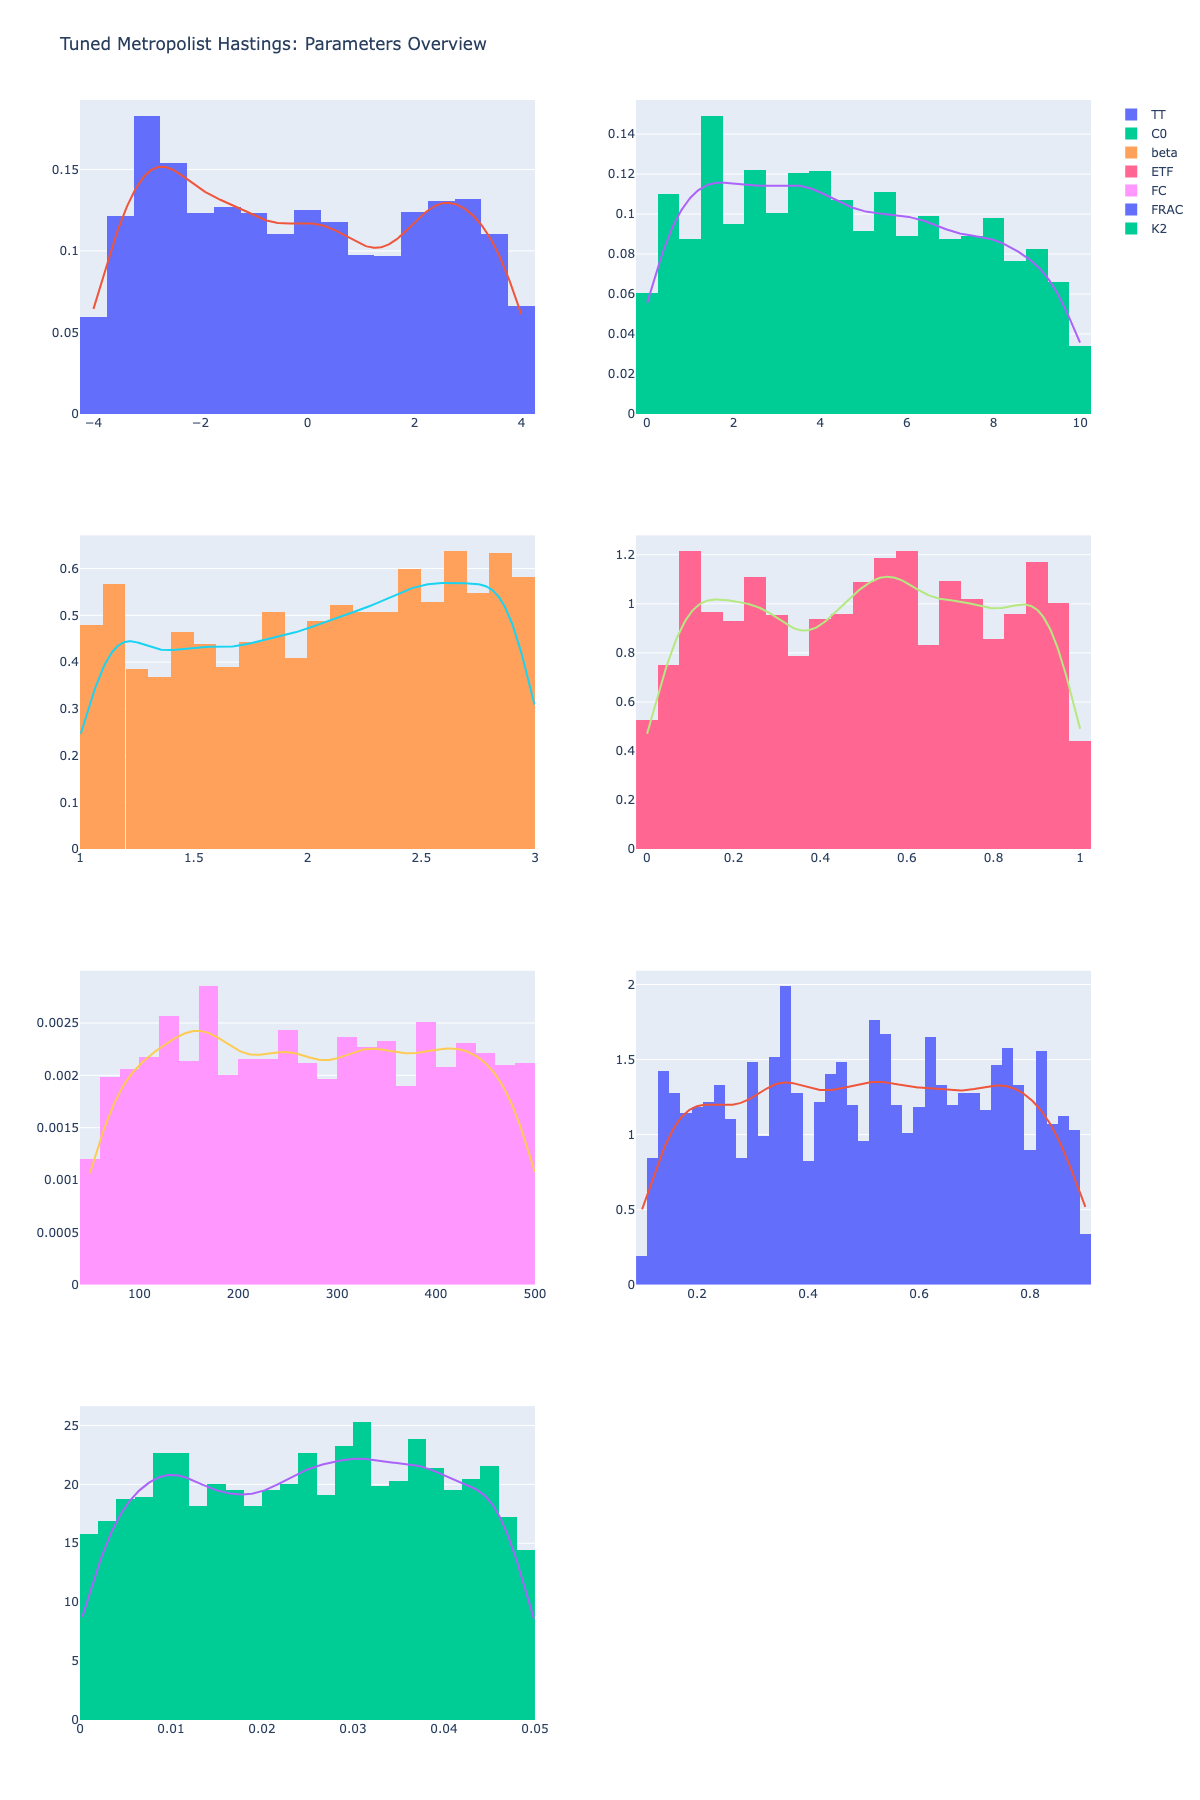
\includegraphics[width=1\textwidth]{figures/basic_mh/tuned_mh/tuned_mh_parameters_overview.png}
    \captionsetup{width=.8\textwidth}
    \caption{Overview of the posterior distribution of the parameters calibrated by the Metropolis Hastings algorithm with tuned input parameters}
    \label{fig:enter-label}
\end{figure}


The boxplots of these parameters are shown in Figure 4.19. We can see that the ranges of most of the sampled parameters are different from the knowledge-based version. The beta and the C0 parameters have moved completely towards the lower bound, whereas the FRAC parameter has moved upwards. The ETF parameter retained its lower bound but had a lower upper bound. In contrast, The TT parameter retained its upper bound, however had a lower bound.


\begin{figure}
    \centering
    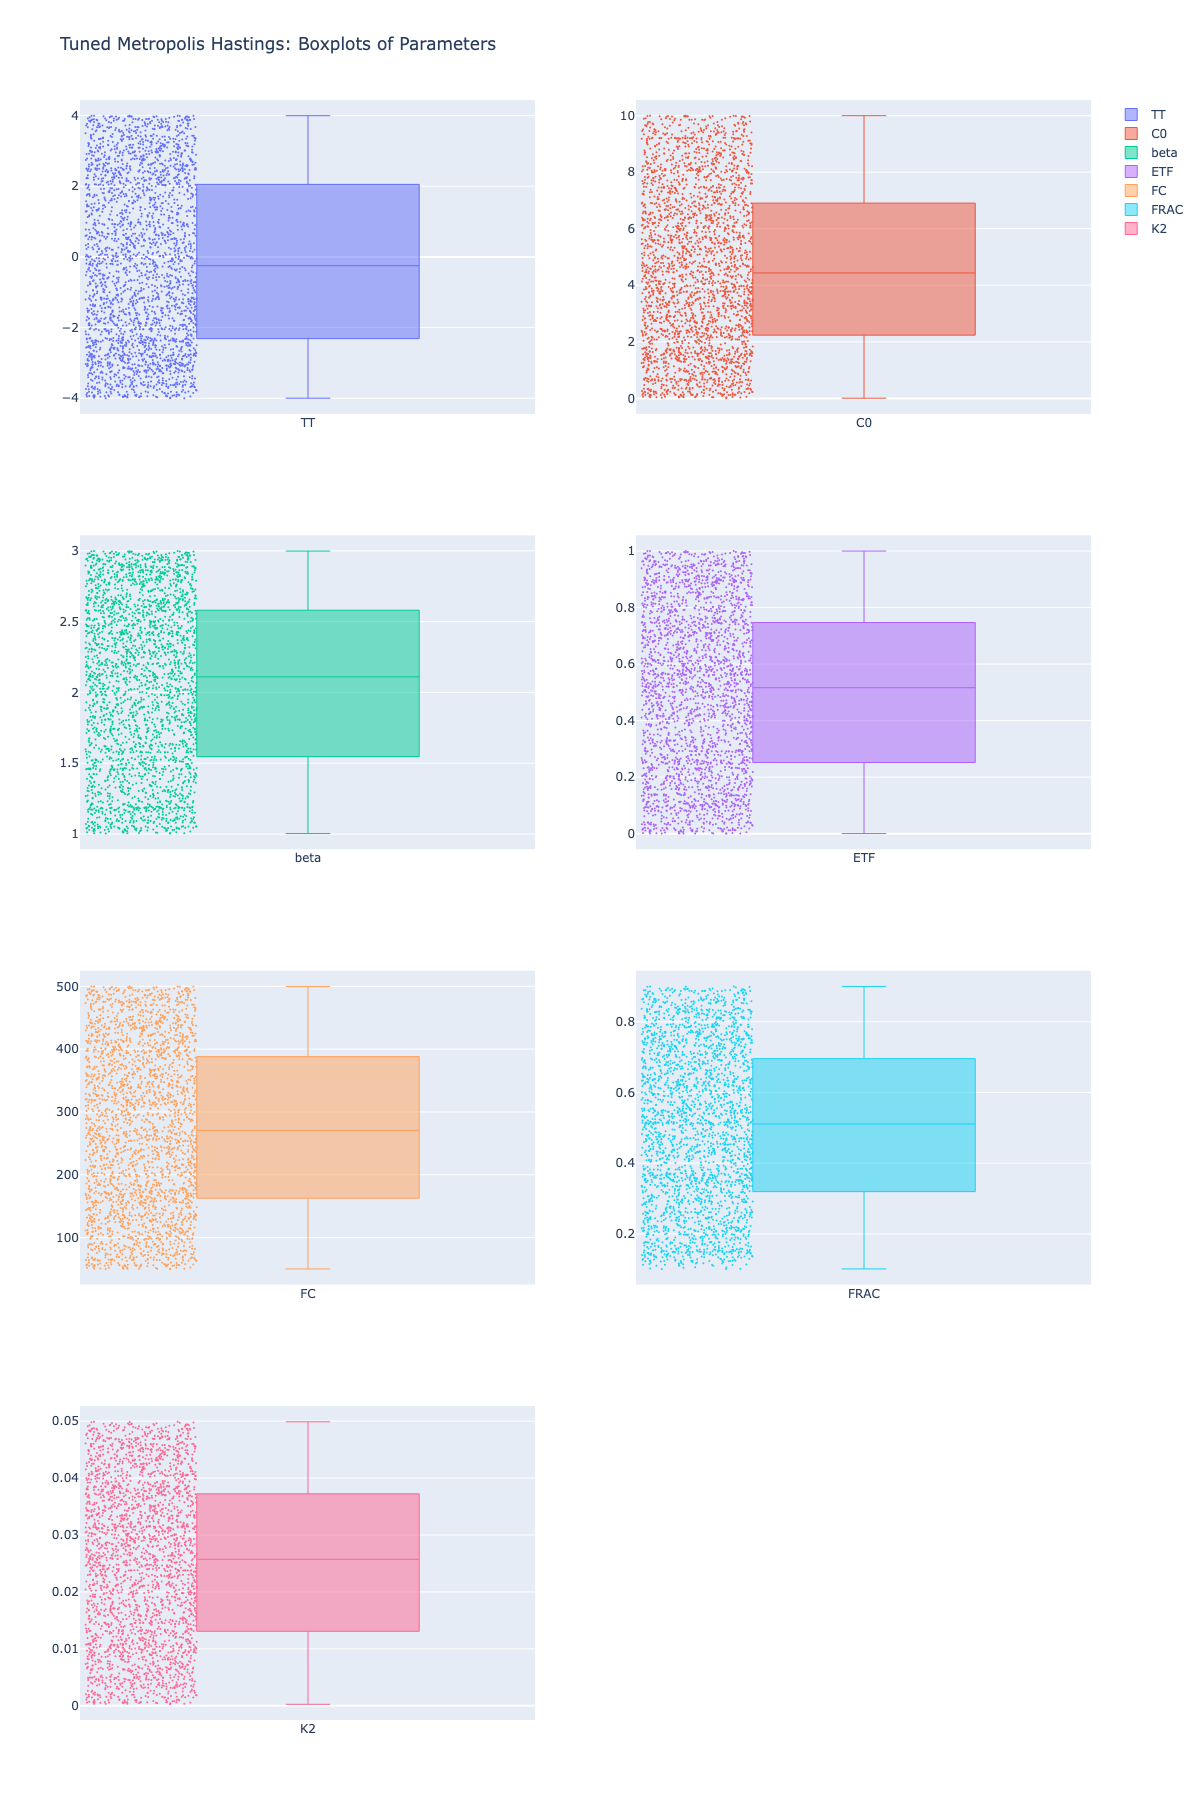
\includegraphics[width=1\textwidth]{figures/basic_mh/tuned_mh/tuned_mh_boxplot.png}
    \captionsetup{width=.8\textwidth}
    \caption{Boxplots of the generated posterior samples of each parameter calibrated by the Metropolis Hastings algorithm with tuned input parameters}
    \label{fig:enter-label}
\end{figure}


The heatmap of the parameter space in Figure 4.20 shows that there are still little to no correlations between each pair of parameters.
\begin{figure}
    \centering
    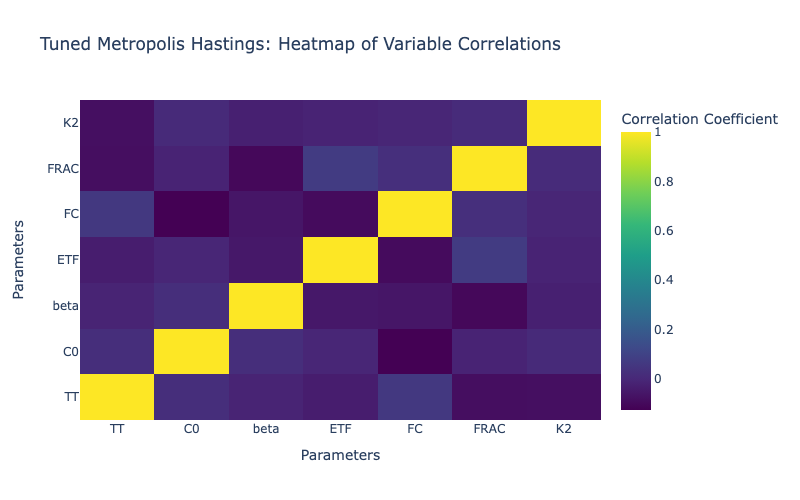
\includegraphics[width=1\textwidth]{figures/basic_mh/tuned_mh/tuned_mh_heatmap.png}
    \captionsetup{width=.8\textwidth}
    \caption{Heatmap between parameters that are calibrated by the Metropolis Hastings algorithm with tuned input parameters}
    \label{fig:enter-label}
\end{figure}

From these generated samples, we retrieve the following result of the Bayesian inference problem shown in Figure 4.21.

\begin{figure}
    \centering
    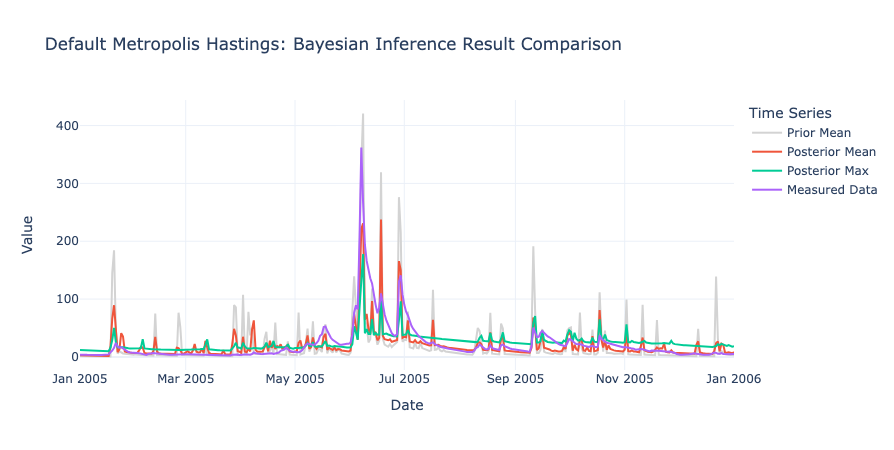
\includegraphics[width=1\textwidth] {figures/basic_mh/tuned_mh/tuned_mh_bayes.png}
    \captionsetup{width=.8\textwidth}
    \caption{Comparison of Bayesian inference results of the Metropolis Hastings with tuned input parameters}
    \label{fig:enter-label}
\end{figure}

To evaluate the result, we keep using the metrics that were calculated before for the model using the knowledged-based set of input parameters, namely RMSE and MAE. The same calculations are executed on the mean and the maximum of the inferred time series. The RMSE of the posterior mean is 21.974609013782757 and the MAE of the posterior mean is 11.457657543376751, whereas the RMSE of the posterior max is 24.458078992931487 and the MAE of the posterior max is 14.532783129590447. The model using the tuned input parameters performs better than the model using the knowledge-based input parameters in some metrics, but not the others. Besides, there is randomness in the Monte Carlo algorithm,\cite{monte_carlo_randomness} which contributes to slightly different values in every single execution.

Therefore, to generalize the accuracy of the result, we run both models 100 times and gather the mean of all the metrics of the results.

\begin{center}
\begin{tabular}{@{}lcc@{}}
\toprule
\textbf{Metric} & \textbf{Knowledge-Based Posterior Mean} & \textbf{Tuned Posterior Mean} \\ \midrule
RMSE            & 22.122504129857315               & 22.124942509212538                  \\
MAE             & 11.400067417022779               & 11.600318945622558              \\ \bottomrule
\end{tabular}
\end{center}




From this table, the knowledge-based input parameters achieve an all-around better performance, but not by much. While the RMSE does not differ from each other that much, the knowledge-based input parameters provide a slightly lower MAE. This might be the case that the inferred time series run by the model using the tuned input parameters performs slightly poorer in predicting extreme data points.

Therefore, we select the knowledge-based input parameters as the default input parameters for the Metropolis-Hastings algorithm for further usage in this paper.




\chapter{Parallel Metropolis Hastings}
In the chapter above, the fundamental Metropolis-Hastings were implemented and evaluated. In this chapter, we modify the fundamental Metropolis-Hastings algorithm, so that it can be run in a parallel way to optimize the run time.

\section{General Idea of Parallel Metropolis Hastings}
In fundamental Metropolis-Hastings, we use a Markov chain to generate new samples. However, it would be possible to fully exploit the parallel computing property and run the algorithm with multiple Markov chains. The general idea would be to use multiple Markov chains instead of one single chain to generate samples. For instance, instead of drawing 10000 samples from one single Markov chain, we draw 2000 samples from each of the five Markov chains simultaneously. 

This modification leads to several aspects that should be discussed. For one, the combination of all of the samples could give rise to some problems. Since the Markov chain will eventually generate a sample from a given stationary distribution, all the samples generated across different chains will be sampled from the same stationary distribution. Therefore, we can simply combine the results after the burn-in period that are derived from different chains. Nevertheless, we need to make sure that all the samples that are generated from the chain after the burn-in period need to be sampled from the stationary distribution. Since each Markov chain from the parallel Metropolis-Hastings generates fewer samples than the amounts of samples that are generated by the Markov chain in the fundamental algorithm, it might be the case that some of the Markov chains do not reach the point where they sample from the stationary distribution. To examine this, we can use the trace plot.\cite{mcmc_practice} It will be discussed in the section "Trace Plot" in this chapter.

Another problem would be the convergence of each dimension. After obtaining the final results, we need to make sure that each dimension of the Bayesian inferred result needs to deliver a converged result, which means that the entire result after the combination is stable and representative and reaches a stationary distribution. In a later section called "Gelman Rubin Convergence", we use the metric of Gelman Rubin Convergence to examine whether the Bayesian inferred result for the hydrological model using the parallel Metropolis-Hastings reaches convergence.

\section{Efficiency Analysis}
Since the machine, on which the algorithm is run, has 10 cores of CPUs, we are going to experiment with this algorithm with 10, 8, 5, 4, and 2 chains. These cases will be compared with the fundamental Metropolis-Hastings algorithm, where only one single chain is run. To analyze the algorithm concerning its efficiency, we record the run time of the algorithm using different numbers of chains. The result is represented in the figure 5.1. It is obvious to see that the run time and the number of chains display an inverse proportional relationship. The more chains that are used, the less time is required for the algorithm to run, and vice versa.

\begin{figure}[H]
    \centering
    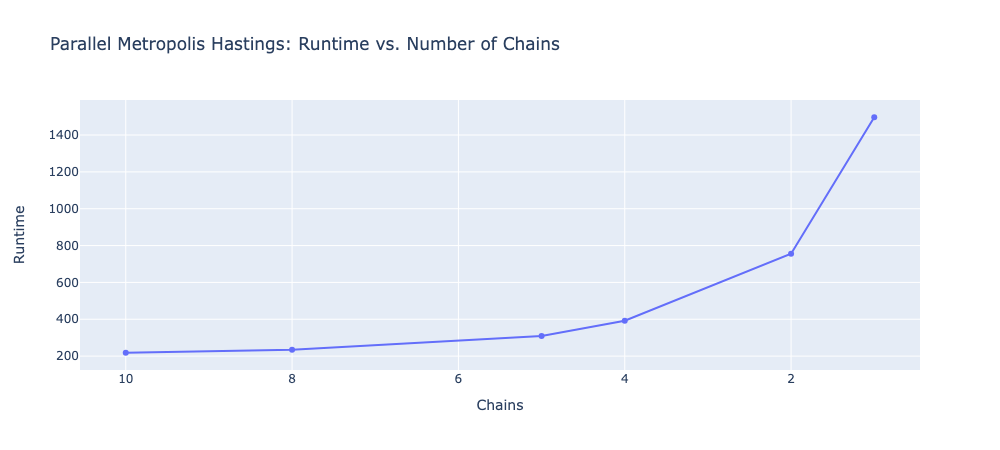
\includegraphics[width=1\textwidth]{figures/parallel_mh/runtime.png}
    \captionsetup{width=.8\textwidth}
    \caption{Relationship between run time and chain numbers for parallel Metropolis Hastings algorithm}
    \label{fig:enter-label}
\end{figure}

\section{Trace Plot}
Making sure that each Markov chain generates samples from the stationary distribution is crucial in the parallel Metropolis-Hastings algorithm. The best way to examine this aspect is to visualize the trace of each sample generated from the chain.\cite{mcmc_practice} The trace plot tracks each sample generated by the algorithm and plots the position of each sample by order. In this case, we can observe which sample is generated based on the last sample.

As mentioned before, it is more likely that the parallel Metropolis-Hastings algorithm with more chains shows less probability of sampling from stationary distribution than the parallel Metropolis-Hastings algorithm with fewer chains. This aspect is going to be analyzed now. We first select random chains from the algorithm run with the most number of chains, namely $10$, and the least number of chains, which is $2$, to observe the two extreme cases. Since 1000 samples are generated by each chain from the case of $10$ chains, only $266$ samples are going to be recorded after discarding $20\%$ of the burn-in and using $3$ as the effective sample size. With the case of $2$ chains, the number of samples recorded has risen to $1333$, which is almost $5$ times as much as the previous case. This shows a higher probability that the samples are generated from the stationary distribution.

For both cases, two chains are selected for visualization to ensure the generality of the analysis. The figures of the trace plots are displayed in Figures 5.2 to 5.5. One major difference between the visualizations of both cases is that the chain for case $10$ includes more abrupt jumps throughout the entire sampling process, whereas abrupt jumps occur less after the starting period is over for case $2$. The longer chain in the case of $2$ generally provides better stability and convergence of the parameter estimates. With no obvious sampling trends and full exploration of the entire parameter space, it is observable that every parameter for the chain has settled into a stationary distribution that covers the entire parameter space. The shorter chain in the case of $10$ may not enter the convergence and can be more susceptible to initial conditions or random fluctuations. Therefore, observing the trace plot for each chain after executing the algorithm is important, especially for algorithms that are run with more chains, each of which generates fewer samples.

\begin{figure}[H]
    \centering
    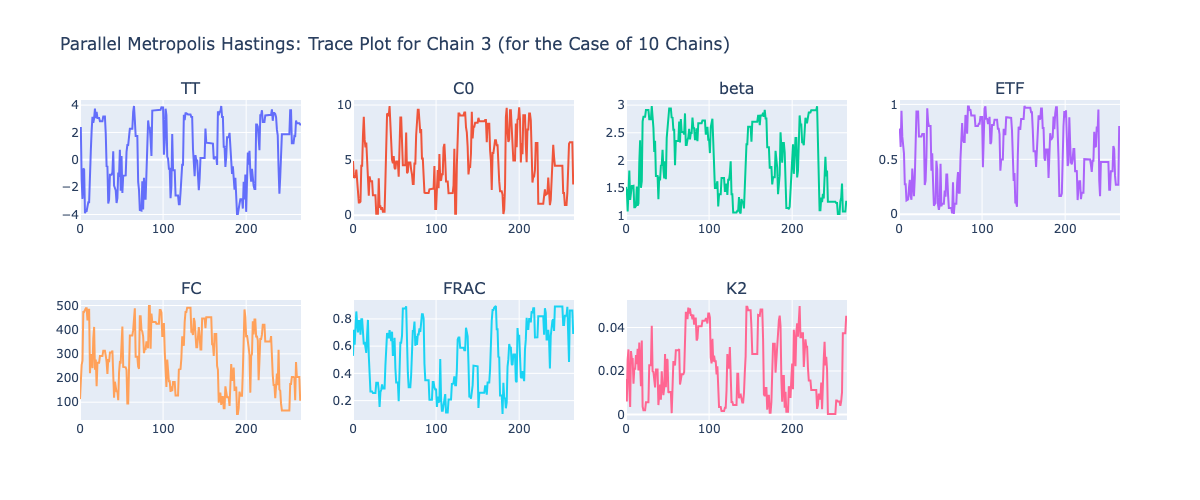
\includegraphics[width=1\textwidth]{figures/parallel_mh/tp_rand_10_3.png}
    \captionsetup{width=.8\textwidth}
    \caption{Trace plot of the third chain from the parallel Metropolis Hastings algorithm with 10 chains}
    \label{fig:enter-label}
\end{figure}

\begin{figure}[H]
    \centering
    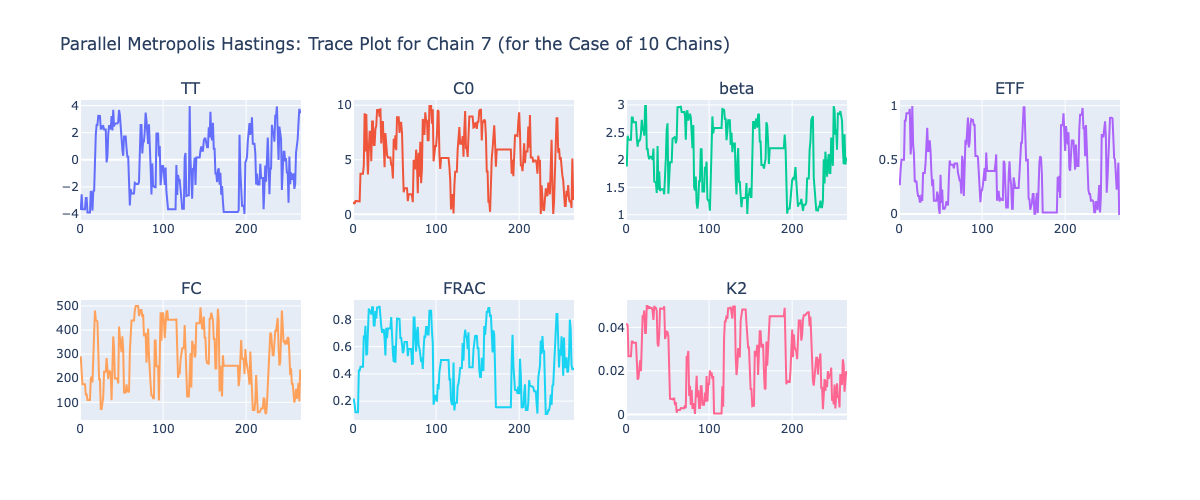
\includegraphics[width=1\textwidth]{figures/parallel_mh/tp_rand_10_7.png}
    \captionsetup{width=.8\textwidth}
    \caption{Trace plot of the seventh chain from the parallel Metropolis Hastings algorithm with 10 chains}
    \label{fig:enter-label}
\end{figure}

\begin{figure}[H]
    \centering
    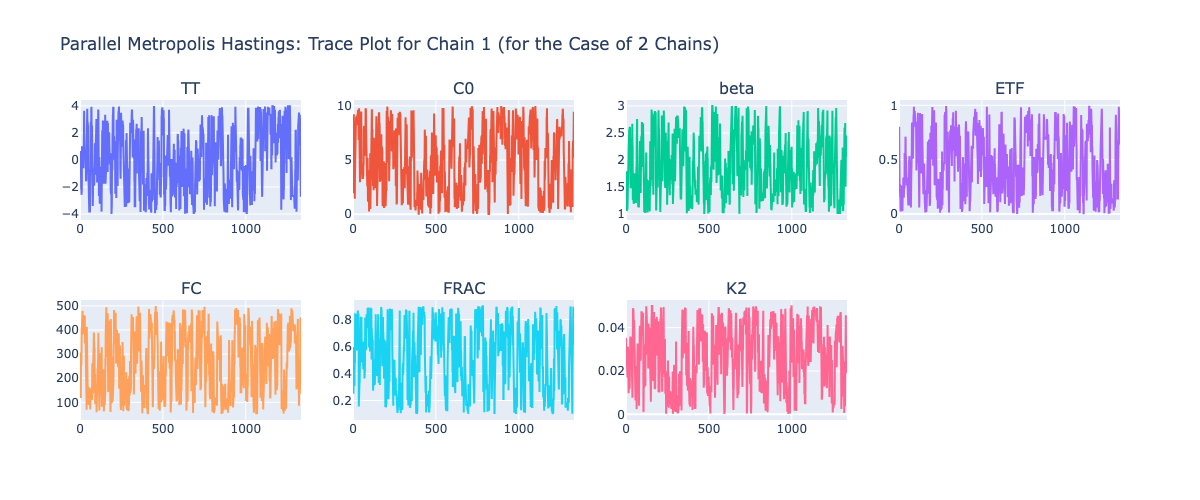
\includegraphics[width=1\textwidth]{figures/parallel_mh/tp_rand_2_1.png}
    \captionsetup{width=.8\textwidth}
    \caption{Trace plot of the first chain from the parallel Metropolis Hastings algorithm with 2 chains}
    \label{fig:enter-label}
\end{figure}

\begin{figure}[H]
    \centering
    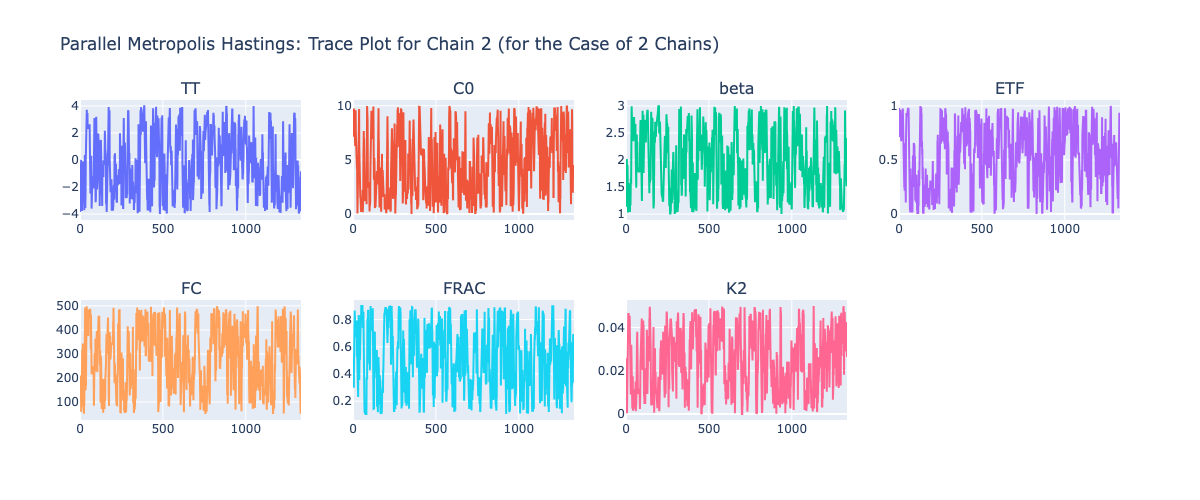
\includegraphics[width=1\textwidth]{figures/parallel_mh/tp_rand_2_2.png}
    \captionsetup{width=.8\textwidth}
    \caption{Trace plot of the second chain from the parallel Metropolis Hastings algorithm with 2 chains}
    \label{fig:enter-label}
\end{figure}


\section{Gelman Rubin Convergence}
As we mentioned in the introduction of this chapter, the convergence of the result is an aspect that we shall observe after combining all results altogether. This diagnostic helps to determine whether the chains have reached a stationary distribution over time, which shows whether the samples are representative of the target distribution.\cite{gelman_rubin}

The calculation of Gelman Rubin's diagnostic looks as follows: We define $m$ as the number of chains and $n$ as the number of iterations of each chain. $s_{ij}$ is then the vector of parameters in the $i$th iteration of from the $j$th chain. $\overline{s}_j$ is the mean of vectors within the $j$th chain, whereas $\overline{s}$ is the grand mean vector, calculating the mean of all of the $\overline{s}_j$.\cite{gr_calc}

\begin{align}
W = \frac 1 {m(n-1)}\sum_{j=1}^m \sum_{i=1}^n (s_{ij} - \overline{s}_j)^2
\end{align}

\begin{align}
B = \frac n {m-1} \sum_{j=1}^m (\overline{s}_j - \overline{s})^2
\end{align}

\begin{align}
V = \frac {n-1}n W + (1 + \frac 1 m)\frac B n
\end{align}

\begin{align}
R = \frac V W
\end{align}

$W$ is called the within-chain variance estimates, which estimate the variances of all sampled points within chains. $B$ is called the average of the between, which measures the variance of the chain means around the overall mean of these means. $V$ is the pooled variance estimate, which is calculated by the weighted versions of $B$ and $W$. Last but not least, the ratio between the pooled an d within chain estimators is calculated and used as the Gelman-Rubin diagnostic. If the diagnostic is close to 1, commonly less than 1.1, it suggests that the chains have converged to the target distribution. A value greater than 1.1 indicates that additional sampling may be necessary, or that the chains have not yet mixed well and may potentially need more iterations.\cite{gr_calc} For the case of MCMC, the threshold of 1.2 is also tolerated.\cite{gr1.2}

We now take a look at the performance of Gelman Rubin's convergence in the parallel Metropolis-Hastings algorithm. We take a look at the algorithms with different chain numbers, They are displayed in Figures 5.6 to 5.10. All of these cases show a good enough convergence to show compliance to the threshold of $1.1$, even though a relationship between the convergence level and the number of chains could be found: the more chains there are, the less the result converges.

The reason behind this observation is that each chain generates fewer samples if more chains are used in the parallel Metropolis-Hastings algorithm. In this case, it is more likely that individual chains reach a low level of convergence since it does not generate enough samples. For instance, even though it still satisfies the convergence threshold, the case of $10$ chains shows the worst convergence level of all of the test cases, since it only generates $1000$ samples instead of $2500$ in the case of $4$ chains. Another observation is that no patterns can be found regarding the convergence behavior of individual dimensions. No parameter performs the best or the worst in every single case, which means that further investigation of individual parameters is not needed.

\begin{figure}[H]
    \centering
    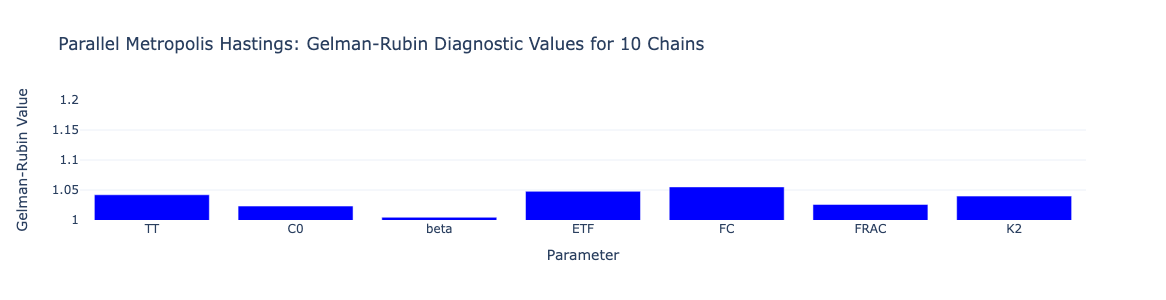
\includegraphics[width=1\textwidth]{figures/parallel_mh/GR_10.png}
    \captionsetup{width=.8\textwidth}
    \caption{Gelman Rubin Convergence Diagnostic of the parallel Metropolis Hastings algorithm with 10 chains}
    \label{fig:enter-label}
\end{figure}

\begin{figure}[H]
    \centering
    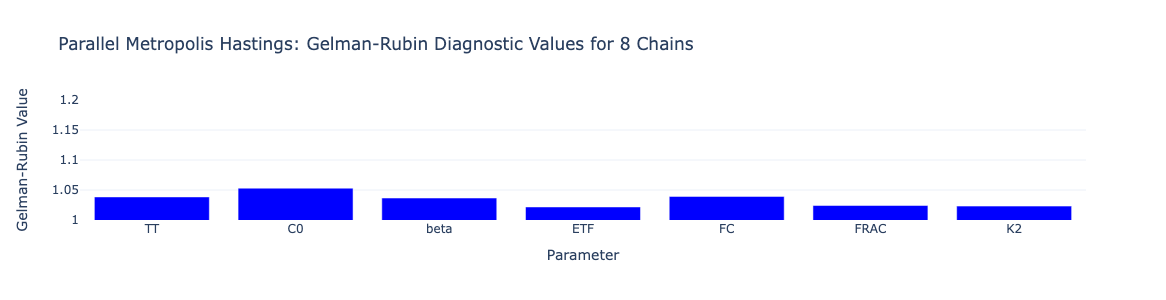
\includegraphics[width=1\textwidth]{figures/parallel_mh/GR_8.png}
    \captionsetup{width=.8\textwidth}
    \caption{Gelman Rubin Convergence Diagnostic of the parallel Metropolis Hastings algorithm with 8 chains}
    \label{fig:enter-label}
\end{figure}

\begin{figure}[H]
    \centering
    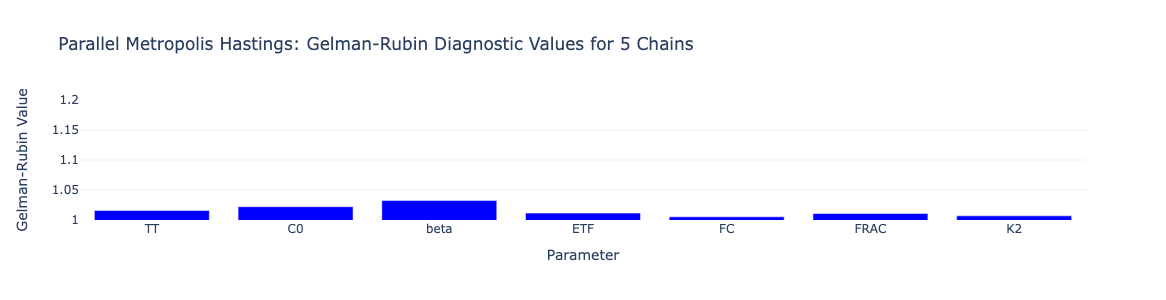
\includegraphics[width=1\textwidth]{figures/parallel_mh/GR_5.png}
    \captionsetup{width=.8\textwidth}
    \caption{Gelman Rubin Convergence Diagnostic of the parallel Metropolis Hastings algorithm with 5 chains}
    \label{fig:enter-label}
\end{figure}

\begin{figure}[H]
    \centering
    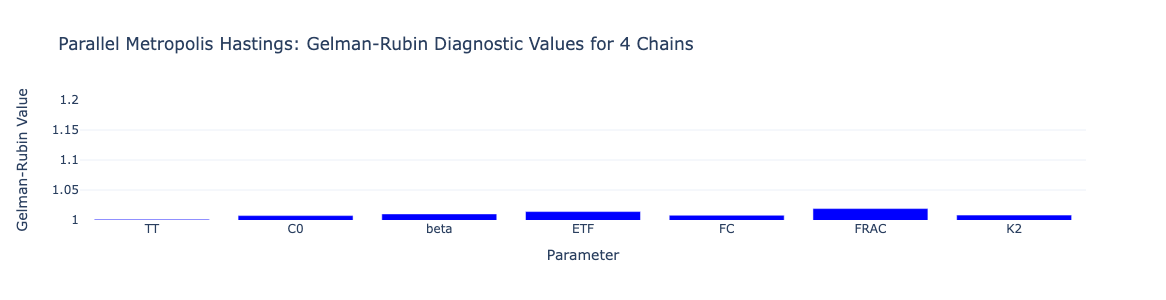
\includegraphics[width=1\textwidth]{figures/parallel_mh/GR_4.png}
    \captionsetup{width=.8\textwidth}
    \caption{Gelman Rubin Convergence Diagnostic of the parallel Metropolis Hastings algorithm with 4 chains}
    \label{fig:enter-label}
\end{figure}

\begin{figure}[H]
    \centering
    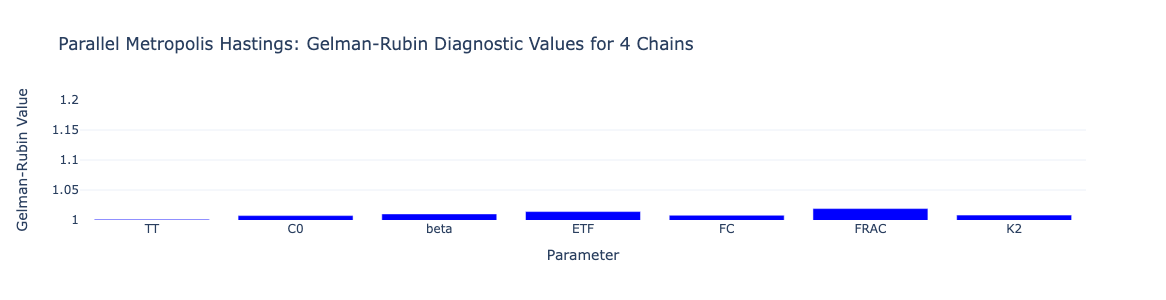
\includegraphics[width=1\textwidth]{figures/parallel_mh/GR_2.png}
    \captionsetup{width=.8\textwidth}
    \caption{Gelman Rubin Convergence Diagnostic of the parallel Metropolis Hastings algorithm with 2 chains}
    \label{fig:enter-label}
\end{figure}



\section{Autocorrelation Plot}
An autocorrelation plot displays the correlation of a series with itself at different levels of lags. In the context of MCMC, it shows the dependency of the current value in the chain and its past values. This plot is crucial because samples that are generated by Markov chain Monte Carlo algorithms are inherently sequential and may exhibit significant correlation with previous samples, which is something that should be investigated. 

In this section, the autocorrelation of each of the Metropolis-Hastings cases regarding the number of chains is investigated. Since we draw the conclusion from the chapter above that the most optimal effective sample size is $3$, we keep using this number in these test cases.

We first take a look at the cases with the most and the least number of chains, namely $10$ and $2$. These can be found in Figures 5.11 and 5.12. Both autocorrelation graphs share a characteristic that the autocorrelation drops to a low level quickly within a few lags. This suggests that the influence of any given sample on future samples diminishes quickly, which indicates good sampling efficiency. Afterwards, for both cases, the autocorrelation of all dimensions oscillates around 0 and 0.2 positive and negative, which suggests that the sampling shows stability and low correlation to past samples. 

\begin{figure}[H]
    \centering
    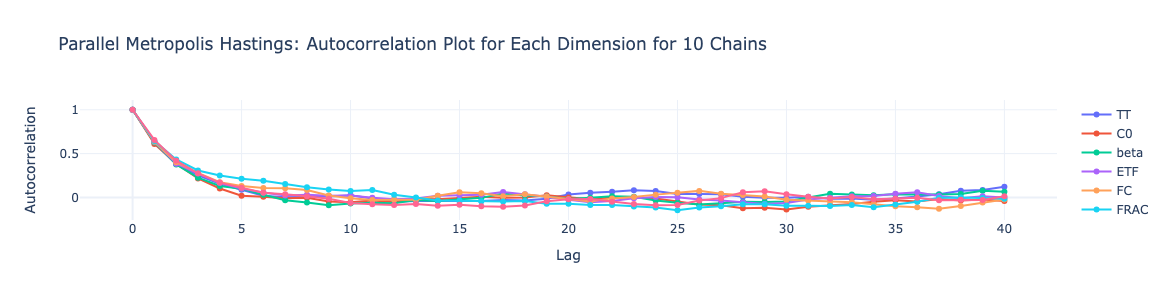
\includegraphics[width=1\textwidth]{figures/parallel_mh/Autocorrelation_10.png}
    \captionsetup{width=.8\textwidth}
    \caption{Autocorrelation plot of the parallel Metropolis Hastings algorithm with 10 chains}
    \label{fig:enter-label}
\end{figure}


\begin{figure}[H]
    \centering
    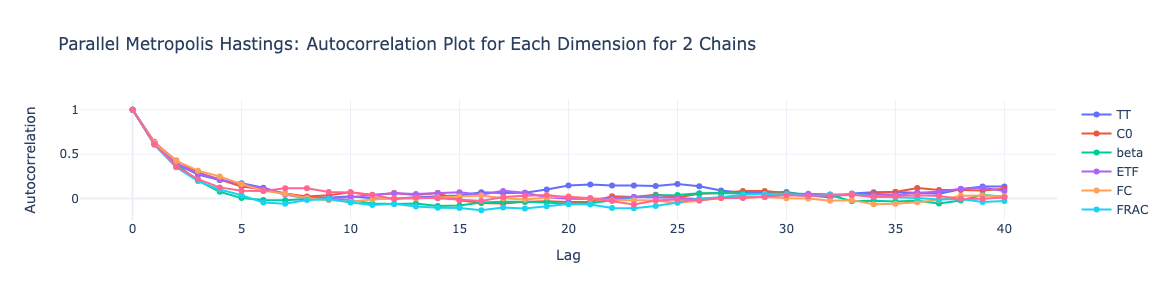
\includegraphics[width=1\textwidth]{figures/parallel_mh/Autocorrelation_2.png}
    \captionsetup{width=.8\textwidth}
    \caption{Autocorrelation plot of the parallel Metropolis Hastings algorithm with 2 chains}
    \label{fig:enter-label}
\end{figure}


However, both graphs do not display an extremely low level of autocorrelation at high lags. For some parameters, the autocorrelation at high lags approaches $0.2$, which is a relatively high value, even though it is generally acceptable. After plotting graphs for more test cases of the parallel Metropolis-Hastings algorithm using different chains, the autocorrelation graph of the parallel Metropolis-Hastings algorithm using 8 chains delivers a more optimal result. This can be seen in Figure 5.13. Autocorrelations around 20 lags approach closer to zero or show minimal fluctuation around zero. However, the autocorrelation around 40 lags shows a closer distance to 0, which is optimal for the independence property of Markov chain sampling. Nevertheless, all of the other cases of chain numbers show a satisfying result, with rapid diminishing in the first few lags, oscillation around zero, and a relatively low level of autocorrelation for all of the lags apart from the first few.


\begin{figure}[H]
    \centering
    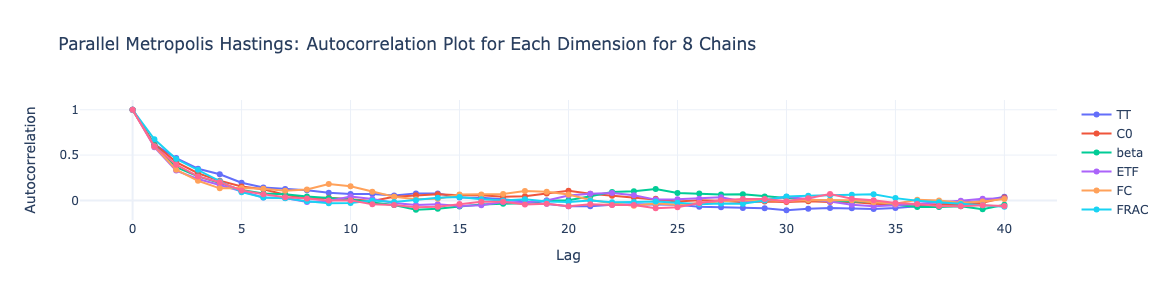
\includegraphics[width=1\textwidth]{figures/parallel_mh/Autocorrelation_8.png}
    \captionsetup{width=.8\textwidth}
    \caption{Autocorrelation plot of the parallel Metropolis Hastings algorithm with 8 chains}
    \label{fig:enter-label}
\end{figure}


\section{Accuracy Analysis by Chains}
After all these analyses regarding the components of the algorithm, we shall determine the number of chains that suit the algorithm the best. The accuracy metrics are kept the same as the ones that are used in the chapters above the RMSE and MAE. From the graphs shown in Figures 5.14 and 5.15, the parallel Metropolis-Hastings algorithm using 4 chains shows the best level of accuracy in both metrics. Centered around 4, the further the number of chains are, the less accurate they are, however not by a significant difference.

\begin{figure}[H]
    \centering
    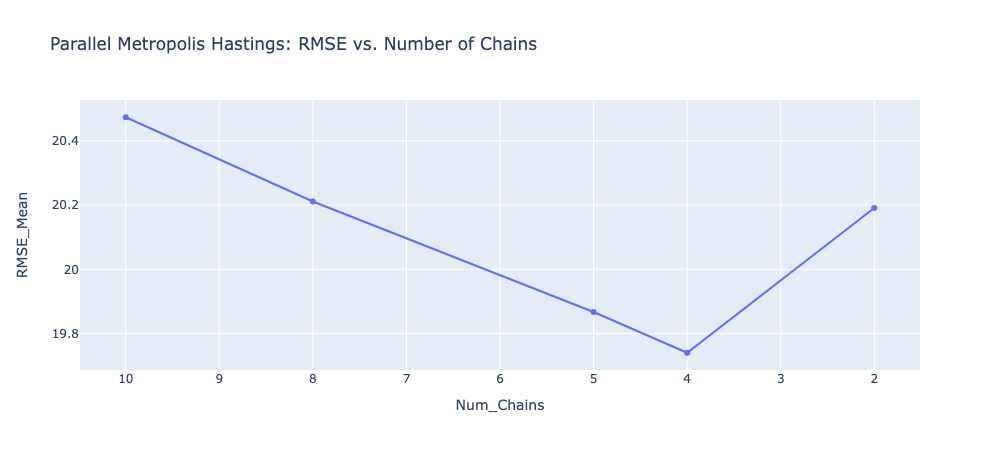
\includegraphics[width=1\textwidth]{figures/parallel_mh/rmse.png}
    \captionsetup{width=.8\textwidth}
    \caption{Mean RMSE of the parallel Metropolis Hastings algorithm across test cases with different chains}
    \label{fig:enter-label}
\end{figure}

\begin{figure}[H]
    \centering
    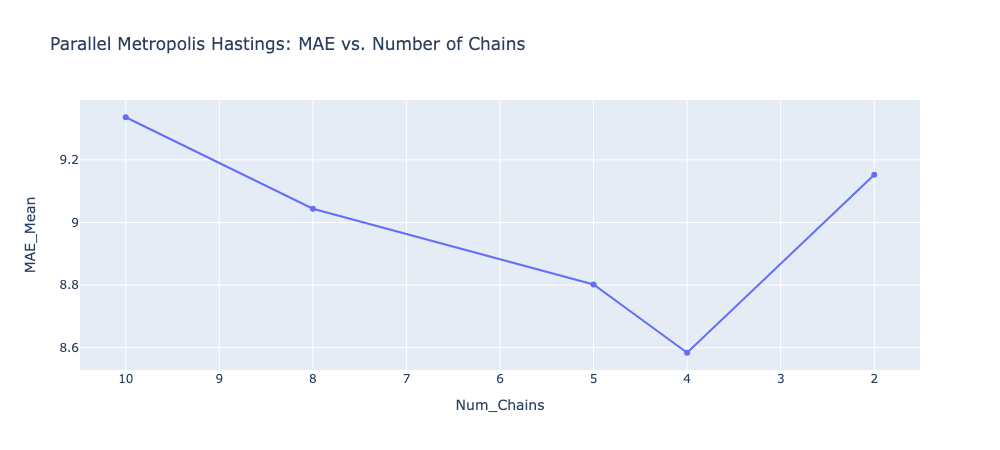
\includegraphics[width=1\textwidth]{figures/parallel_mh/mae.png}
    \captionsetup{width=.8\textwidth}
    \caption{Mean MAE of the parallel Metropolis Hastings algorithm across test cases with different chains}
    \label{fig:enter-label}
\end{figure}

\section{Parameter Overview}
The last aspect that is focused on in this chapter is the inferred parameter. In the chapter above, we visualized the inferred parameter by visualizing the distribution of the individual parameters. For the case of parallel Metropolis-Hastings, we utilize multiple chains to sample. Therefore, it is a good idea for us not only just to visualize the inferred parameter distribution of the entire result, but also to visualize the inferred parameter distribution of each chain and to compare them with the result, to review the stability of the sampling of each chain and also finding out similarities and patterns.

As usual, we first analyze the parameters by a chain for the two extreme cases, namely parallel Metropolis-Hastings with $10$ and with $2$ chains. These can be found in Figures 5.16 and 5.18. From the case of $10$ chains, we can see that the distribution of each chain is relatively random. To compose the distribution of the combined results, each chain is responsible for exploring a different region. For instance, for the parameter TT, the $9$th chain explores the side with lower values more, whereas the $10$th chain is more responsible for the side with higher values. Altogether, this property contributes to the relatively uniform distribution of the combined result. However, there are still similarities to some extent that can be found between the sample distribution of each chain and the sample distribution of the combined result. In each distribution, there are two peaks, each located on the left and the right side of a trough. This means that in each sampling process, two regions can be found that aggregate the most sampling values. Besides, both regions on the left and the right side of the interval acquire fewer samples than other regions, which contribute to the same property of the final combined result. In the case of $2$ chains, things are not so complicated. Because each chain generated more samples than each chain does for the case of $10$ chains, the distribution of each chain looks highly similar to the distribution of the combined result for most of the parameters. For the parameter of ETF, as an exception, it shares the property as the case for $10$ chains, namely that both of the chains are responsible for exploring two different areas, which are the left and the right sides of the entire interval.

Another plot that is used for visualizing the parameters is the boxplot, which is also visualized here in the same way as above: each chain is visualized individually, where they are compared to each other and the combined result boxplot afterward. The figures for cases of $10$ chains and $2$ chains can be found below in Figures 5.17 and 5.19. The results that we can draw from observing these boxplot graphs are the same as the conclusion that we have drawn above for the case of more chains, the $1$st quantile, the median and the $3$ quantile all vary from each other, which means that each chain is responsible for different regions. For the case of fewer chains, however, the $1$st quantile, the median, and the $3$ quantile lie almost on the same level or do not vary from each other that much, indicating that the samples from each chain are more stabilized. 

\begin{figure}[H]
    \centering
    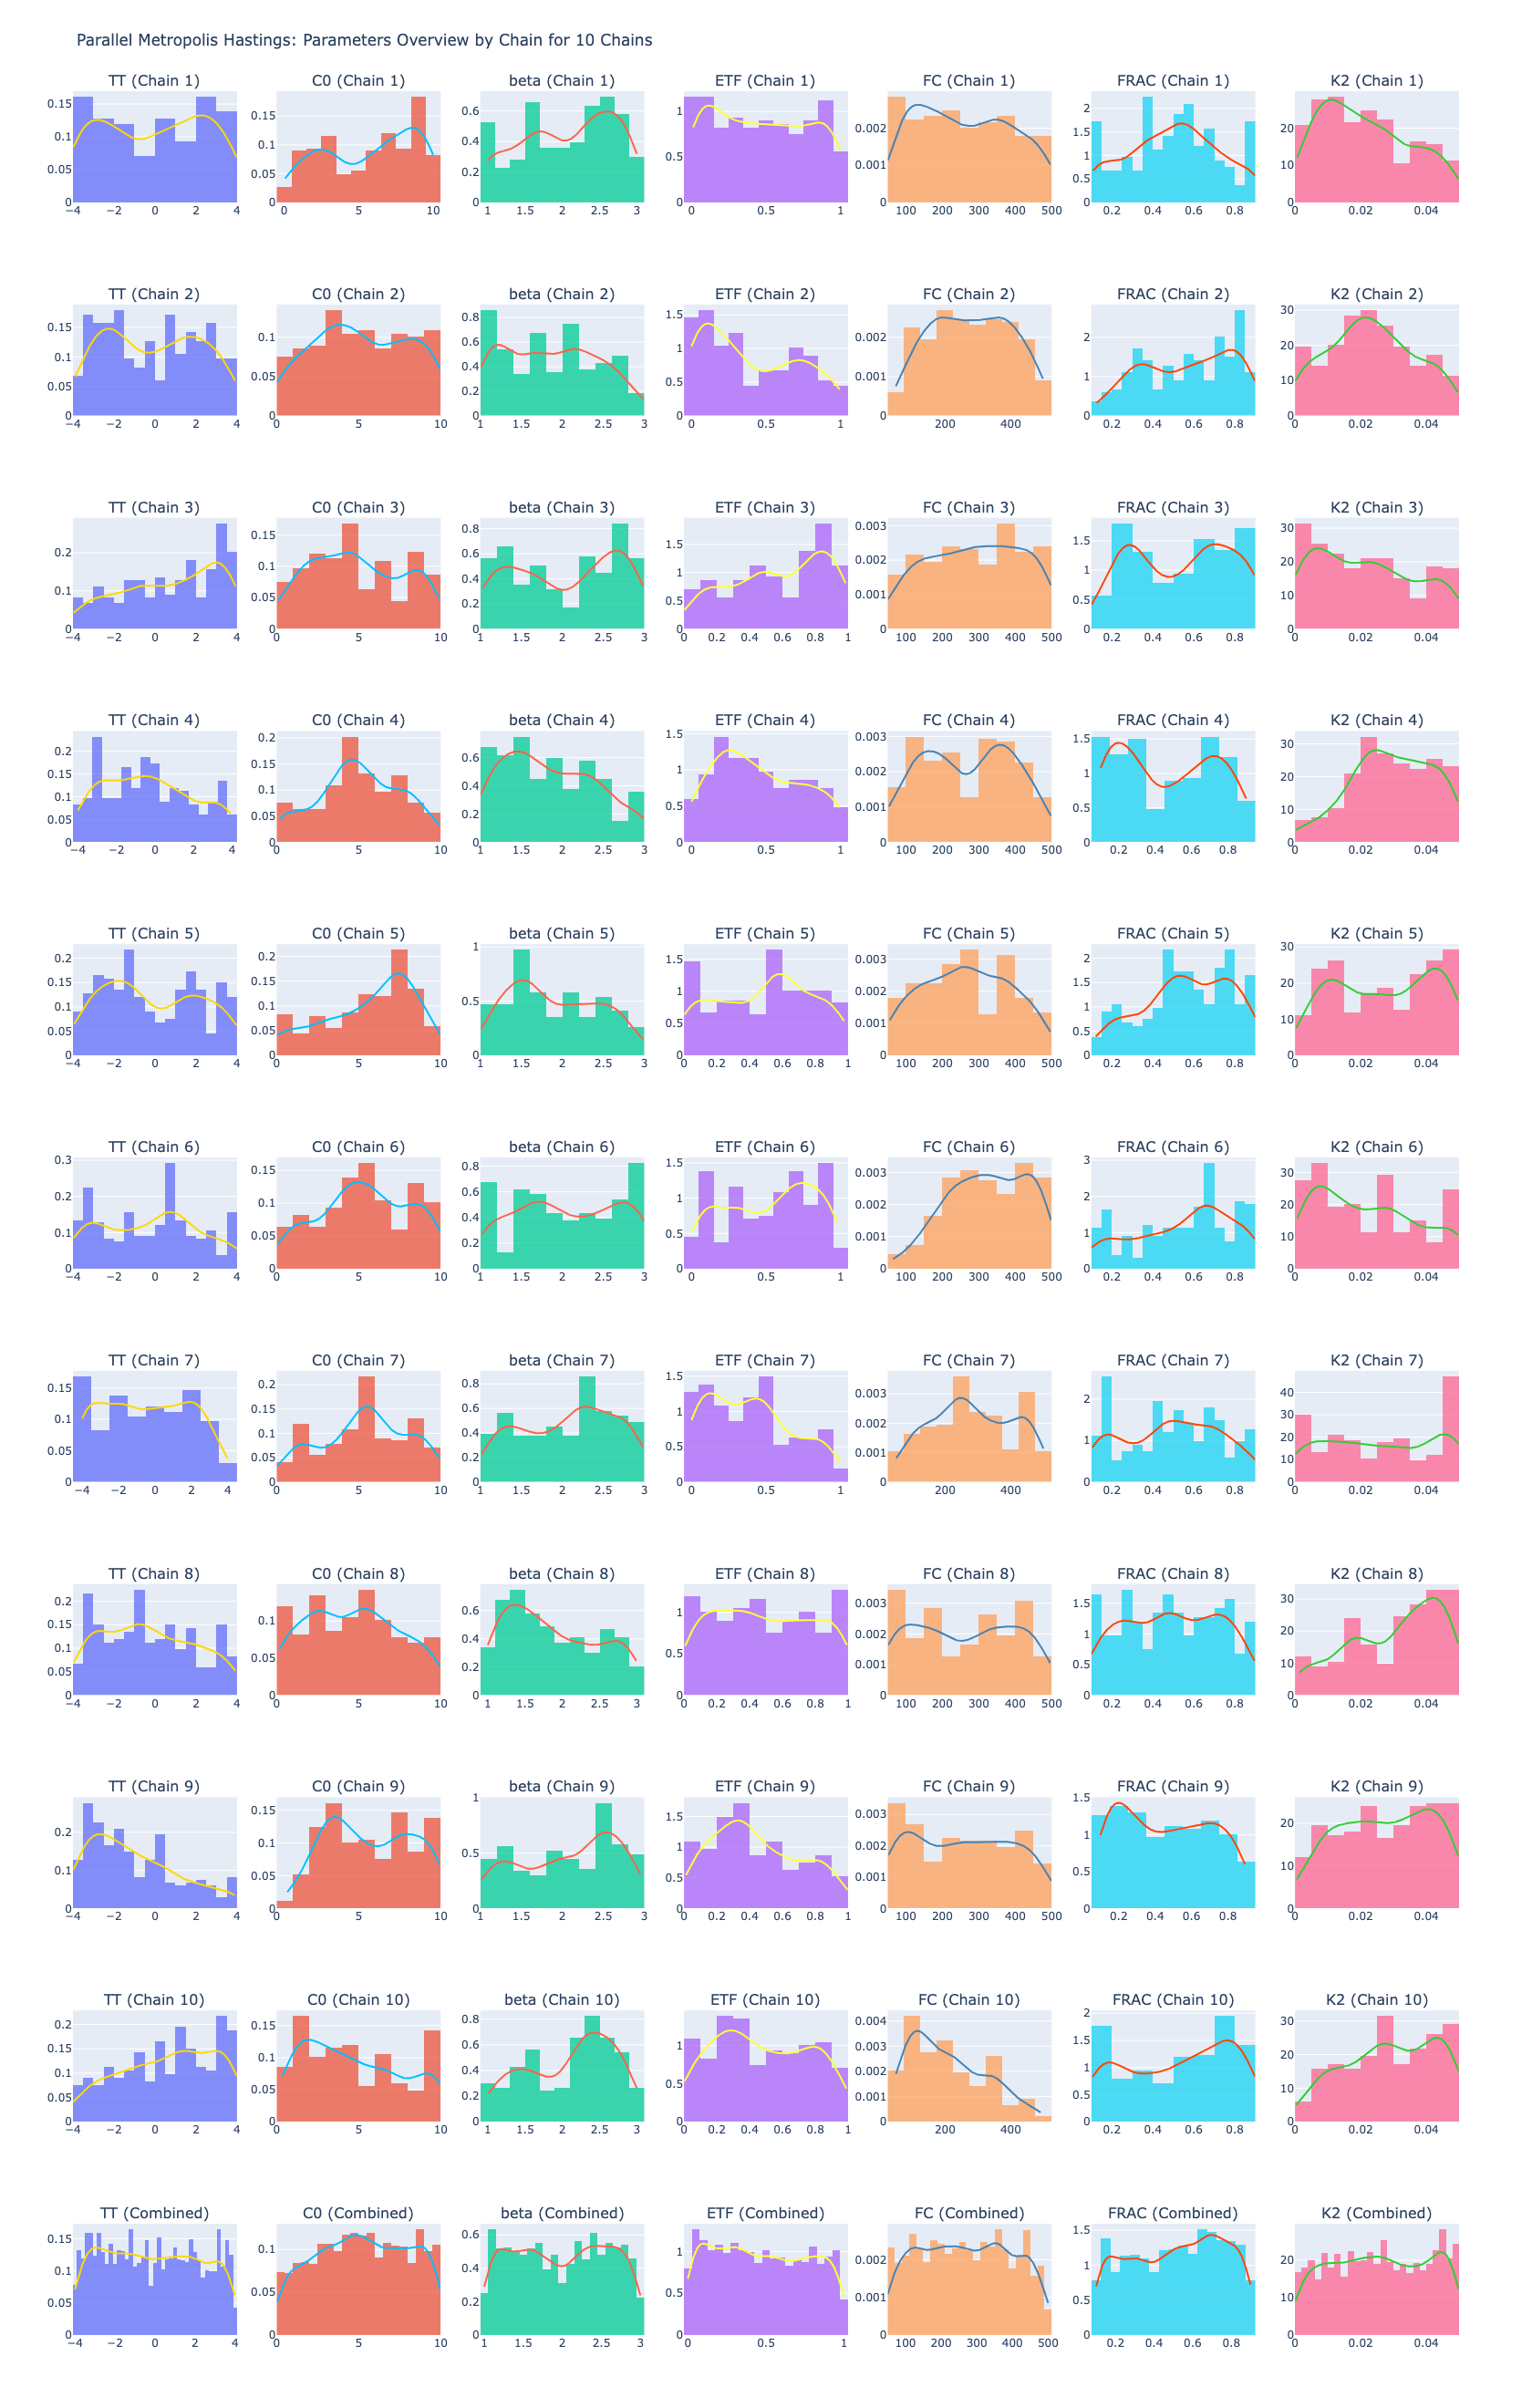
\includegraphics[width=.6\textwidth]{figures/parallel_mh/param_overview_10.png}
    \captionsetup{width=.8\textwidth}
    \caption{Parameter overview by chain for parallel Metropolis Hastings using 10 chains}
    \label{fig:enter-label}
\end{figure}

\begin{figure}[H]
    \centering
    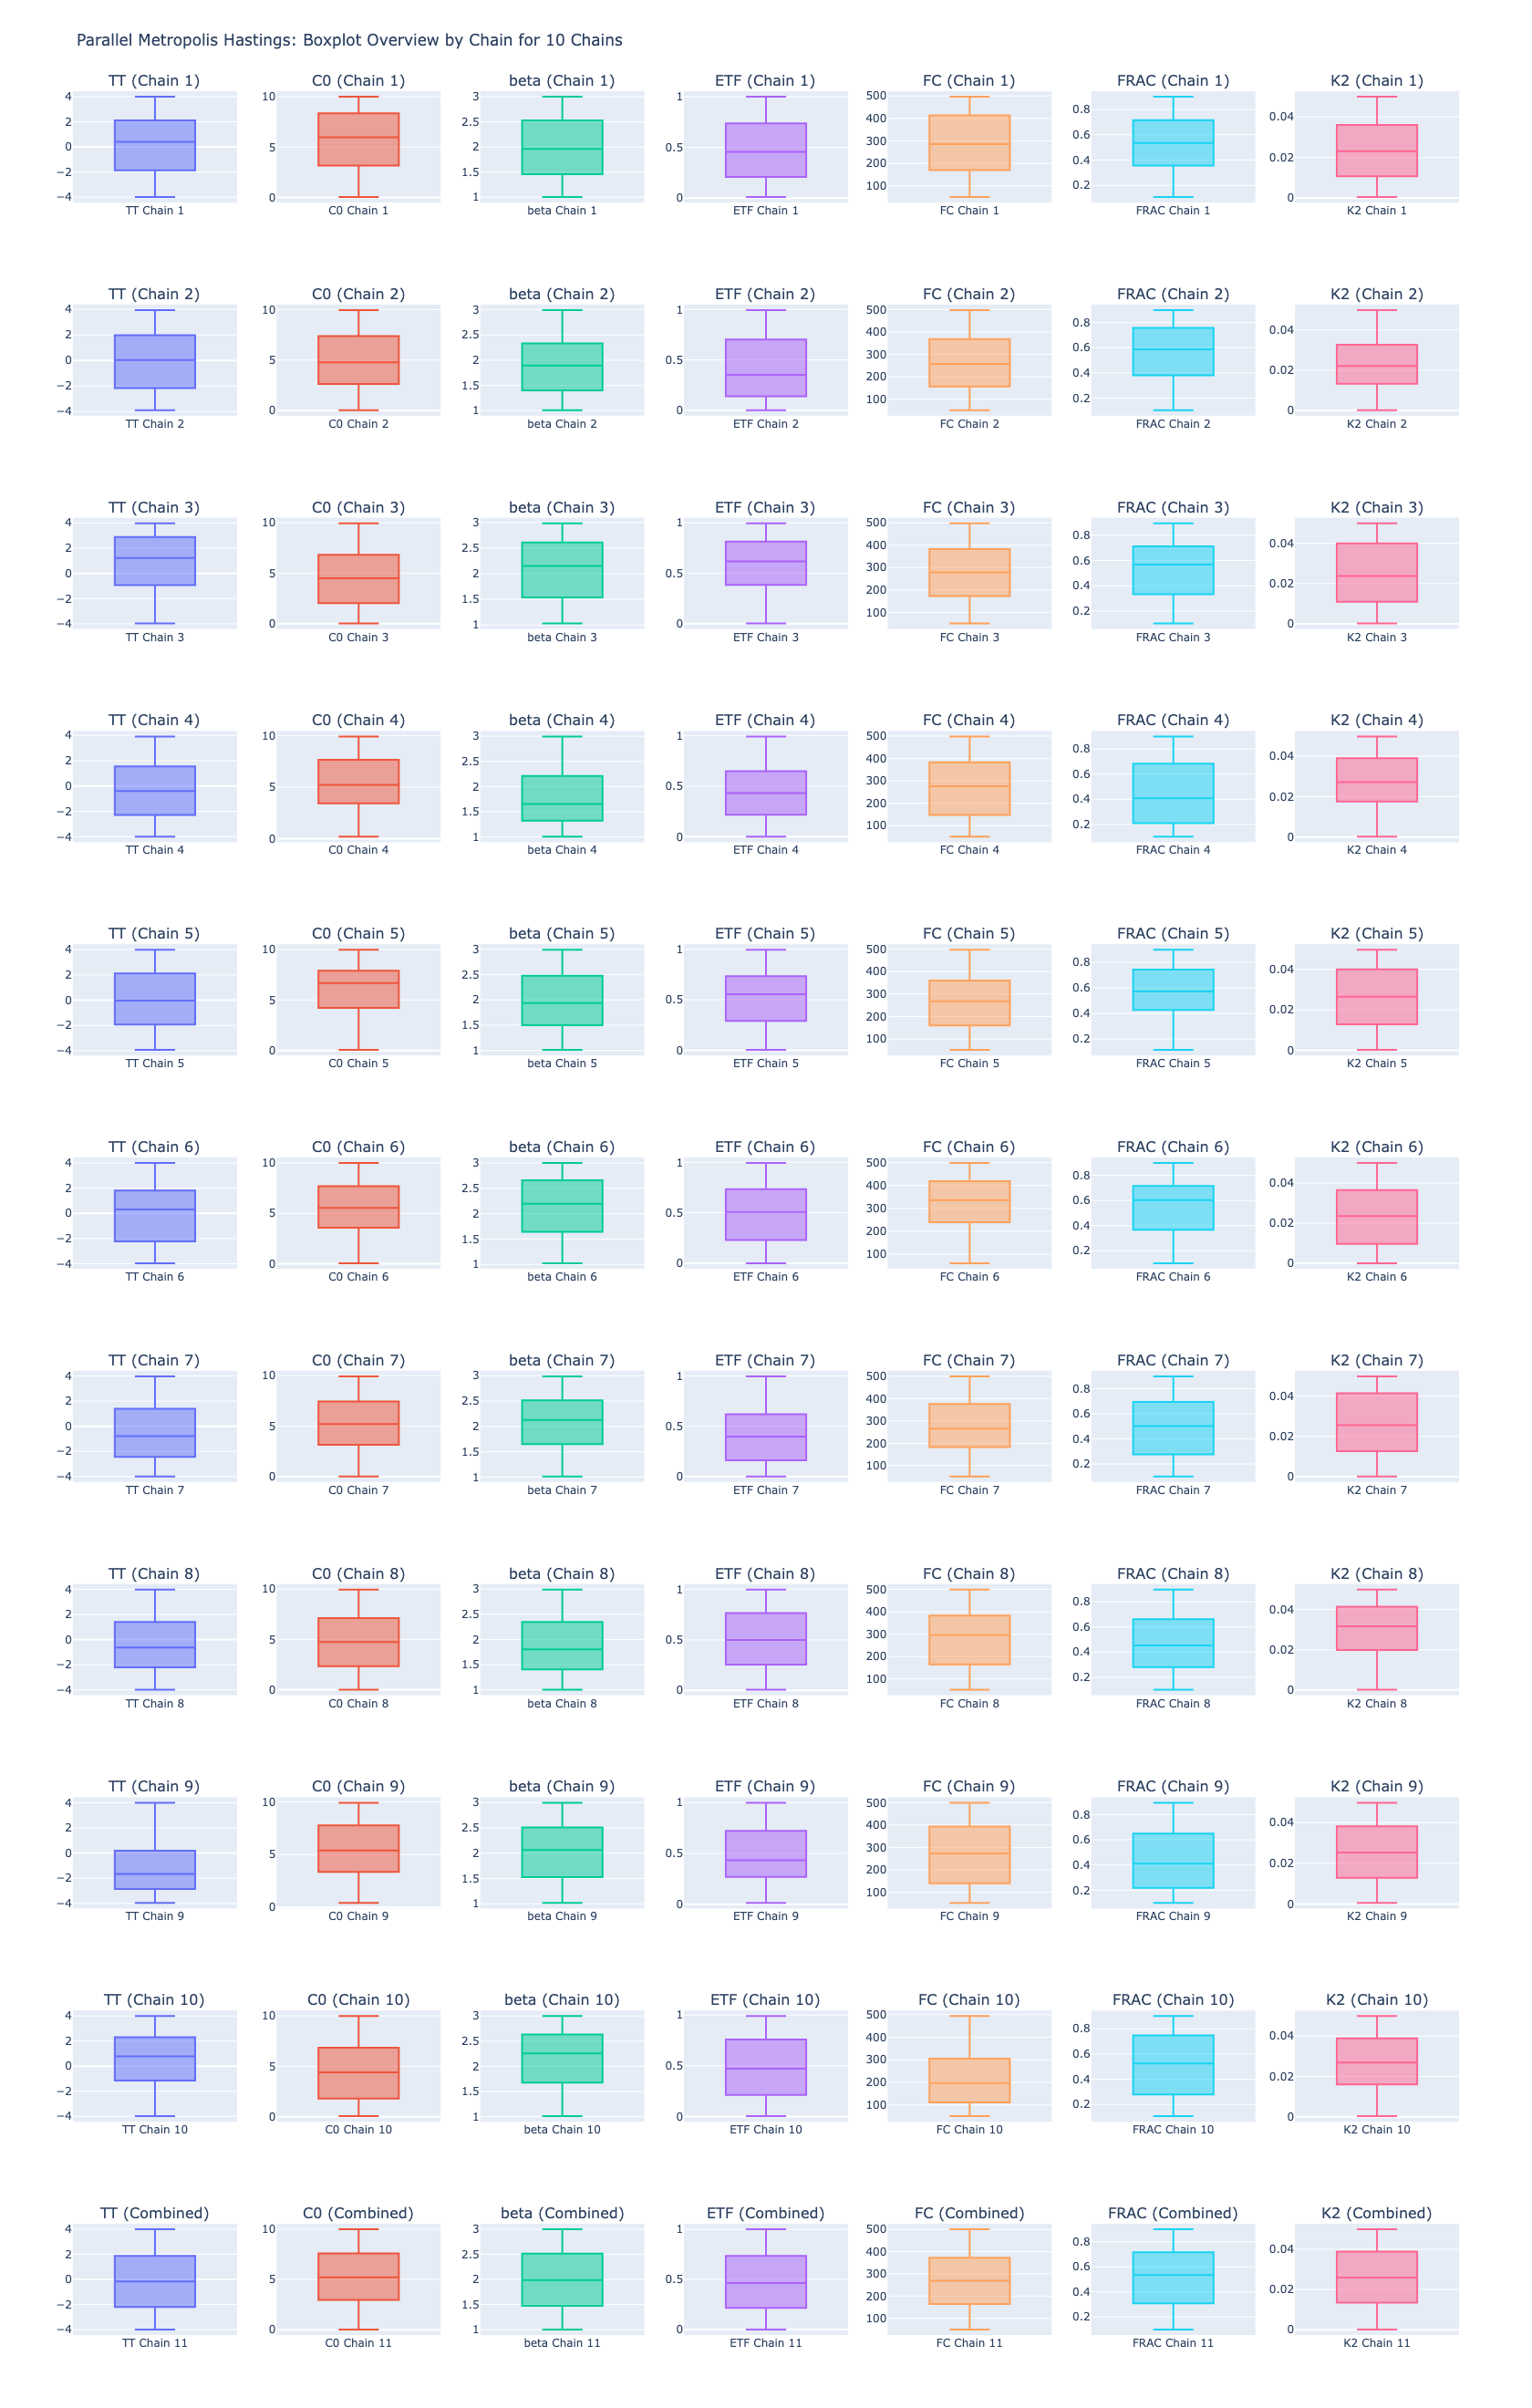
\includegraphics[width=.6\textwidth]{figures/parallel_mh/boxplot_10.png}
    \captionsetup{width=.8\textwidth}
    \caption{Boxplot by chain for parallel Metropolis Hastings using 10 chains}
    \label{fig:enter-label}
\end{figure}

\begin{figure}[H]
    \centering
    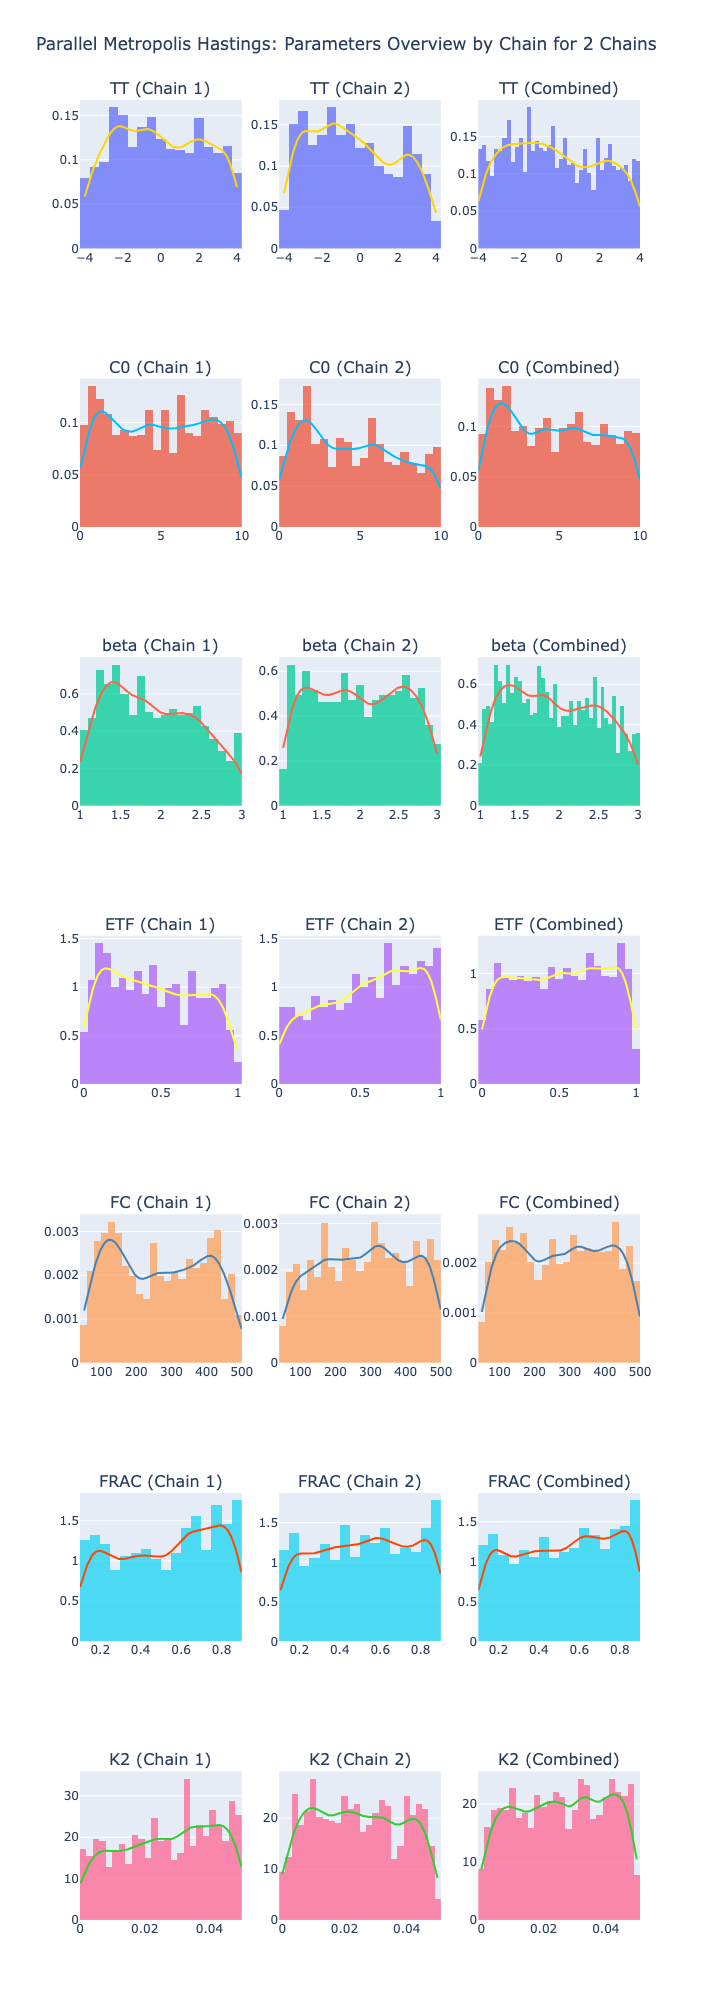
\includegraphics[width=.6\textwidth]{figures/parallel_mh/param_overview_2.png}
    \captionsetup{width=.8\textwidth}
    \caption{Parameter overview by chain for parallel Metropolis Hastings using 2 chains}
    \label{fig:enter-label}
\end{figure}

\begin{figure}[H]
    \centering
    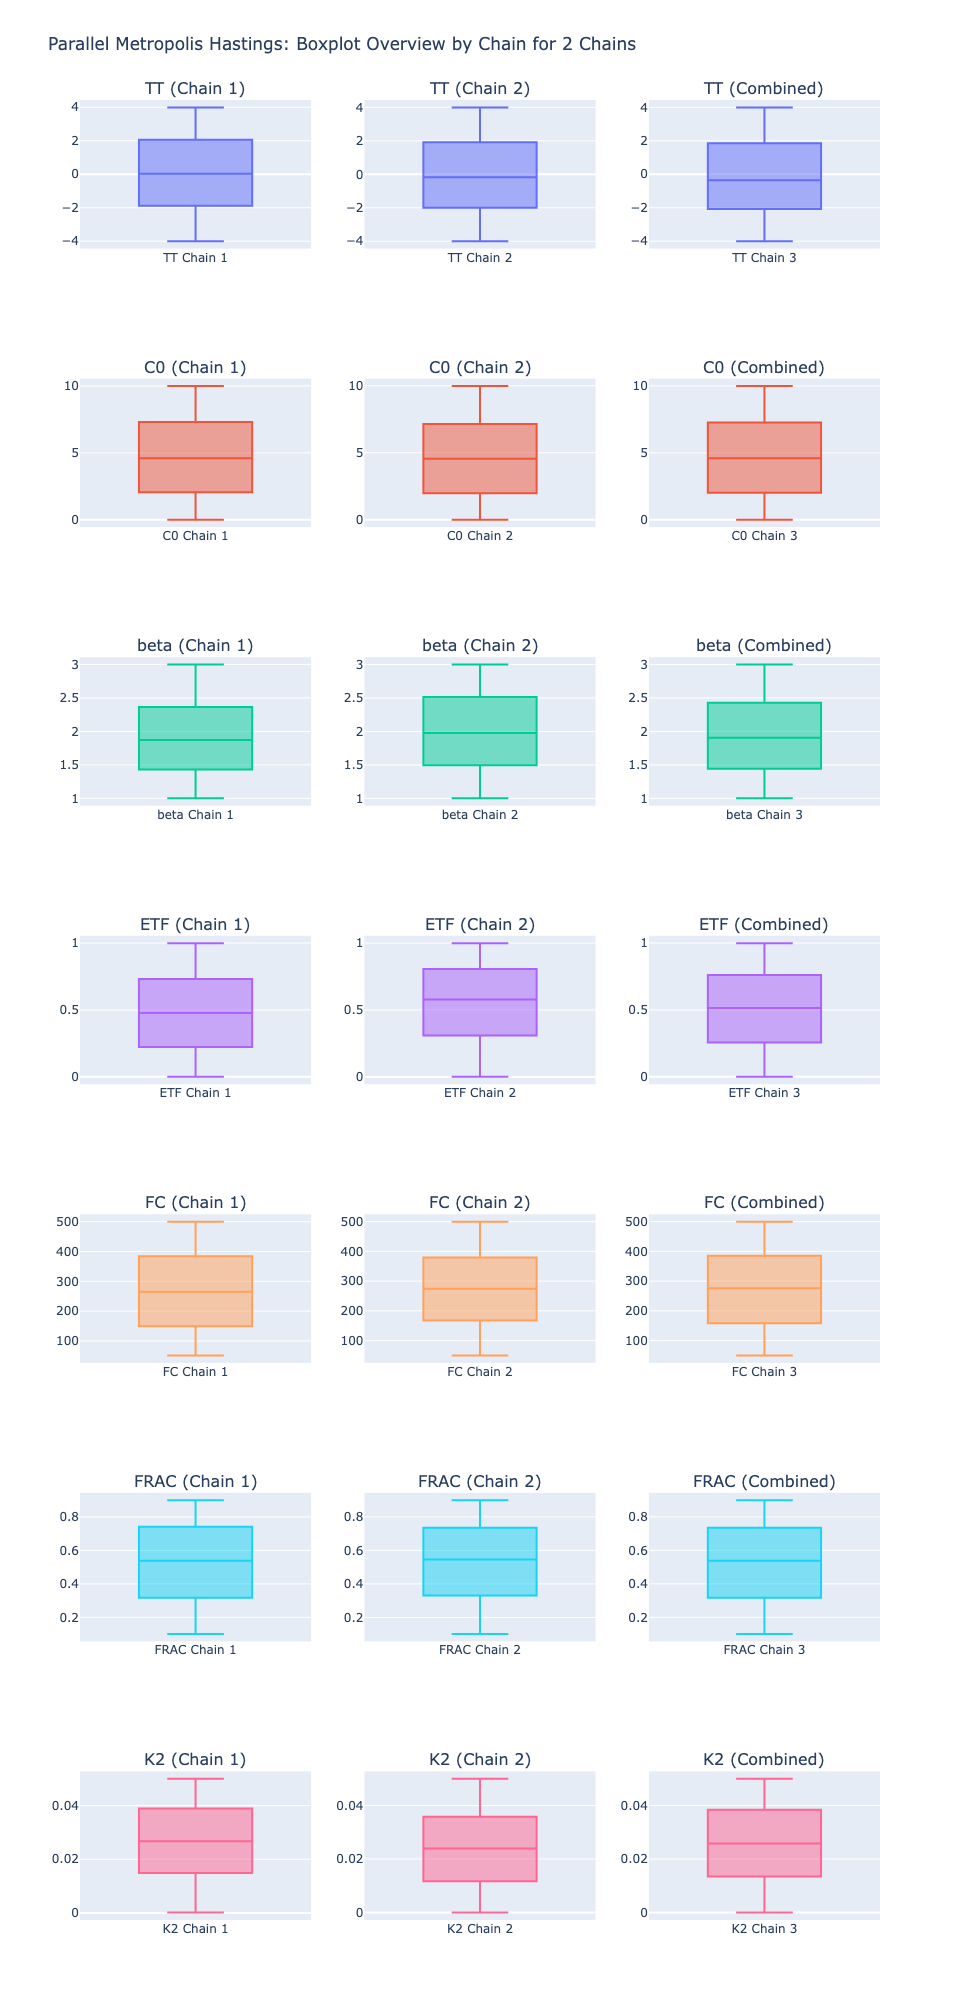
\includegraphics[width=.6\textwidth]{figures/parallel_mh/boxplot_2.png}
    \captionsetup{width=.8\textwidth}
    \caption{Boxplot by chain for parallel Metropolis Hastings using 2 chains}
    \label{fig:enter-label}
\end{figure}
\chapter{General Parallel Metropolis Hastings}

\section{Introduction of the Algorithm}
The general parallel Metropolis Hastings algorithm is an algorithm that is based on the fundamental Metropolis Hastings algorithm with some more parallel modification. Instead of using different chains to make the algorithm to run parallel, the general parallel Metropolis Hastings algorithm applies a different idea: it generates multiple samples instead of one single sample in each iteration. This idea of parallel execution is inspired to avoid sequential generation of data,\cite{gpmh_broshure} which means that instead of accepting or denying the generated sample, a different way to determine the acceptance of the generated sample points needs to be come up. Since the last sample before the generated sample is carried on if the newly generated sample is denied, we also take the last generated sample into account when designing the general parallel Metropolis Hastings. However, since an array of points are generated, we will randomly select one of the samples as the starting point for the next round of generation.\cite{gpmh_derivation} Suppose that we draw $m$ samples in each iteration, we then have to use $m + 1$ samples to perform the acceptance or rejection. What we then do is to randomly sample $n$ points from these $m$ samples. We construct a probability space by calculating the likelihood for each sample points and sample a subset of these points as the points that should be added to the results.

A detailed explanation of the calculation of acceptance probability is inspired from the derivation is from the GMH library of the MUQ framework.\footnote{https://bitbucket.org/mituq/muq2/src/d99f6124bf142922d7973cc60c25d7a518084d12/modules/SamplingAlgorithms/src/GMHKernel.cpp?at=master#GMHKernel.cpp-1,16,45,50,56,58,84} The first step is to construct the acceptance matrix. This matrix has the dimension of  The acceptance probability matrix \( A \) is calculated as follows:

\begin{equation}
A_{ij} = 
\begin{cases} 
\min\left(1, \frac{\exp(r_j - r_i)}{m + 1}\right) & \text{if } i \neq j \text{ and } \text{proposed state } j \text{ is not None} \\
1-\sum_{k \neq i} A_{ik} & \text{if } i = j
\end{cases}
\end{equation}

where $r_j$ is the log density of the $j$th proposed state.

We then calculate the stationary acceptance distribution. It is denoted as $\pi$, which is a vector with length of $m+1$. In order to calculate this, we construct the matrix $M = A^T - I$, on which an extra row of 1 is added at the very bottom that represents the weight of the last generated sample. In order to calculate the stationary distribution, we create the $b$ vector with $0$ everywhere except for the last position, in which a $1$ is set for the same reason mentioned above.\cite{gpmh_derivation} The calculation is then listed as follows:
\begin{equation}
M\pi = b
\end{equation}

After acquiring the acceptance rate vector, we construct a probability space using it, in which we calculate the sum of the vector and then normalize it. Using this vector, we generate $n$ samples from it, including the sample that is generated before. We iterate this process for a certain amount of time and receives the result. To sum up the entire process, we use pseudo code to illustrate it.
\\


\begin{algorithm}[H]
\SetKwFunction{GeneralParallelMetropolisHastings}{GPMH}
\SetKwProg{Fn}{Function}{:}{}
\KwIn{\tabto{2cm}proposal distribution function, sampling kernel function, likelihood kernel function, initial state, number of iterations, acceptance\_rate\_calculation, num\_proposals, num\_accepted}
\KwOut{\tabto{2cm} list of sampled data points}
\BlankLine

\Fn{\GeneralParallelMetropolisHastings{proposal\_dist, sampl\_kernel, likel\_kernel, init\_state, iterations, acceptance\_rate\_calculation, num\_proposals, num\_accepted}}{
    \tcp{Initialize the samples list with the initial state}
    samples $\leftarrow$ [init\_state]
    old $\leftarrow$ init\_state
    
    \For{i $\leftarrow$ 1 \KwTo iterations}{
        \tcp{Generate a new sample from the sampling kernel}
        generated_samples $\leftarrow$ [old] \\

        \For{j $\leftarrow$ 1 \KwTo num\_proposals}{
            generated_samples.append(sampl\_kernel(old))\\
        }
        
        \tcp{Calculate the acceptance probability}
        acceptance\_rates = acceptance\_rate\_calculation(generated_samples)
        
        \tcp{Decide to accept or reject the new sample}
        \tcp{random\_sampling is a function that takes two parameters, sampling randomly the number of times given in the first parameter from the array given in the second parameter using the acceptance rate provided in the third parameter}
        res $\leftarrow$ random\_sampling(num\_accepted, num\_proposed, acceptance\_rates)
        samples.append(res)
        old = random(res)
    }
    \Return samples
}

\caption{General Parallel Metropolis-Hastings Algorithm}
\end{algorithm}


\section{Evaluation}
After discussing the algorithm itself, we run the algorithm and generate data that can be used to analyze. In this section, we will first try to observe the algorithm regarding the number of samples generated and accepted in each iteration through ratio and amount test. Afterwards, further investigation regarding input parameters are conducted.

\subsection{Ratio Test}
The very first test for evaluation is called the ratio test. In this test, we investigate the ratio between the numbers generated and numbers accepted. This test is conducted in order for us to find the most optimal ratio of both parameters for the Bayesian inference problem. We fix the numbers of the accepted samples being five, while the numbers of generated sample being a variable. The tested scenarios include: 5 generated samples for ratio of 1, 10 generated samples for ratio of 2, 20 generated samples for ratio of 4, 40 generated samples for ratio of 8, 80 generated samples for ratio of 10. As we can see from the figure 6.1, the accuracy of the Bayesian inference goes up as the ratio of the generated sample amount against the accepted sample amount goes up. The larger the ratio is, the more accurate the Bayesian inference would be. However, the trade off would be the run time, as the run time grows. There is an obvious exponential relationship between the run time and the ratio. Therefore, we need to consider the trade off between accuracy and efficiency while selecting an appropriate ratio.

\begin{figure}[H]
    \centering
    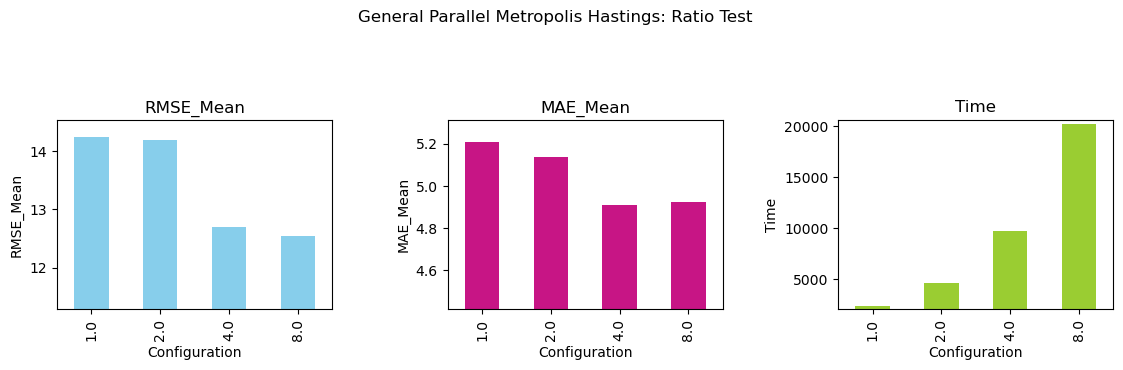
\includegraphics[width=1\textwidth]{figures/gpmh/ratio_test.png}
    \captionsetup{width=.8\textwidth}
    \caption{}
    \label{fig:enter-label}
\end{figure}

\subsection{Amount Test}
We move on to the amount test, in which we investigate an optimal amount of samples that needs to be generated for each iteration. We fix the ratio between the generated samples and the accepted samples being $2$. The tested scenarios include: 10 generated samples with 5 being accepted, 20 generated samples with 10 being accepted, 40 generated samples with 20 being accepted, 80 generated samples with 40 being accepted and 100 generated samples with 50 being accepted. In comparison with the ratio test, the differences are not that obvious in this case. For the RMSE, better performances of the Bayesian inference are delivered for higher amounts, whereas the MAE data does not differ too much from each other. For the efficiency, faster execution happens also in higher ranges of amount numbers. Therefore, the more samples generated in each iteration, the faster and more accurate the algorithm will be.

\begin{figure}[H]
    \centering
    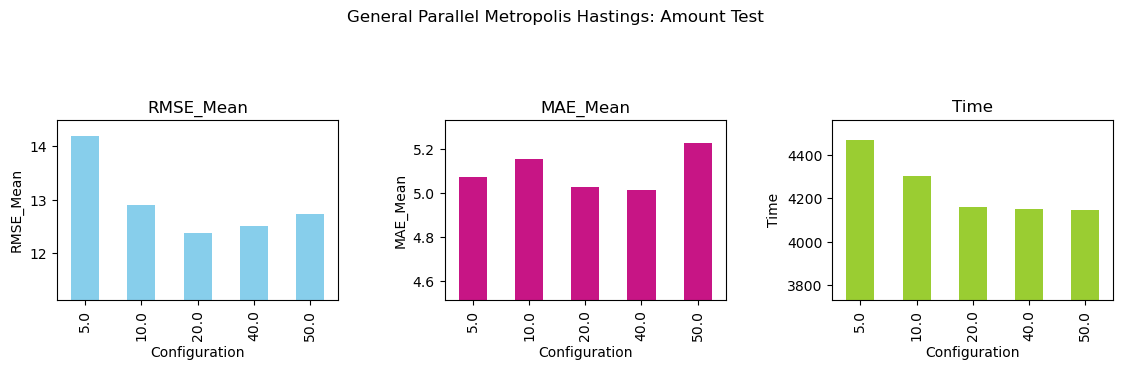
\includegraphics[width=1\textwidth]{figures/gpmh/amount_test.png}
    \captionsetup{width=.8\textwidth}
    \caption{}
    \label{fig:enter-label}
\end{figure}

\subsection{Sampling out of bounds}
After investigating the relationship between generated sample numbers and the accuracy and efficiency metrics, we now switch gears to the input parameters. For the first input parameter, we take a look at the sampling out of bounds methods. As it was mentioned before, we apply three methods when handling samples that are generated out of bounds: ignoring, reflect boundary and aggregation. These three methods are also used in general parallel Metropolis Hastings algorithm. The benchmark result is shown in figure 6.x. Unlike the case in the fundamental implementation, all these three variants show little difference from each other in terms of accuracy. In terms of efficiency, the ignoring method still outperforms the other two methods just like the case for the fundamental implementation, however not by a lot. The selection of the method usage is therefore not the most relevant selection for the general parallel Metropolis Hastings algorithm considering the minimal impact on the accuracy and efficiency metrics.

\begin{figure}[H]
    \centering
    \includegraphics[width=1\textwidth]{figures/gpmh/sotb.png}
    \captionsetup{width=.8\textwidth}
    \caption{}
    \label{fig:enter-label}
\end{figure}

\subsection{Initial States}
Another input parameter that might impact the result outcome is the initial states. The selection of initial state does not result in drastic difference in the accuracy metrics for the fundamental Metropolis Hastings, and it is exactly the case here. For both metrics, the value for each input option of initial states does not vary much from each other. For the efficiency, on the other hand, the initial state had a drastic influence on the run time. The fundamental algorithm with the best initial state could achieve less than twice of the time of which with the worst initial state. This is the complete opposite for the general parallel Metropolis Hastings algorithm, in which algorithms with all different selections of initial states deliver similar results, all with run time around 4000 seconds. This means that the selection of initial state does not have a big influence on the overall result of the general parallel Metropolis Hastings algorithm. 

\begin{figure}[H]
    \centering
    \includegraphics[width=1\textwidth]{figures/gpmh/init_states.png}
    \captionsetup{width=.8\textwidth}
    \caption{}
    \label{fig:enter-label}
\end{figure}

\subsection{Dependent Likelihood Kernel Factor}
The behavior of the dependent likelihood kernel factor for the general parallel Metropolis Hastings algorithm is far different from the one for the fundamental Metropolis Hastings algorithm. For the case here, the accuracy shows a certain level of irregularity, with the value $0.6$ delivering the most optimal result. For the efficiency, on the other hand, every run using different input values result in almost the same run time, with the exception of $0.8$ as an anomaly, requiring more time than any other input values. Therefore, the value $0.6$ is the most optimal choice for this case here.

\begin{figure}[H]
    \centering
    \includegraphics[width=1\textwidth]{figures/gpmh/dependent_likelihood_kernel_factor.png}
    \captionsetup{width=.8\textwidth}
    \caption{}
    \label{fig:enter-label}
\end{figure}


\subsection{The Rest of Input Parameters}
For the rest of the input parameters, detailed explanations are spared for this chapter, since they have the similar results as the fundamental Metropolis Hastings algorithm. These are listed here as follows: 
\begin{itemize}
    \item Transition kernel factor: Not many differences in terms of accuracy. For the efficiency part, the run time of the algorithm does not matter from each other too much, apart from an anomaly point at the very last, which has also occurred in the fundamental Metropolis Hastings algorithm.
    \item Independent likelihood kernel factor: there is a peak on which the accuracy performance is the worst, $3$ in the case of general parallel Metropolis Hastings. Centered from this peak, the result gradually becomes more accurate. The run time for each run does not differ from each other by much.
    \item Dependent likelihood kernel factor:
    \item Burn in: No big differences of both metrics across different input values.
    \item Effective Sample Size: No big differences of both metrics across different input values.
\end{itemize}

\section{Comparison of General Parallel Metropolis Hastings with the Fundamental Implementation}
After performing analysis on the general parallel Metropolis Hastings algorithm, a comparison of it and the fundamental Metropolis Hastings algorithm is made here. For most cases, the RMSE score of the algorithm is around $12$ and the MAE score is around $5$. This improves significantly from the fundamental Metropolis Hastings algorithm, which delivers an RMSE score of around $20$ and an MAE score of around $9$. However, the fastest run of the fundamental Metropolis Hastings algorithm is around $1400$ seconds in comparison of around $4000$ seconds of the general parallel Metropolis Hastings algorithm. Between better efficiency and better accuracy, there is a trade off that needs to be considered.
\chapter{The DREAM Algorithm}
The DREAM algorithm is a Markov Chain Monte Carlo method that is designed for efficient sampling from complex and high-dimensional probability distributions. 

In this chapter, the algorithm is applied to the hydrological model. The output will then be analyzed and compared to the models from the chapters above.

\section{Algorithm Introduction}
The DREAM algorithm is designed based on the fundamental Metropolis-Hastings algorithm and the possibility of parallel execution of the algorithm. It applies differential evolution. It utilizes multiple Markov chains running in parallel to explore the parameter space. Proposals for new sample points are generated using the differences between pairs of chains. This differential evolution property helps to enhance sampling efficiency and convergence. 


In the first section, we break down the DREAM algorithm step by step with details explained for individual components.\cite{dream} First, we take a look at the function header. Information regarding input parameter requirements should be provided.

\begin{algorithm}[H]
function $[x, p_X]$ \gets \textbf{DREAM}$(prior, pdf, N, n, T, d)$
\end{algorithm}

The DREAM algorithm takes in several parameters as input. These include:
\begin{itemize}
    \item $prior$: The prior distribution of the parameter space
    \item $pdf$: The probability density function
    \item $N$: Number of chains
    \item $n$: Number of generations
    \item $T$: Thinning factor, which is the implementation of effective sample size in the DREAM algorithm. Only the $T$-th sample will be retained in order to reduce autocorrelation\cite{dream}
    \item $d$: Dimension of the inferred parameter space
\end{itemize}
The output would include $x$, which is the sampled chains positions, and their probabilities, which is denoted by $p_X$.

We move on to the next step, in which variables are initialized.\\

\begin{algorithm}[H]
$[delta, c, c\_star, n\_CR, p\_g] \gets [3, 0.1, 1e-12, 3, 0.2]$\\
$x \gets \textbf{zeros}(T, N, d)$\\
$p\_X \gets \textbf{zeros}(T, N)$\\
$[J, id] \gets [\textbf{zeros}(1, N), 1:N]$\\
\For{$i \gets 1$ \kwTo $N$}{
   $R(:, (i-1) * N + (1:N)) \gets \textbf{setdiff}(1:N, i)$\\
}
$CR \gets [1:n\_CR] / n\_CR$\\
$pCR \gets ones(1, n\_CR) / n\_CR$\\
\end{algorithm}

In this part, most variables that are internally used in this algorithm and not passed as the input parameters are initialized. These include:
\begin{itemize}
    \item $delta$: Number chain pairs proposal. As mentioned in the introduction of this chapter, this value is used for observing the differential evolution of the sample space
    \item $p\_g$: The probability of selecting a specific number of pairs of chains for generating the proposals
    \item $c$: The scaling factor that controls the step size of the proposal distribution
    \item $c\_star$: The parameter that is used to adaptively update the scaling factor $c$ during sampling, so that an optimal acceptance rate can be controlled
    \item $J$: The jump rate. It measures the average distance between successive samples in the parameter space and thus quantifies the effectiveness of the parameter space exploration
    \item $id$: Chain indices that correspond the jump rate
    \item $CR$: The crossover rate. It is used to determine the proportion of dimensions in which the state of the generated sample differs from the current state
    \item $n\_CR$: The number of different crossover values. It allows for adaptive updating of the crossover rates during sampling
    \item $pCR$: The probability of each crossover rate being selected
\end{itemize}

Next up, we initialize the sample states and probabilities.\\
\begin{algorithm}[H]
$X \gets \textbf{prior}(X, d)$\\
\For{$i \gets 1$ \kwTo $N$}{
    $p\_X(i, 1) \gets pdf(X(i, :))$
}
$x(1, :, 1:d) = \textbf{reshape}(X', [1, N, d]); p\_X(1, 1:N) = p_X'$
\end{algorithm}

In this segment, the initial states are generated from the prior distribution and stored in $X$. The initial probability of each chain is also computed using the $pdf$ function and stored in $p_X$. They are then reshaped correspondingly.

From now on, the algorithm enters the sample generation phase. It repeats itself until the completion of sample generation. All of the segments below are wrapped inside of a for loop that repeats until $n$ cycles, which is the number of generation steps. The first segment inside of the loop looks like this:

\begin{algorithm}[H]
$ draw \gets \textbf{sort}(\textbf{rand}(N-1, N))$\\
$dX = \textbf{zeros}(N, d)$\\
$lambda = \textbf{unifrnd}(-c, c, N, 1)$
$std\_X = std(X)$
\end{algorithm}

The $\textbf{unifrnd}$ function is a function that generates random numbers from a uniform distribution. Here, we instantiated another few internal variables.
\begin{itemize}
    \item $draw$: A list of random numbers, used to determine the order of chain updates
    \item $dX$: An array to store proposal differences.
    \item $lambda$: A random variable sampled from a uniform distribution between \(-c\) and \(c\), used for adaptive scaling of the proposal step size.
    \item $std_X$: The standard deviation of $X$, used later for adaptive scaling.
\end{itemize}

Moving on to the next segment, we generate the proposals.

\begin{algorithm}[H]
\For{$i \gets 1 \kwTo N$}{
    $D \gets \textbf{randsample}([1:delta], 1)$\\
    $a = R(i, draw(D, 1))$\\
    $b = R(i, draw(D+1:2*D, 1))$\\
    $d = \textbf{randsample}(1:n_CR, 1, pCR)$\\
    $z = \textbf{rand}(1, d)$
    $A = find(z <= CR(d))$
    \If{$len(A) == 0$}{
        $A \gets min(z, c\_star = 1)$
    }
    $gamma\_d = 2.38 / sqrt(2 * len(A) * p\_g * (1 - p\_g))$
}
\end{algorithm}

The algorithm loops through every single chain and draws proposals.
\begin{itemize}
    \item $D$: Selects a number of differences for the proposal generation
    \item $a$, $b$: Chain indices, used in the differential evolution proposal
    \item $d$: Selects a crossover rate using probabilities $pCR$
    \item $A$: Determines the dimensions that are involved in the crossover. If the dimension turns out to be $0$, we enforce $1$ to be the minimum dimension size
    \item $gamma\_d$: The scaling factor for the differential evolution proposal. The calculation is based on the number of dimensions and a probability factor $p_g$.
\end{itemize}

For the next step, the algorithm focuses on the differential evolution proposal. This is one of the most crucial steps of the DREAM algorithm, making it different from other Markov chain Monte Carlo algorithms.

\begin{algorithm}[H]
$g \gets \textbf{randsample}([gamma\_d, 1], 1, [1-p\_g, p\_g])$\\
$dX(i, A) = c\_star + randn(1, len(A)) + (1 + lambda(i)) * g * sum(X(a, A) - X(b, A))$\\
$Xp(i, 1:d) \gets X(i, 1:d) + dX(i, 1:d)$\\
$p\_Xp(i, 1) \gets pdf(Xp(i, :))$\\
$p\_acc \gets \textbf{min}(1, p\_Xp(i, 1) / p\_X(i, 1))$
\end{algorithm}

In this segment, a few calculations is done to decide whether to accept the proposed move. This is done by generating a uniformly distributed random number and accepting the proposed state if this number is less than or equal to the calculated acceptance probability, namely $p_{acc}$.

\begin{itemize}
    \item $g$: Selects a number from $gamma_d$ or 1
    \item $dX$: The actual differential evolution proposal, calculated based on the dimension count of $A$, the variability term $lambda$ that is defined above, and the $g$ selected in the row above
    \item $Xp$: The newly proposed positions
    \item $p\_Xp$: Density of the newly proposed positions
    \item $p\_acc$: The acceptance probability, calculated based on the newly proposed positions and their corresponding probabilities using the Metropolis criterion as the fundamental Metropolis Hastings algorithm
\end{itemize}

Afterward, we accept or reject the samples that are generated, the same as any other Markov chain Monte Carlo algorithm.

\begin{algorithm}[H]
\If{$rand < p\_acc$}{
    $x(i, 1, :) \gets Xp(i, :)$
    $p\_X(i, 1) \gets p\_Xp(i, 1)$
}
\Else{
    $dX(i, 1:d) \gets 0$
}
$J(i) \gets J(i) sum((dX(i, 1:d) ./ std_X).^2)$
$id(i) \gets id(i) + 1$
\end{algorithm}

The process of this step is relatively straightforward. A random number is drawn, so that the algorithm can decide if the proposal is accepted. If the proposal is accepted, the position and density of the chain are updated. Otherwise, $dX$ is reset to zero for that chain. Afterwards, the jump rate $J$ and chain index $id$ are updated.

Before ending the repetition and continuing with the next step, there is an extra step in the DREAM algorithm which involves chaining and mixing.

\begin{algorithm}[H]
$x(:, :, :) \gets \textbf{reshape}(X(:, 1:d), [], N, d)$\\
$p\_X(:, 1:N) \gets p\_X.\textbf{transpose}$\\\
\If {$t < T /10$}{
    $pCR \gets 1./J$
    $pCR \gets pCR / \textbf{sum}(pCR)$
}
$[x, p\_X] = \textbf{check}(X, \textbf{mean}(\textbf{log}(p\_X(\textbf{ceil}(T/2):T, :))))$
\end{algorithm}
What the algorithm does in this part is to reshape and update the density of the chain's position for the next iteration. The crossover probabilities $pCR$ are then updated based on the jump rate $J$ to enhance mixing. At the very end, a check function is used to perform outlier detection based on the log probabilities of the chains, removing them and leaving the valuable data inside of the variable.

The loop is then ended. The final step of the algorithm is self-explanatory, namely the return phase. It returns the sampled values in the form of chains and ends itself.
\begin{algorithm}
    $\textbf{return}\  x, p\_x$
\end{algorithm}

The algorithm itself is originally implemented using MATLAB, though it is later rewritten and offered in multiple packages with different implementation variants. For this thesis, the PyDREAM library\footnote{https://pydream.readthedocs.io/en/latest/index.html} is selected for use. The PyDREAM library brings the DREAM algorithm to the platform of Python with easy installation and usage,\cite{pydream} which is optimal for the use case of this thesis.

\section{Evaluation Based on Chains}
For the DREAM algorithm, there is a set of default input parameters. Therefore, before exploring the influence of the input parameters on the actual output, we first use this set of default input parameters to run the algorithm to observe how the output of the Bayesian inference looks. Since it is an algorithm based on chains, we analyze the sampled results both with and without regard to chains, analogous to the parallel Metropolis-Hastings algorithm. For the test cases, we test the algorithm using $10$, $8$, $5$, and $4$ chains. Numbers of chains lower than $4$ are not possible due to the policy of the DREAM algorithm, stating that the chain amount must be greater than twice the value of DEpairs + 1. The DEpairs parameter describes the pair of differential evolution and ensures there are enough chains to form the required number of DE pairs for proposal generation.


\subsection{Efficiency}
First, we take a look at the efficiency of the algorithm. We measure the run time for different test cases regarding chain amounts and compare them using graphics, which are displayed below in Figure 7.1. Unlike the parallel Metropolis-Hastings algorithm, there is no strict correlation that can be found between the number of chains and the run time of the DREAM algorithm. The cause is that instead of treating different chains individually, the DREAM algorithm uses cross-over calculations to track the relationships between the different chains. Therefore, the additional calculation results in the irregularity of the efficiency across different test cases of chain amounts.

\begin{figure}[H]
    \centering
    \includegraphics[width=1\textwidth]{figures/dream/runtime.png}
    \captionsetup{width=.8\textwidth}
    \caption{Relationship between run time and chain numbers for the DREAM algorithm}
    \label{fig:enter-label}
\end{figure}
\subsection{Trace Plot}
Similar to the case for the parallel Metropolis-Hastings algorithm evaluation, we use the trace plot to track the positioning of generated samples in each step. For the DREAM algorithm, we also analyze the trace plot of both extreme cases, namely the DREAM algorithm run with $10$ chains and $4$ chains. The trace plots of two random chains picked from both cases are shown in Figures 7.2 to 7.5. Visualizations for both cases do not differ much from each other in terms of sampling from the stationary distribution. All parameters in both graphs show apparent convergence approaching the end, where the stationary distribution can be easily observed. We could conclude that the property of sampling from the stationary distribution of individual chains exists and does not need further investigation.

Unlike the observation made for the parallel Metropolis-Hastings algorithm, the DREAM algorithm displays a heavy stationary distribution, where there are far fewer movements, more rejections during the sampling process, and no obvious moving patterns of the traces. Also, the visualizations show that the parameter space of the stationary distribution from the DREAM algorithm is normally a subset of the entire parameter space, which provides a more stable and consistent sampling, unlike the wide parameter sample space exploration upon stationary distribution in the case of parallel Metropolis-Hastings. In conclusion, the DREAM algorithm has a stronger convergence for the sampling process than other Markov chain Monte Carlo algorithms.

\begin{figure}[H]
    \centering
    \includegraphics[width=0.9\textwidth]{figures/dream/tp_rand_10_3.png}
    \captionsetup{width=.8\textwidth}
    \caption{Trace plot of the third chain from the DREAM algorithm with 10 chains}
    \label{fig:enter-label}
\end{figure}

\begin{figure}[H]
    \centering
    \includegraphics[width=0.9\textwidth]{figures/dream/tp_rand_10_7.png}
    \captionsetup{width=.8\textwidth}
    \caption{Trace plot of the seventh chain from the DREAM algorithm with 10 chains}
    \label{fig:enter-label}
\end{figure}

\begin{figure}[H]
    \centering
    \includegraphics[width=0.9\textwidth]{figures/dream/tp_rand_4_1.png}
    \captionsetup{width=.8\textwidth}
    \caption{Trace plot of the first chain from the DREAM algorithm with 4 chains}
    \label{fig:enter-label}
\end{figure}

\begin{figure}[H]
    \centering
    \includegraphics[width=0.9\textwidth]{figures/dream/tp_rand_4_3.png}
    \captionsetup{width=.8\textwidth}
    \caption{Trace plot of the third chain from the DREAM algorithm with 4 chains}
    \label{fig:enter-label}
\end{figure}

\subsection{Gelman Rubin Convergence}
The Gelman Rubin statistic in the case of DREAM is generally higher than the convergence diagnostic of the general parallel Metropolis-Hastings algorithm, even though the convergence statistic is generally in the acceptable range below $1.2$. The figures for all test cases are displayed in Figures 7.6 to 7.9. For the case of 10 chains, two parameters show relatively high convergence diagnostic values that almost exceed the threshold. For other cases, there are also some parameters that show higher convergence diagnostic values than others. However, no specific patterns or regularities can be found for the Gelman-Rubin convergence parameter. 

\begin{figure}[H]
    \centering
    \includegraphics[width=1\textwidth]{figures/dream/gr_10.png}
    \captionsetup{width=.8\textwidth}
    \caption{Gelman Rubin Convergence Diagnostic of the DREAM algorithm with 10 chains}
    \label{fig:enter-label}
\end{figure}

\begin{figure}[H]
    \centering
    \includegraphics[width=1\textwidth]{figures/dream/gr_8.png}
    \captionsetup{width=.8\textwidth}
    \caption{Gelman Rubin Convergence Diagnostic of the DREAM algorithm with 8 chains}
    \label{fig:enter-label}
\end{figure}

\begin{figure}[H]
    \centering
    \includegraphics[width=1\textwidth]{figures/dream/gr_5.png}
    \captionsetup{width=.8\textwidth}
    \caption{Gelman Rubin Convergence Diagnostic of the DREAM algorithm with 5 chains}
    \label{fig:enter-label}
\end{figure}

\begin{figure}[H]
    \centering
    \includegraphics[width=1\textwidth]{figures/dream/gr_4.png}
    \captionsetup{width=.8\textwidth}
    \caption{Gelman Rubin Convergence Diagnostic of the DREAM algorithm with 4 chains}
    \label{fig:enter-label}
\end{figure}

\subsection{Autocorrelation Plot}
We observe the autocorrelation plot for the DREAM algorithm to analyze the degree of sampling independence. At first sight, we can detect drastic different behaviors among all four cases. For the case of $10$ chains in Figure 7.10, the descending of certain parameters is faster than some others. However, the TT and the K2 parameters show a high level of negative correlation, which means that the newly generated samples have potentially an inverse relationship to the samples generated before, indicating the lack of randomness in the sampling process. For the case of $5$ in Figure 7.12 and $4$ chains in Figure 7.13, the final autocorrelation for higher latency is generally in a favorable range. However, most parameters don't display a rapid descending, which might lead to inefficient sampling and longer convergence. The case of $8$ chains displays the best autocorrelation plot among all four, including fast decrement and low level of autocorrelation throughout the entire range of latency.
\begin{figure}[H]
    \centering
    \includegraphics[width=1\textwidth]{figures/dream/ac_10.png}
    \captionsetup{width=.8\textwidth}
    \caption{Autocorrelation plot of the DREAM algorithm with 10 chains}
    \label{fig:enter-label}
\end{figure}

\begin{figure}[H]
    \centering
    \includegraphics[width=1\textwidth]{figures/dream/ac_8.png}
    \captionsetup{width=.8\textwidth}
    \caption{Autocorrelation plot of the DREAM algorithm with 8 chains}
    \label{fig:enter-label}
\end{figure}

\begin{figure}[H]
    \centering
    \includegraphics[width=1\textwidth]{figures/dream/ac_5.png}
    \captionsetup{width=.8\textwidth}
    \caption{Autocorrelation plot of the DREAM algorithm with 5 chains}
    \label{fig:enter-label}
\end{figure}

\begin{figure}[H]
    \centering
    \includegraphics[width=1\textwidth]{figures/dream/ac_4.png}
    \captionsetup{width=.8\textwidth}
    \caption{Autocorrelation plot of the DREAM algorithm with 4 chains}
    \label{fig:enter-label}
\end{figure}


\subsection{Accuracy}
The accuracy metrics including RMSE mean and MAE mean are also gathered for all test cases. The line plot of the RMSE mean displayed in 7.14 shows irregularity of the accuracy of the metric, with the accuracy scores for each test case being very close to each other. For the line plot of the MAE mean displayed in 7.15, a clear ascending pattern can be found. The more chains there are, the more accurate the Bayesian inference will be, though by a small difference.
\begin{figure}[H]
    \centering
    \includegraphics[width=1\textwidth]{figures/dream/rmse.png}
    \captionsetup{width=.8\textwidth}
    \caption{Mean RMSE of the DREAM algorithm across test cases with different chains}
    \label{fig:enter-label}
\end{figure}

\begin{figure}[H]
    \centering
    \includegraphics[width=1\textwidth]{figures/dream/mae.png}
    \captionsetup{width=.8\textwidth}
    \caption{Mean MAE of the DREAM algorithm across test cases with different chains}
    \label{fig:enter-label}
\end{figure}

\subsection{Parameter Overview}
Moving on to the last section of the chain analysis, which is the parameter overview. Like the parallel Metropolis-Hastings algorithm, both distribution plots and boxplots are shown here. The focus here is put on the case of $10$ chains and $4$ chains, both extreme cases. 

From the distribution visualization displayed in Figures 7.16 and 7.18, most of the chains for the same parameter have a peak in the region where the most samples are generated in the combined sample collection, with a few exceptions. For instance, for the TT parameter of the case of $10$ chains, all of the chains display a peak near the higher bound for its sample space, which corresponds to the peak at the same position for the combined sample space. This is also the case for the C0 parameter for the test case of $10$ chains, with the peak situated at around the position of 25\% quantile. The exception here is the $7$th chain, which is the only chain among all that does not have a peak there. The above-described scenario is opposite to the case of the parallel Metropolis-Hastings algorithm, in which each chain explores different areas of the parameter space. We can therefore find out the strong correlation between the sampling for each single chain and combined sample space.

For the boxplot displayed in Figures 7.17 and 7.19, however, the visualization shows no pattern at all. For some parameters like ETF from the test case of $4$ chains or K2 from the test case of $10$ chains, the medians across all chains are at around the same position. However, for the majority of cases, absolutely no regularity can be found to show where the positions of the 25\% quantile, the median, and the 50\% quantile are. Therefore, further investigation of the boxplot is not necessary.

\begin{figure}[H]
    \centering
    \includegraphics[width=0.6\textwidth]{figures/dream/param_overview_10.png}
    \captionsetup{width=.8\textwidth}
    \caption{Parameter overview by chain for DREAM using 10 chains}
    \label{fig:enter-label}
\end{figure}

\begin{figure}[H]
    \centering
    \includegraphics[width=0.6\textwidth]{figures/dream/boxplot_10.png}
    \captionsetup{width=.8\textwidth}
    \caption{Boxplot by chain for DREAM using 10 chains}
    \label{fig:enter-label}
\end{figure}

\begin{figure}[H]
    \centering
    \includegraphics[width=0.6\textwidth]{figures/dream/param_overview_4.png}
    \captionsetup{width=.8\textwidth}
    \caption{Parameter overview by chain for DREAM using 4 chains}
    \label{fig:enter-label}
\end{figure}

\begin{figure}[H]
    \centering
    \includegraphics[width=0.6\textwidth]{figures/dream/boxplot_4.png}
    \captionsetup{width=.8\textwidth}
    \caption{Boxplot by chain for DREAM using 4 chains}
    \label{fig:enter-label}
\end{figure}

\section{Input Parameters Exploration}
The last part of this chapter is the input parameter exploration for the DREAM algorithm. Being different from the other Markov chain Monte Carlo algorithms, the DREAM algorithm has a few input parameters that are unique to itself, with another few that are identical to the ones that the other Markov chain Monte Carlo algorithms possess. Explanation alongside analysis of benchmark data are listed below in smaller sections. 

\subsection{Sampling out of Bounds}
The first input parameter that is investigated is the handling of the sampling out of bounds, which also exists for all of the other algorithms mentioned in this thesis. For the DREAM algorithm, this parameter is called HardBoundaries, which determines whether the samples that are generated out of bounds are going to be reflected or ignored. The result is listed in figure 7.20, where both results show relatively close accuracy and efficiency scores to each other. Even though not by much, the method of reflection performs generally better than the method of ignoring, which makes it a better choice for most use cases of the DREAM algorithm.

\begin{figure}[H]
    \centering
    \includegraphics[width=1\textwidth]{figures/dream/sotb.png}
    \captionsetup{width=.8\textwidth}
    \caption{Comparison of the accuracy and the efficiency of DREAM algorithms based on the HardBoundaries parameter}
    \label{fig:enter-label}
\end{figure}

\subsection{Crossover}

In the DREAM algorithm, the concept of crossover is adapted from evolutionary algorithms and specifically implemented to enhance the proposal mechanism in comparison to other Markov chain Metropolis-Hastings algorithms. It is a process of combining information from multiple chains to create new proposal candidates, during which the components of the proposal vector are selectively swapped with corresponding components from other chains based on a crossover probability.\cite{dream} This method helps the algorithm explore the parameter space more efficiently by utilizing differences between chains.

The crossover burn-in is one of the aspects of the crossover concept. It denotes the number of iterations to fit the crossover values, ensuring the algorithm sufficiently adjusts and optimizes the crossover probabilities for effective parameter space exploration. The default value of this input parameter in PyDREAM is 10\%. For testing purposes, however, the algorithm is also run with 0\% (which is denoted as NaN in PyDREAM), 20\%, and 50\%. From the figure shown in 7.21, however, not much differences between the metric scores of all of the configurations are shown, apart from the slightly worse efficiency score of the 0\% case against all of the other cases. This input parameter has, therefore, not that much influence on the Bayesian inference result.
\begin{figure}[H]
    \centering
    \includegraphics[width=1\textwidth]{figures/dream/crossover_burn_in.png}
    \captionsetup{width=.8\textwidth}
    \caption{Comparison of the accuracy and the efficiency of DREAM algorithms based on the crossover burn in parameter}
    \label{fig:enter-label}
\end{figure}

Another aspect would be the adaptive crossover, which is responsible for the decision to adjust the crossover probabilities based on the performance of the chains.\cite{dream} This adaptation helps maintain an optimal balance between exploration and exploitation of the parameter space. By default, this option is set, even though we can also turn it off. The algorithm is therefore run in both variants, with the benchmark visualization displayed in figure 7.22. However, there is only minimal difference between the metric scores of both variants, which is completely neglectable. 
\begin{figure}[H]
    \centering
    \includegraphics[width=1\textwidth]{figures/dream/adaptive_crossover.png}
    \captionsetup{width=.8\textwidth}
    \caption{Comparison of the accuracy and the efficiency of DREAM algorithms based on the adaptive crossover parameter}
    \label{fig:enter-label}
\end{figure}

For the last aspect of the cross-over, we observe the nCR input parameter, which defines the number of crossover values to sample from during the run and to fit during the crossover burn-in period. Its default value is set as $3$ for PyDREAM, whereas we also test two other cases, namely $1$ and $3$. From Figure 7.23, the differences between all these three cases are also neglectable, just as adaptive crossover. However, the default value of $3$ generally provides worse metric scores, both in terms of accuracy and efficiency.
\begin{figure}[H]
    \centering
    \includegraphics[width=1\textwidth]{figures/dream/nCR.png}
    \captionsetup{width=.8\textwidth}
    \caption{Comparison of the accuracy and the efficiency of DREAM algorithms based on the nCR parameter}
    \label{fig:enter-label}
\end{figure}

\subsection{Likelihood Kernel}
The likelihood kernel function is manually defined for the DREAM algorithm, just as any other Markov chain Monte Carlo algorithm. An investigation here is therefore also necessary. We keep the likelihood kernel in the same format as the one used in other algorithms, with two available options that include independent and dependent versions.

For the dependent version, the best accuracy performance happens at low likelihood kernel factors, with the metric inaccuracy growing as the factor grows, even though the differences are also neglectable. However, the computation time of the factor $5$ is the most optimal, being almost 20 seconds faster than other test cases. This efficiency difference could play an important role in the selection of value.

For the independent version, the best accuracy performance happens at $0.6$. There are, however, no patterns that can be found. For the computation time, the efficiency grows as the factor value grows. However, the independent version of the likelihood function performs much worse than the dependent version of the likelihood function, both in RMSE and in MAE metrics. Therefore, this version of the likelihood function is not considered in the case of the DREAM algorithm.
\begin{figure}[H]
    \centering
    \includegraphics[width=1\textwidth]{figures/dream/indp_likelihood.png}
    \captionsetup{width=.8\textwidth}
    \caption{Comparison of the accuracy and the efficiency of DREAM algorithms based on the independent likelihood kernel factor}
    \label{fig:enter-label}
\end{figure}

\begin{figure}[H]
    \centering
    \includegraphics[width=1\textwidth]{figures/dream/dp_likelihood.png}
    \captionsetup{width=.8\textwidth}
    \caption{Comparison of the accuracy and the efficiency of DREAM algorithms based on the dependent likelihood kernel factor}
    \label{fig:enter-label}
\end{figure}

\subsection{Initialization}
The initialization method is a big topic for efficiency enhancement. It is no exception for the case of the DREAM algorithm. The same initialization methods as other algorithms are proposed and used here. The visualization is then displayed in Figure 7.26. As expected, the accuracy metrics do not differ much from each other. However, the most efficient initialization methods according to the efficiency metrics are lower bound, upper bound, $1$st quantile of the prior distribution, the mean of the prior distribution, $3$rd quantile of the prior distribution, and the $1$st quantile of the posterior distribution.
\begin{figure}[H]
    \centering
    \includegraphics[width=1\textwidth]{figures/dream/init.png}
    \captionsetup{width=.8\textwidth}
    \caption{Comparison of the accuracy and the efficiency of DREAM algorithms based on the initialization method}
    \label{fig:enter-label}
\end{figure}


\subsection{Gamma}
In the DREAM  algorithm, the parameter gamma controls the step size in the proposal generation process, which determines how far the new proposals can move from the last sample. When gamma equals 1, the updates are larger, which enables the algorithm to make broader moves, allowing the algorithm to avoid local extreme points and improve the chain mixing. In PyDREAM, the parameter to adjust is called p\_gamma\_unity, which specifies the probability that gamma will be set to 1 during the sample generation. By adjusting it, we can balance between exploration with larger steps and exploration with smaller steps, making the sampling process able to be customized for specific use cases and requirements. The default probability of p\_gamma\_level is 20\%, whereas all values between $0$ and $1$ with a distance of $0.2$ are used for testing purposes. Figure 7.27 documents the benchmarked data in a visual way, from which we can directly infer that the default value of $0.2$ and the other value of $0.8$ deliver good RMSE scores, where $0.8$ outperforms the $0.2$ case by MAE, though not by much. For the run time, however, there is indeed a noticeable difference, where the configuration of $0$, $0.2$, and $1$ all deliver a more ideal efficiency score than other test cases.

\begin{figure}[H]
    \centering
    \includegraphics[width=1\textwidth]{figures/dream/gamma.png}
    \captionsetup{width=.8\textwidth}
    \caption{Comparison of the accuracy and the efficiency of DREAM algorithms based on the p gamma unity parameter}
    \label{fig:enter-label}
\end{figure}

\subsection{Differential Evolution}
Differential Evolution (DE) is an optimization algorithm that iteratively enhances a population of candidate solutions by generating new candidates through the weighted difference between pairs of existing solutions (DEpairs) and combining them with a third solution. In the DREAM algorithm, DEpairs ensure diverse and effective exploration of the parameter space, while the snooker update further enhances exploration by projecting vector differences onto the current state, helping to navigate complex, multimodal distributions. Together, these mechanisms enable robust and efficient optimization in high-dimensional problems.

In the DREAM algorithm, differential evolution is an optimization method that improves the sampling candidate solutions by generating new samples using the weighted difference between pairs of existing samples and then using the crossover to mix components of these solutions. Using this method, provides robustness for the algorithm, ensuring it can explore complex and high-dimensional parameter spaces efficiently. To tune the DREAM algorithm with respect to differential evolution, there are two input parameters available. These are discussed in the following subsections.

\subsubsection{DEpairs}
In the introduction part, the concept of using the weighted difference between pairs of existing samples is mentioned. The amount of sample pairs is called DEpairs, which is responsible for generating new samples that keep maintain the diversity in the sample result and the good mixing of the chains. By default, only one pair of existing samples is chosen for the calculation. For testing purposes, other values including $2$ and $3$ are tested, so that we can observe to which extent the number of pairs affects the Bayesian inference result. The benchmark data is recorded as visualization in Figure 7.28, where we can infer that using $2$ pairs of existing samples provides slightly better accuracy both in terms of RMSE and MAE than the rest of the pair amounts. The computation time is, however, a complete reflection of the accuracy metrics, where using $1$ or $3$ pairs of existing samples provides an overall better efficiency than the case of $2$. Thus, the selection of value here is a trade-off between accuracy and efficiency.

\begin{figure}[H]
    \centering
    \includegraphics[width=1\textwidth]{figures/dream/DEpairs.png}
    \captionsetup{width=.8\textwidth}
    \caption{Comparison of the accuracy and the efficiency of DREAM algorithms based on the DEpairs parameter}
    \label{fig:enter-label}
\end{figure}

\subsubsection{Snooker}
Another mechanism in terms of differential evolution that is applied in the DREAM algorithm, other than the above-mentioned pairs inference, is the snooker update. It further enhances exploration by projecting vector differences between two chains onto the current state instead of randomly selecting pairs for further sampling. In the DREAM algorithm, a probability is set for the algorithm to determine whether to use a snooker update instead of a regular update for the next iteration, since a snooker update is more compute-heavy. The default probability is set as 10\%, whereas we test different values including 20\%, 50\%, and 80\%. Besides, the two extreme cases are also tested, where we completely ditch the idea of snooker update and only keep the regular updates based on randomly selecting pairs (0\%), and where we only use snooker update in each iteration (100\%). The benchmark data is stored in Figure 7.29. For efficiency, there is not much difference between the run time across all configurations. For the accuracy metric, on the other hand, the extreme case of not using the snooker update delivers the best performance in comparison with other cases, where the snooker update is partially or completely used. The conclusion is then drawn, that for the use case of the hydrological model, not using the snooker update delivers a more accurate result.
\begin{figure}[H]
    \centering
    \includegraphics[width=1\textwidth]{figures/dream/snooker.png}
    \captionsetup{width=.8\textwidth}
    \caption{Comparison of the accuracy and the efficiency of DREAM algorithms based on the snooker parameter}
    \label{fig:enter-label}
\end{figure}

\subsection{Burn In Phase}
Burn-in phase is another crucial topic for all Markov chain Monte Carlo algorithms. From the analysis in the chapters above, the burn-in phase poses a great influence on the outcome of the Bayesian inference, therefore it is also investigated here. The benchmark result is visualized in Figure 7.30. For the aspect of accuracy, pick the factor over 5, which is the 20\% burn-in phase. The relationship between the efficiency metrics and the configuration is, on the other hand, the complete opposite of the relationship between accuracy metrics and the configuration. The lower factor, which is the 50\% burn-in phase, results in a more efficient run time than the higher factor, which is the 20\% burn-in phase. The selection of the burn-in phase amount then also becomes a trade-off between accuracy and efficiency.
\begin{figure}[H]
    \centering
    \includegraphics[width=1\textwidth]{figures/dream/burn_in.png}
    \captionsetup{width=.8\textwidth}
    \caption{Comparison of the accuracy and the efficiency of DREAM algorithms based on the burn in factor}
    \label{fig:enter-label}
\end{figure}

\subsection{Effective Sample Size}
Unlike the burn-in input parameter, the effective sample size shows no patterns that can be found. From the graph shown in figure 7.31, the only information that is presented is the most optimal configuration for accuracy score, namely the effective sample size of $5$, and also the best configuration in terms of efficiency, namely the effective sample size of $2$, $4$ and $5$.
\begin{figure}[H]
    \centering
    \includegraphics[width=1\textwidth]{figures/dream/ess.png}
    \captionsetup{width=.8\textwidth}
    \caption{Comparison of the accuracy and the efficiency of DREAM algorithms based on the effective sample size}
    \label{fig:enter-label}
\end{figure}
\chapter{Description of Software Implementation}
In this chapter, a brief documentation of the software implementation of this thesis is given. An overview of the structure will be documented, as well as how to use the implemented framework to perform Bayesian inference using different algorithms.

\section{Structure and Usage}
The repository\footnote{https://github.com/CJZbeastmode/HBV-SASK-Bayesian-Inference} contains three main subfolders. "Thesis" includes the source file of the actual thesis and "result" includes the benchmarked data and visualization for the thesis. The most important folder regarding the actual software is "implementation", where the implemented algorithm and the data are stored.

The structure of the algorithm is as follows: the main file that is executed is called "run.py" under the src subfolder. This file is responsible for calling the selected implemented algorithm and executing the Bayesian inference with specified parameters. Specifying the arguments that configure the run time environment can be done by editing the file "run\_config.json" on the root level. This file uses the JSON format to configure the run-time parameters of the software. The requirements or options are documented below:

\begin{itemize}
    \item configPath (required): the config file that is used for the model
    \item basis (required): the basis of the data that is used for the model
    \item mode (required): the mode of the algorithm, options: mh, parallel\_mh, gpmh, dream
    \item separate\_chains (optional, default=false): to determine whether the output file is supposed to record the data separately by chains, only relevant for algorithms that sample data using multiple chains, including parallel\_mh and dream
    \item burnin\_fac (optional, default=5): the burn in factor that is used for the result of the MCMC algorithm. The first 1/burnin\_fac percentage of the entire data is going to be discarded
    \item effective\_sample\_size (optional, default=1): only the every n\_th data is going to be collected. Default 1: no data point is going to be discarded
    \item output\_file\_name (optional, default="mcmc\_data.out"): the file name of the saved output result
    \item kwargs (optional): a dictionary in form of JSON that is used for specific algorithm input parameters
\end{itemize}

The first parameter, configPath, leads to another configuration file that is used for the hydrological model instantiation. This configuration file for the hydrological model is typically stored in the configuration subfolder under implementation.

After configuring the configuration file, we execute the software by running "run.py". The software then fetches the data from the configuration file, loading the model via model initialization files, which are "construction\_model.py" and "execute\_model.py", and selecting the corresponding algorithm and likelihood function. The algorithm initialization files are stored in the folder run\_mcmc, acting as a preparation for executing the actual algorithms, all of which are stored in the dependencies subfolder on the level before. The different implementations of likelihood functions are stored in the likelihood subfolder. The samples that are generated will be stored as a CSV file as output.

For the visualization part, the Jupyter notebook file "visualization.ipynb" is provided under the "src" folder. To configure the visualization, the file "viz\_config.json" is used. Individual parameters for configurations are listed below.

\begin{itemize}
    \item configPath (required): the config file that is used for the model
    \item basis (required): the basis of the data that is used for the model
    \item input\_file (required): the data in the input file. It could be seperately recorded or merged
    \item sep\_viz (optional, default=False): the option to visualize the data by chains. If false, then the entire dataframe is going to be visualized. If true, different chains are going to be visualized individually, before a comparison visualization is going to be given
    \item monte\_carlo\_repetition (optional, default=1000): the number of iterations for the monte carlo method for the comparison of the Bayesian inference result 
\end{itemize}

\section{Algorithm Specification}
As mentioned in the parameter explanation in the last section, "kwargs" indicate specific configurations for the Markov chain Monte Carlo algorithms. In this section, details regarding these specifications are documented.

Configurations for the fundamental Metropolis-Hastings algorithm include:
\begin{itemize}
    \item version (optional, default="ignoring"): version of the MH algorithm. Options: ignoring, refl\_bound, aggr
    \item sd\_transition\_factor (optional, default=6): the standard deviation factor of the transition kernel. The standard deviation is given by (upper bound - lower bound) / sd\_transition\_factor
    \item likelihood\_sd (optional, default=1): the standard deviation parameter for independent likelihood function, or the standard deviation parameter factor for dependent likelihood function (standard deviation: likelihood\_sd * y\_error)
    \item likelihood\_dependence (optional, required if likelihood\_sd is present, default=False): to select whether to use the dependent likelihood function or the independent likelihood function
    \item max\_probability (optional, default=False): the acceptance rate will take the maximum probability value of the acceptance rate array if set true, otherwise the mean
    \item iterations (optional, default=10000): number of iterations
    \item init\_method (optional, default="random"): specify the starting state of the Dream MCMC algorithm. Options: random, min, max, q1\_prior, mean\_prior, q3\_prior, q1\_posterior, median\_posterior, q3\_posterior
\end{itemize}

Configurations for the parallel Metropolis-Hastings algorithm include:
\begin{itemize}
    \item version (optional, default="ignoring"): version of the MH algorithm. Options: ignoring, refl\_bound, aggr
    \item chains (optional, default=4): number of chains
    \item sd\_transition\_factor (optional, default=6): the
    standard deviation factor of the transition kernel. The standard deviation is given by (upper bound - lower bound) / sd\_transition\_factor
    \item likelihood\_sd (optional, default=1): the standard deviation parameter for independent likelihood function, or the standard deviation parameter factor for dependent likelihood function (standard deviation: likelihood\_sd * y\_error).
    \item likelihood\_dependence (optional, required if likelihood\_sd is present, default=False): to select whether to use the dependent likelihood function or the independent likelihood function
    \item max\_probability (optional, default=False): the acceptance rate will take the maximum probability value of the acceptance rate array if set true, otherwise the mean
    \item iterations (optional, default=2500): number of iterations
    \item init\_method (optional, default="random"): specify the starting state of the Dream MCMC algorithm. Options: random, min, max, q1\_prior, mean\_prior, q3\_prior, q1\_posterior, median\_posterior, q3\_posterior
\end{itemize}

Configurations for the general parallel Metropolis-Hastings algorithm include:
\begin{itemize}
    \item num\_proposals (optional, default=8): the numbers of proposal points in each iteration
    \item num\_accepted (optional, default=4): the numbers of accepted points in each iteration
    \item likelihood\_sd (optional, default=1): the standard deviation parameter for independent likelihood function, or the standard deviation parameter factor for dependent likelihood function (standard deviation: likelihood\_sd * y\_error).
    \item likelihood\_dependence (optional, required if likelihood\_sd is present, default=False): to select whether to use the dependent likelihood function or the independent likelihood function
    \item sd\_transition\_factor (optional, default=6): the standard deviation factor of the transition kernel. The standard deviation is given by (upper bound - lower bound) / sd\_transition\_factor
    \item version (optional, default="ignoring"): version of the MH algorithm. Options: ignoring, refl\_bound, aggr
    \item iterations (optional, default=2500): number of iterations
    \item init\_method (optional, default="random"): specify the starting state of the Dream MCMC algorithm. Options: random, min, max, q1\_prior, mean\_prior, q3\_prior, q1\_posterior, median\_posterior, q3\_posterior
\end{itemize}

Configurations for the DREAM algorithm include\footnote{More information regarding specifications can be found on https://pydream.readthedocs.io/en/latest/pydream.html}:
\begin{itemize}
    \item iterations (optional, default=1250): number of iterations
\item chains (optional, default=8): number of chains
\item DEpairs (optional, default=1)
\item multitry (optional, default=False)
\item hardboundaries (optional, default=True)
\item crossover\_burnin (optional, default=0)
\item nCR (optional, default=3)
\item snooker (optional, default=0)
\item p\_gamma\_unity (optional, default=0)
\item init\_method (optional, default="random"): specify the starting state of the Dream MCMC algorithm. Options: random, min, max, q1\_prior, mean\_prior, q3\_prior, q1\_posterior, median\_posterior, q3\_posterior
\item likelihood\_sd (optional, default=1): the standard deviation parameter for independent likelihood function, or the standard deviation parameter factor for dependent likelihood function (standard deviation: likelihood\_sd * y\_error).
\item likelihood\_dependence (optional, required if likelihood\_sd is present, default=False): to select whether to use the dependent likelihood function or the independent likelihood function  
\end{itemize}



\chapter{Introduction}
\label{sec:intro}       % labels can be put almost anywhere and can be referencef from anywhere.
Write some useful intro. Here are tips along the way:

\section{Tips}
\subsection{How to Describe}
% optional: set the spacing between columns
\setlength{\columnsep}{30 pt}
When listing several points you have three basic options:
\begin{multicols}{3}
    \begin{itemize}
        \item itemize
        \item enumerate
        \item description
    \end{itemize}

    \vfill\null
    \columnbreak

    \begin{enumerate}
        \item itemize
        \item enumerate
        \item description
    \end{enumerate}

    \vfill\null
    \columnbreak

    \begin{description}
        \item[itemize] short, unordered
        \item[enumerate] short ordered
        \item[description] listing of descriptions. Also nice for longer ones.
    \end{description}

\end{multicols}


\subsection{How to Quote}

\begin{quote}
    "This is a quote!"
\end{quote}

\begin{itemize}
    \item Citations to a source can be made like this \verb|\cite{gratl17task}| =~\cite{gratl17task}
    \subitem Always join text and the citation with a non-breaking space: \verb|text~\cite{foo}|.
    \item Referencing Sections, Figures, Tables, Formulas: \verb|\autoref{sec:intro}| = \autoref{sec:intro}.
    \item Footnotes for url or further notes: \verb|\footnote{\url{https://www.top500.org}}| = \footnote{\url{https://www.top500.org}}
\end{itemize}

\subsection{How to Math}

Use the align environment for equations especially if you want to align them somehow.

\begin{align}
1 + 1 &\ne 3\\
\left(\dfrac{10}{1}\right) - 9 &= 1
\end{align}

% if you need a pagebreak because figure placement is broken:
\clearpage

\section{Environments}

\subsection{How to Figure}

Anything can also be put in multiple columns.

\begin{multicols}{2} % defines an environment with two columns
    \begin{figure}[H] % [H] for HERE
        \centering
        \includegraphics[width=.9\columnwidth]{figures/scenario_clip_rot.png}
        \caption[Example Figure]{Some Caption. Always also include a source if it wasn't created by you!\\
            \tiny{Source: \cite{gratl17task}}}
        \label{fig:exampleLabel1} % labels always have to be placed after the caption
    \end{figure}

    \columnbreak    % start next column

    \begin{figure}[H]
        \centering
        \begin{tikzpicture}
            \node[anchor=south west,inner sep=0] (image) at (0,0) {\includegraphics[width=.9\columnwidth]{figures/scenario_clip_rot.png}};
            \begin{scope}[x={(image.south east)},y={(image.north west)}]
            \draw[red, thin,rounded corners] (.42,.42) rectangle (.58,.6);
            \end{scope}
        \end{tikzpicture}
        \caption[Figure with tikz]{Figures can be drawn on or completely generated with tikz.}
        \label{fig:exampleLabel2}
    \end{figure}
\end{multicols}

\paragraph{Subfigures}
If grouping of several pictures seems reasonable, think about using subfigures. This often comes in handy with plots.

\begin{figure}[H]
    \centering
    \begin{subfigure}[b]{0.33\textwidth}
        \includegraphics[width=\textwidth]{example-image-a}
        \caption{example-image-a}
        \label{fig:example-image-a}
    \end{subfigure}
    \begin{subfigure}[b]{0.33\textwidth}
        \includegraphics[width=\textwidth]{example-image-b}
        \caption{example-image-b}
        \label{fig:example-image-b}
    \end{subfigure}
    \begin{subfigure}[b]{0.33\textwidth}
        \includegraphics[width=\textwidth]{example-image-c}
        \caption{example-image-c}
        \label{fig:example-image-c}
    \end{subfigure}
    \caption{One caption to describe them all.}
\end{figure}

\subsection{How to Algorithm}

\begin{figure}
\begin{algorithm}[H]

% Define custom keywords
\SetKwFunction{KwNot}{not}
% Define custom Functions
\SetKwFunction{Fissorted}{is\_sorted}
\SetKwFunction{Fbogosort}{bogosort}
\SetKwFunction{Fshuffle}{shuffle}
\SetKwProg{Fn}{Function}{:}{}
\KwIn{\tabto{2cm}data array}
\KwOut{\tabto{2cm} data sorted}
\BlankLine

\tcp{Checks if array is sorted}
\Fn{\Fissorted{data}}{
    \For{i $\leftarrow$ 0 \KwTo data.size() - 1}{
    \label{algo:for}            % labels can also be put in the algorithm
        \If{data[i] $>$ data[i+1]}{
            \Return false
        }
    }
    \Return true
}

\tcp{actual algorithm}
\Fn{\Fbogosort{data}}{
    \While{\KwNot \Fissorted{data}}{
        random.\Fshuffle{data}
    }
}

\caption[Bogosort]{Bogosort}
\label{algo:example}
\end{algorithm}
\caption{some description what is happening}
\end{figure}

\clearpage

\subsection{How to Code}
\begin{lstlisting}[style=eclipse-cpp, caption=General form of a typical runner() function., label=code:runner]
void runner(int type, void *data){
    switch(type)
        case taskType1:
            // do stuff using data
        case taskType2:
            // do other stuff using data
}
\end{lstlisting}

\subsection{How to Table}
\begin{table}[H]
    \begin{tabularx}{\columnwidth}{L | C | R}
        \hline
        \hline
        bla left & bla centered\newline over two lines &  bla right\\
        \hline
        bla left & bla centered & \multirow[c]{2}{\hsize}{cell spanning two rows} \\
        \cline{1-2}
        \multicolumn{2}{c|}{cell spanning two columns} & \\
    \end{tabularx}
    \caption[Some Table]{Fancy table that can contain line breaks and extended cells.}
    \label{tab:example}
\end{table}

\appendix
\part{Appendix}
\chapter{Some more stuff}

For everything that does not really belong in the thesis but is good to mention.

\listoffigures

\listoftables

\bibliographystyle{alpha}
\bibliography{literature}

\end{document}
